%%%%%%%%%%%%%%%%%%%%%%%%%%%%%%%%%%%%%%%%%%%%%%%%%%%%%%%%%%%%%%%%%%%%%%%%%%%%%%%
%
% Chapter "Additional Core Module"
%
% Description of separate module in Postgres-XC source repository.
%
%%%%%%%%%%%%%%%%%%%%%%%%%%%%%%%%%%%%%%%%%%%%%%%%%%%%%%%%%%%%%%%%%%%%%%%%%%%%%%%


%========= SECTION SECTION ===================================================
%
% Locator =====================================================================
%
\section{\label{sec:locator}Locator}

  Locator is a new module to \XC{} to determine target datanode for each
  statement, row or whole table.
  The source code is found at \file{src/backend/pgxc/locator}.
  The module consists of two source files, \file{locator.c} and \file{redistrib.c}.
  The former provide fundamental features to determine nodes over which
  given table is replicated or distributed.
  The latter handles row redistribution as a part of \texttt{ALTER TABLE} command.


%------- Subsec Subsec -----------------------------------------------------

% locator.c -------------------------------------------------------------------
\subsection{\texttt{locator.c}}

  This module is quite independent and does not conflict with other module.
  Implementation is straightforward and is comprehensible.
  
  Features of the module are:
  
  \FUNC{GetPreferredReplicationNode()}	%-----------------------------------------
  
      Finds preferred node.
      Preferred node is a datanode which provides better performance.
      Preferred node can be configured using \texttt{CREATE NODE} or \texttt{ALTER NODE} statement.
      Please note that more than one preferred node can be configured.
      At the read from replicated tables, planner looks for a preferred nodes and
	  set one of them as the remote node to run the query.
      
      This function is called from the following codes:
      
	  % Function cross reference
      \FuncRefHdr
		  \FuncRef{CopyTo()}{backend/commands/copy.c}{
			  	Used to find a preferred node when \texttt{COPY} command is reading from
				a replicated table.}\\ \vspace{3pt}
		  \FuncRef{pgxc_FQS_find_datanodes}{pgxcship.c}{
			  	Used to find the target datanode when the whole statement reading from
				a replicated table can be shipped.}\\ \vspace{3pt}
		  \FuncRef{create_remotequery_plan()}{pgxcplan.c}{
			  	Used to find the target datanode in the standard planner for
				a replicated table.}\\ \vspace{3pt}
		  \file{RemoteCop_GetRelationLo()} & \parbox[t]{\hsize}{
				\file{remotecopy.c} \\
				Used to find the target datanode in {\tt COPY TO} operation.}\\ \hline
      \FuncRefTrailor
  
  \FUNC{GetRelationDistribColumn()}	%-----------------------------------------
  
      Finds distribution column of the given relation.
      
      This is called from the following codes:
  
	  % Function cross reference
      \FuncRefHdr
		  \FuncRef{pgxc_FQS_get_relation_nodes()}{pgxcship.c}{
			  Used to find the target datanode in handling {\tt INSERT} command.}\\ \vspace{3pt}
		  \FuncRef{distrib_delete_hash()}{redistrib.c}{
			  Used in table redistribution by {\tt ALTER TABLE} command.}\\ \hline
      \FuncRefTrailor
  
  \FUNC{IsDistribColumn()}	%-----------------------------------------
  
      Determines if the given column is the distribution column of the given table.
      
      This is called from the following codes:
      
	  % Function cross reference
      \FuncRefHdr
		  \FuncRef{ATCheckCmd()}{tablecmds.c}{
			  	Used to check \texttt{ALTER TABLE} command if it drops distribution column.
				This operation is not allowed.}\\ \vspace{3pt}
		  \FuncRef{transformFKConstraints()}{parse_utilcmd.c}{
      			Used to check if distribution column is involved in a foreign key
				constraint.}\\ \hline
      \FuncRefTrailor
  
  
  \FUNC{IsTypeDistributable()}	%-----------------------------------------
  
      Determines if the given column can be the distribution column.
      
      This is called from the following codes:
  
	  % Function cross reference
      \FuncRefHdr
		  \FuncRef{GetRelationDistributionItems()}{heap.c}{
			  	Used to find a distribution column in handling {\tt DISTRIBUTE BY} clause.
		  		}\\ \hline
      \FuncRefTrailor
  
  \FUNC{GetRoundRobinNode()}	%-----------------------------------------
  
      Determines the target datanode for the next row to go for a table with
	  round robin distribution.
      
      This is called from the following codes:
      
	  % Function cross reference
      \FuncRefHdr
		  \FuncRef{GetRelationNodes()}{locator.c}{
			  	Used in finding a list of the target datanode.}\\ \hline
      \FuncRefTrailor
  
  \FUNC{IsTableDistOnPrimary()}	%-----------------------------------------
  
      Checks if the given node list include the primary node.
      
      This is called from the following codes:
      
	  % Function cross reference
      \FuncRefHdr
		  \FuncRef{GetRelationNodes()}{locator.c}{
			  	Used in finding a list of primary node at update or insert operation.
				}\\ \hline
      \FuncRefTrailor
  
  \FUNC{IsLocatorInfoEqual()}	%-----------------------------------------
  
      Checks if given two locator information is equivalent.
      
      This is called from the following codes:
      
	  % Function cross reference
      \FuncRefHdr
		  \FuncRef{pgxc_check_fk_shippability()}{pgxcship.c}{
			  	Used to check if parent and child relation refers to the same node.
		  		}\\ \vspace{3pt}
		  \FuncRef{pgxc_redist_build_entry()}{redistrib.c}{
			  	Used to check if there's anything to do in row redistribution in
				\texttt{ALTER TABLE} command.}\\ \hline
      \FuncRefTrailor
  
  \FUNC{GetRelationNodes()}	%-----------------------------------------
  
      Obtains the list of relation nodes where the relation is defined over.
      
      This is called from the following codes:
      
	  % Function cross reference
      \FuncRefHdr
		  \FuncRef{CopyTo()}{backend/commands/copy.c}{
			  	Used to determine the target node to read a table in \texttt{COPY TO}
				statement handling.}\\ \vspace{3pt}
		  \FuncRef{CopyFrom()}{backend/commands/copy.c}{
			  	Used to determine the target node list to write to a table in
				\texttt{COPY FROM} statement handling.}\\ \vspace{3pt}
		  \FuncRef{pgxc_FQS_get_relation_nodes}{pgxcship.c}{
			  	Used to determine the target node list to execute a statement
				on.}\\ \vspace{3pt}
		  \FuncRef{create_remotedml_plan()}{pgxcplan.c}{
			  	Used to construct remote query plan for each node.}\\ \vspace{3pt}
		  \FuncRef{get_exec_connections()}{execRemote.c}{
			  	Used to get connections to the target datanodes.}\\ \vspace{3pt}
		  \FuncRef{distrib_copy_from()}{redistrib.c}{
			  	Used in performing \texttt{COPY FROM} in redistributing rows.
		  		}\\ \vspace{3pt}
		  \FuncRef{GetRelationNodesByQuals()}{locator.c}{
			  	Used to reduce the node list by looking at the quals.}\\
		  \hline
      \FuncRefTrailor
  
  \FUNC{GetRelationNodesByQuals()}	%-----------------------------------------
  
      Obtain the list of relation nodes which satisfy given quals.
      This functions tries to reduce the target node list.
      
      This is a wrapper around \texttt{GetRelationNodes()} and is called from
      the following codes:
      
	  % Function cross reference
      \FuncRefHdr
		  \FuncRef{create_plainrel_rqpath()}{pgxcpath.c}{
				Used to determine a target node list for plain relation path.
				}\\ \vspace{3pt}
		  \FuncRef{pgxc_FQS_get_relation_nodes()}{pgxcship.c}{
			  	Used to obtain a target node list in fast query shipping
				(see Section~\ref{sec:FQS}, page~\pageref{sec:FQS}).
		  		}\\ \hline
      \FuncRefTrailor
  
  \FUNC{GetLocatorType()}	%-----------------------------------------
  
      Gets the type of the locator of the given table (type of distribution or replication).
      
      This function is for future usage and is not used at present.
      

%------- Subsec Subsec -----------------------------------------------------

\subsection{\texttt{redistrib.c}}
      
  This module handles row redistribution as a part of \texttt{ALTER TABLE}
  operation.
  
  External functions defined in this module are:
  
  \FUNC{PGXCRedistribTable()}	%-----------------------------------------
  
      Top level function to perform row redistribution.
      
      This function is called from the following codes:
      
	  % Function cross reference
      \FuncRefHdr
		  \FuncRef{ATController()}{tablecmds.c}{
			  	Used to perform \texttt{ALTER TABLE} command to redistribute table rows.
		 		 }\\ \hline
      \FuncRefTrailor
  
  \FUNC{PGXCRedistribCreateCommandList()}	%-----------------------------------------
  
      Looks for the list of necessary commands to perform table
      redistribution.
      
      This function is called from the following codes:
      
	  % Function cross reference
      \FuncRefHdr
		  \FuncRef{BuildRedistribCommands()}{tablecmds.c}{
			  	Used to build operations needed to redistribute rows of the given table in
				\texttt{ALTER TABLE} execution.
		  		}\\ \hline
      \FuncRefTrailor
  
  \FUNC{makeRedistribState()}	%-----------------------------------------
  
      Makes redistribution state operator.
      
      This function is called from the following codes:
      
	  % Function cross reference
      \FuncRefHdr
		  \FuncRef{BuildRedistribCommands()}{tablecmds.c}{
			  	Used to build redistribution state used in \texttt{ALTER TABLE} execution.
		  		}\\ \hline
      \FuncRefTrailor
  
  \FUNC{FreeRedistribState()}	%-----------------------------------------
  
      Frees redistribution state operator.
      
      This function is called from the following codes:
      
	  % Function cross reference
      \FuncRefHdr
		  \FuncRef{ATController()}{tablecmds.c}{
			  	Used to clean table redistribution work resource.
		  		}\\ \hline
      \FuncRefTrailor
  
  \FUNC{makeRedistribCommand()}	%-----------------------------------------
  
      Builds a redistribution command structure.
      So far, this function is called only internally within
      \texttt{redistrib.c} module.
  
  \FUNC{FreeRedistribCommand()}	%-----------------------------------------
  
      Frees a redistribution command structure.
      So far, this function is called only internally within
      \texttt{redistrib.c} module.


%========= SECTION SECTION ===================================================

% Fast Query Shipping Module ==============================================
\section{\label{sec:FQS}FQS: Fast query shipping module}

  Fast query shipment became a topic when adding \XC{} query feature to
  the planner caused to slow down benchmark results.
  It is essentially a short cut to avoid all the planning on the
  coordinator (creating different join paths esp.),
  if we find that the query is completely shippable.
  The shippability is judged using the same techniques as above methods.
  
  FQS module is implemented at
  \texttt{pgxcship.c} and
  \texttt{pgxcplan.c} together with other planner utility functions
  used in \XC.
  
  In this section, major external functions defined in this module are listed and then
  outline of FQS handling is described.


%------- Subsec Subsec -----------------------------------------------------

% pgxcship.c -----------------------------------------------------------------------
\subsection{\label{pgxc:FQS}\texttt{pgxcship.c} file}

  \FUNC{pgxc_is_query_shippable()} %---------------------------------------------------
  
      This function analyze the query and determine if the whole statement can be
      shipped to datanodes.   If so, then it creates a plan and returns to the caller.
      If not, it just returns NULL.
      
      This function is called by \file{pgxc_FQS_planner()} in \file{pgxcplan.c}
      and by other functions internally in \file{pgxcship.c} file.
  
  \FUNC{pgxc_is_expr_shippable()} %-----------------------------------------------
  
      This function checks if the given expression can be shipped to datanodes.
      This is a utility function and is called by the following codes:
      
	  % Function cross reference
      \FuncRefHdr
		  \FuncRef{BeginCopyFrom()}{backend/commands/copy.c}{
			  	Used in preparing \texttt{COPY} command execution to check
				if a default value can be shipped to datanode.
		  		}\\ \vspace{3pt}
		  \FuncRef{create_remotequery_path()}{pgxcpath.c}{
			  	Used to build a remote query path.
		  		}\\ \vspace{3pt}
		  \FuncRef{create_joinrel_rqpath()}{pgxcpath.c}{
			  	Used to build a remote query path for the join if it is shippable.
		  		}\\ \vspace{3pt}
		  \FuncRef{pgxc_separate_quals()}{pgxcplan.c}{
			  	Used to separate quals into shippable and non-shippable ones.
		  		}\\ \vspace{3pt}
		  \FuncRef{pgxc_build_shippable_tlist()}{pgxcplan.c}{
			  	Used to build shippable target list.
		  		}\\ \vspace{3pt}
		  \FuncRef{pgxc_build_shippable_query_jointree()}{pgxcplan.c}{
			  	Used to build shippable join tree.
		  		}\\ \vspace{3pt}
		  \FuncRef{pgxc_process_grouping_targetlist()}{pgxcplan.c}{
			  	Used to build target list of \file{RemoteQuery} plan.
				Checks for aggregate shipping to datanodes.
		  		}\\ \vspace{3pt}
		  \FuncRef{pgxc_process_having_clause()}{pgxcplan.c}{
			  	Used to handle \texttt{HAVING} clause.
		  		}\\ \vspace{3pt}
		  \FuncRef{create_remotelimit_plan()}{pgxcplan.c}{
			  	Used to handle \texttt{LIMIT} clause.
		  		}\\ \vspace{3pt}
		  \FuncRef{RemoteCopy_BuildStatement()}{remotecopy.c}{
			  	Used to build \texttt{COPY} query for remote management.
		  		}\\ \hline
      \FuncRefTrailor
      
      This is also used internally in \file{pgxcship.c} file.
  
  \FUNC{pgxc_is_func_shippable()} %----------------------------------------------------
  
      This function determines if a given function is shippable.
      This is a utility function and is used only within \file{pgxcship.c} so far.
  
  \FUNC{pgxc_find_dist_equijoin_qual()} %-----------------------------------------
  
      This function checks equijoin condition on given relations.
      This is a utility function and is used only within \file{pgxcship.c} so far.
  
  \FUNC{pgxc_merge_exec_nodes()} %----------------------------------------------------
  
      This function combines the two \file{exec_node} if resultant \file{exec_node} corresponds to
      the join of respective relations.
      This is a utility function and is used only within \file{pgxcship.c} so far.
  
  \FUNC{pgxc_query_has_distcolgrouping()}	%-----------------------------------------
  
      This function determines if grouping clause is grouped with
      the distribution column.
      
      This function is a utility function and is called by
      \file{create_remotegrouping_plan()} function in \file{pgxcplan.c}
      to generate remote grouping plan with aggregate, group by or
      having clause.
      It is also called internally from other functions in \file{pgxcship.c}.
  
  \FUNC{pgxc_check_index_shippability()} %-----------------------------------------
  
      This function checks index shippability described by given conditions.
      This is a utility function and is called by the following codes:
  
	  % Function cross reference
      \FuncRefHdr
		  \FuncRef{DefineIndex()}{indexcmds.c}{
			  	Used in creating new index.
		  		}\\ \vspace{3pt}
		  \FuncRef{BuildRedistribCommands()}{tablecmds.c}{
			  	Used to build commands to redistribute rows.
		  		}\\ \hline
      \FuncRefTrailor
      
      This is also used internally in \file{pgxcship.c} file.
  
  \FUNC{pgxc_check_fk_shippability()} %--------------------------------------------
  
      This function checks a shippability of a parent and a child relation.
      This is based upon the distribution of each relation and the columns used to
      reference to parent and child relation.
      Used for inheritance or foreign key shippability evaluation.
      
      This function is called by \file{ATAddForeignKeyConstraint()} in \file{tablecmds.c}
      to add foreign key constraint to a table.
  
  \FUNC{pgxc_check_triggers_shippability()} %-------------------------------------
  
      This function checks if none of the triggers prevents the query from being FQS-ed.
      This is a utility function and is used only within \file{pgxcship.c} so far.
  
  \FUNC{pgxc_find_nonshippable_row_trig()}
  
      This function searches for a non-shippable ROW trigger for a given type.
      This is a utility function and is called by the following codes:
      
	  % Function cross reference
      \FuncRefHdr
		  \FuncRef{pgxc_should_exec_triggers()}{trigger.c}{
			  	Used in determining where the trigger should be fired.
		  		}\\ \vspace{3pt}
		  \FuncRef{pgxc_should_exec_br_trigger()}{trigger.c}{
			  	Used in determining if \texttt{BEFORE ROW} trigger should be executed in
				this node.
		  		}\\ \vspace{3pt}
		  \FuncRef{BeginCopyFrom()}{trigger.c}{
			  	Used in the beginning of \texttt{COPY FROM} command execution.
		  		}\\ \hline
      \FuncRefTrailor
      
      This is also used internally in \file{pgxcship.c} file.
      
      Fast query shipping (FQS) works  as follows:
      
	  % How FQS works
      \begin{enumerate}
		  \item When \file{planner()} is invoked, it invokes \file{pgxc_planner()} in
				\file{pgxcplan.c}.
		  \item \file{pgxc_planner()} invokes \file{pgxc_FQS_planner()} in \file{pgxcplan.c}
		  		which invokes \file{pgxc_is_query_shippable()} in \file{pgxcship.c}.
		  \item If the query is shippable, \file{pgxc_is_query_shippable()} returns the list
		  		of the node where the query should go.  \texttt{NULL} otherwise.
		  \item If the query is shippable, \file{pgxc_FQS_planner} builds and returns the plan.
		  		If not, it returns \texttt{NULL}
		  \item \file{pgxc_planner} checks the return value of the last step.
		  		If the query is shippable, returns this plan to \file{planner()}.
				Otherwise, call \file{standard_planner()} to build the plan and returns the plan
      			to \file{planner()}.
      \end{enumerate}


%========= SECTION SECTION ===================================================

% PGXC Planner =================================================================
\section{\label{sec:planner}\XC{} specific planner module}

  Planner module specific to \XC{} will be found at \file{pgxcpath.c} and
  \file{pgxcplan.c}.
  Provided functions are described in the following subsections.


%------- Subsec Subsec -----------------------------------------------------

% pgxcpath.c --------------------------------------------------------------------
\subsection{\label{additional:pgxcpath}\texttt{pgxcpath.c} module}

  This module provides following functions.
  
  \FUNC{create_plainrel_rqpath()}	%-----------------------------------------
  
      This function builds a \file{RemoteQuery} path for a plain relation and
      is called from \file{set_plain_rel_pathlist()} at \file{allpaths.c}
      to build access paths for a plain relation without subquery or
      inheritance.
  
  \FUNC{create_joinrel_rqpath()}	%-----------------------------------------
  
      This function builds a \file{RemoteQuery} path for joined relations.
      This function also checks if the join is shippable to the datanodes.
      If shippable, creates \file{RemoteQuery} path for this join.
      
      This is called from \file{add_paths_to_joinrel()} at \file{joinpath.c}
      to build the path for join operation, including deciding inner and
      outer relation.
    

%------- Subsec Subsec -----------------------------------------------------

% pgxcplan.c --------------------------------------------------------------------
\subsection{\texttt{pgxcplan.c} module}

  This module provides following functions.
  
  \FUNC{pgxc_planner}
  
      This function is the entry point to \XC's planner.
      It tests if entire query is shippable to datanodes with FQS module.
      If not, it invokes \verb|standard_planner|.
  
  \FUNC{AddRemoteQueryNode}
  
      This function adds a Remote Query node to launch on datanodes.
      This is called from the following codes:
      
	  % Function cross reference
      \FuncRefHdr
		  \FuncRef{ProcessUtilitySlow()}{utility.c}{
			  	Used in handling utility statements which may associate triggers.
		  		}\\ \hline
      \FuncRefTrailor
  
  \FUNC{pgxc_query_contains_temp_tables}
  
      This function checks if there is any temporary object used in given list of queries.
      This is called from the following codes:
      
	  % Function cross reference
      \FuncRefHdr
		  \FuncRef{fmgr_sql_validator()}{pg_proc.c}{
			  	Used to check if the list of queries contains temporary objects.
		  		}\\ \hline
      \FuncRefTrailor
  
  \FUNC{pgxc_query_contains_utility()}
  
      This function checks if there is any utility statement used in given list of queries.
      This is called from the following codes:
      
	  % Function cross reference
      \FuncRefHdr
      \FuncRef{fmgr_sql_validator()}{pg_proc.c}{
		  	Used to check if the list of queries contains utility statements.
	  		}\\ \hline
      \FuncRefTrailor
  
  \FUNC{pgxc_rqplan_adjust_tlist()}
  
      This function adjusts the target list of \verb|remote_query| in \verb|RemoteQuery| node
      according to the plan's target list.
      This is called from the following codes:
      
	  % Function cross reference
      \FuncRefHdr
		  \FuncRef{grouping_planner()}{planner.c}{
			  	Used in planning related to grouping or aggregate to add new top-level
				query plan.
		  		}\\
		  \FuncRef{pgxc_set_agg_references()}{setrefs.c}{
			  	Used in planning aggregates to adjust \file{Aggref} nodes.
		  		}\\ \hline
      \FuncRefTrailor
      
      This function is also called internally in \file{pgxcplan.c} module.


%========= SECTION SECTION ===================================================

% Connection pooler ===========================================
\section{\label{sec:pooler}Connection pooler}

  Connection pooler maintains connections from a coordinator to datanodes and assign this
  to a coordinator's backend when needed.
  This module saves the cost to establish connections to datanode backend each time
  coordinator backend needs such connection.
  
  Connection pooler runs as a separate backend as a child process of the postmaster.
  
  This module is implemented at \file{src/backend/pgxc/pool} directory, which consists of
  the following files: \file{poolmgr.c}, \file{poolutils.c}, \file{poolcomm.c}
  \footnote{
	  	This module handles message read/write between a coordinator backend and pooler process.
		It is very similar to libpq in \PG{} and the details will not be given in this report.
		Information on libpq protocol is available at
		\url{http://www.pgcon.org/2014/schedule/attachments/330_postgres-for-the-wire.pdf}.
  }, \file{pgxcnode.c} and \file{execRemote.c}.
  
  Sections below describes important functions defined in this module in
  file-by-file manner.


%------- Subsec Subsec -----------------------------------------------------

% poolmgr.c --------------------------------------------------------------------------
  \subsection{\texttt{poolmgr.c}}
  
  This file contains main module to run as pooler process.
  Pooler process is spawned by coordinator's postmaster.
  The sequence is as follows.
  
  % Need additional work to display ovalbox as wanted.
  % Calling sequence from postmaster to pooler.
  {\newcommand{\DA}{\textdownarrow}
  	\begin{center}
  	%\ovalbox{
  	\fbox{
  		\parbox{0.6\hsize}{
  			\center
  			\file{PostmasterMain()} \\ \DA\\
  			\file{StartPoolManageri()} \\ \DA\\
  			\file{StartChildProcess(PoolerProcess)} \\ \DA\\
  			\textit{(child process folked, child process flow follows)} \\ \DA\\
  			\file{PGXC_StartChildProcess()} \\ \DA\\
  			\file{AuxiliaryProcessMain()}\footnote{\file{bootstrap.c}} \\ \DA\\
  			\file{PoolManagerInit()}\\[10pt]
  		}
  	}
  	\end{center}
  }

% - - - - subsubsection - - - - - - -  - - - - - - - - - - - - - - - - - - - - -

\subsubsection*{\texttt{PoolManagerInit()}}	%--------------------------------------------

  \file{PoolManagerInit()} is the entry point of the pooler process.
  It initializes memory context, signal mask and signal handlers, allocates pool agents
  (\file{poolAgent} structure \footnote{\file{poolmgr.h}}) which accommodates each connection
  from the coordinator to a datanode.
  Then it calls \file{PoolerLoop()}, which is the main connection handler for
  coordinator backends.


% - - - - subsubsection - - - - - - -  - - - - - - - - - - - - - - - - - - - - -

\subsubsection*{\texttt{PoolerLoop()}} %---------------------------------------------

  \file{PoolerLoop()} handles connection and disconnection request from
  coordinator backends.
  The logic is very similar to postmaster's main loop and the detail is
  not provided here.
  
  When \file{PoolerLoop()} detects new connection request and establishes
  it, it then calls \file{agent_handle_input()} to handle messages from
  the coordinator backend.


% - - - - subsubsection - - - - - - -  - - - - - - - - - - - - - - - - - - - - -

\subsubsection*{\texttt{agent\_handle\_input()}} %---------------------------------------------

  This function receives message from a coordinator backend and handle it.
  Functions to send and receive messages are provided by \file{poolcomm.c} module.
  
  According to the input request, this function will do the following:
  
  \begin{itemize}
	  \item \textbf{Abort}\\
		  	Send \file{SIGTERM} signal to all the coordinator backends which is connected to
			the same database with the same user.
			Please note that the sender of the message will not be killed.
	  \item \textbf{Set transaction local command} \\
			Send transaction local \texttt{SET} command to specified coordinators (optional) and
			datanodes.
	  \item \textbf{Connect} \\
			Initialize the connection.
			Set senders information and options to pooler agent information (\file{poolAgent}).
	  \item \textbf{Disconnect} \\
			Handles disconnect request.
	  \item \textbf{Clean connection} \\
			Cleanup connection for specified database with specified user.
	  \item \textbf{Get connections} \\
			Transfer sockets for specified database and user back to the sender.
	  \item \textbf{Cancel} \\
			Cancel SQL command in progress on specified connections.
	  \item \textbf{Lock/Unlock} \\
			Lock and unlock the pooler.
	  \item \textbf{Reload} \\
			Reinitialize all the pooled connections.
			This is needed to deal with the change in the target node list, for example,
			by slave promotion and update in \file{pgxc_node} catalog.
	  \item \textbf{Check connection} \\
			Check if the connection is consistent with the system catalog.
	  \item \textbf{Release connection} \\
			Release the connection and make it available to another coordinator backend.
	  \item \textbf{Session command} \\
			Send session command.
			Session command is accumulated in the pooler to send this later to handle get
			connection.
			Sending these messages from a coordinator backend is handled by \file{execRemote.c}
			module.
  \end{itemize}


%------- Subsec Subsec -----------------------------------------------------

% execRemote.c ------------------------------------------------------
\subsection{\texttt{execRemote.c}}

  This module sends statement to other nodes.
  External functions used by other modules are as follows:
  
  \FUNC{HandleCmdComplete()}	%--------------------------------
  
      This function combines all the results for deparsed SQL statement
      execution results from different nodes.
      
      This is called from the following codes:
      
	  % Function cross reference
      \FuncRefHdr
      \FuncRef{PortalRunMulti()}{pquery.c}{
		  	Used in \texttt{INSERT} command handling.
	  		}\\ \hline
      \FuncRefTrailor
  
  \FUNC{BufferConnection()}	%--------------------------------
  
      Buffers all the unread result from the remote node.
      This is needed because the same connection can be used in multi-step
      statement execution and in such case, following step may read
      outstanding result of earlier statement.
      This function avoids such case.
      
      At present, this function is called only inside \file{execRemote.c} module.
  
  \FUNC{FetchTuple()}	%--------------------------------
  
      Fetch the next data from the combiner's buffer.
      If the statement was targeted to more than one node, all the results
      are combined by the combiner before this fetch.
      
      At present, this function is called only inside \file{execRemote.c} module.
  
  \FUNC{handle_response()}	%--------------------------------
  
      Handles response from the remote node.
      
      This is called from the following codes:
      
	  % Function cross reference
      \FuncRefHdr
		  \FuncRef{CheckBarrierCommandStatus()}{barrier.c}{
				Used to check the result of \texttt{CREATE BARRIER} command.
				}\\ \hline
      \FuncRefTrailor
      
      This function is also called internally in \file{execRemote.c} module.
  
  \FUNC{is_data_node_ready()}	%--------------------------------
  
      Checks if the datanode is ready to accept SQL statements.
      
      This is called from the following codes:
  
	  % Function cross reference
      \FuncRefHdr
		  \FuncRef{pgxc_node_flush_read()}{pgxcnode.c}{
				Used to drain all the outstanding messages from the datanode to
				prepare for sending the next command.
				}\\ \hline
      \FuncRefTrailor
  
  \FUNC{pgxcNodeCopyBegin()}	%--------------------------------
  
      Begins \texttt{COPY} command.
      
      This is called from the following codes:
      
	  % Function cross reference
      \FuncRefHdr
		  \FuncRef{pgxc_node_copybegin()}{backend/commands/copy.c}{
				Used in a wrapper around \file{DataNodeCopyBegin()}.
				}\\ \vspace{3pt}
		  \FuncRef{pgxc_send_matview_data()}{matview.c}{
				Used to send rows to be stored in the materialized view.
				}\\ \vspace{3pt}
		  \FuncRef{distrib_copy_to()}{redistrib.c}{
				Used to collect all the data to be redistributed.
				}\\ \vspace{3pt}
		  \FuncRef{distrib_copy_from()}{redistrib.c}{
				Used to distribute all the collected data to the target table.
				}\\ \hline
      \FuncRefTrailor
  
  \FUNC{DataNodeCopyIn()}	%--------------------------------
  
      Send a data row to the specified nodes.
      
      This is called from the following codes:
      
	  % Function cross reference
      \FuncRefHdr
		  \FuncRef{CopyFrom()}{backend/commands/copy.c}{
				Used to handle \texttt{COPY FROM} command.
			  	}\\ \vspace{3pt}
		  \FuncRef{pgxc_send_matview_data()}{matview.c}{
				Used to send rows in materialized view.
			  	}\\ \vspace{3pt}
		  \FuncRef{distrib_copy_from()}{redistrib.c}{
				Used to distribute all the collected data to the target table.
			  	}\\ \hline
      \FuncRefTrailor
  
  \FUNC{DataNodeCopyOut}	%--------------------------------
  
      Receives a data row from the specified nodes.
      
      This is called from the following codes:
      
	  % Function cross reference
      \FuncRefHdr
		  \FuncRef{CopyTo()}{backend/commands/copy.c}{
				Used to handle \texttt{COPY TO} command.
			  	}\\ \vspace{3pt}
		  \FuncRef{distrib_copy_to()}{redistrib.c}{
				Used to collect all the data to be redistributed.
		  		}\\ \hline
      \FuncRefTrailor
  
  \FUNC{pgxcNodeCopyFinish()}	%--------------------------------
  
      Finishes copy process on all connections.
      
      This is called from the following codes:
      
	  % Function cross reference
      \FuncRefHdr
		  \FuncRef{CopyFrom()}{backend/commands/copy.c}{
				Used to handle \texttt{COPY FROM} command.
			  	}\\ \vspace{3pt}
		  \FuncRef{pgxc_send_matview_data()}{matview.c}{
				Used to send rows for materialized view.
			  	}\\ \vspace{3pt}
		  \FuncRef{distrib_copy_from()}{redistrib.c}{
				Used to distribute all the collected data to the target table.
			  	}\\ \hline
      \FuncRefTrailor
      
      This function is also used internally in \file{execRemote.c} module.
  
  \FUNC{DataNodeCopyEnd()}	%--------------------------------
  
      Ends a copy process on a connection.
      
      This is called from the following codes:
      
	  % Function cross reference
      \FuncRefHdr
		  \FuncRef{cancel_query()}{pgxcnode.c}{
      			Used to cancel a query due to error while processing rows.
      			}\\ \hline
      \FuncRefTrailor
      
      This function is also used internally in \texttt{execRemote.c} module.
  
  \FUNC{ExecInitRemoteQuery()}	%--------------------------------
  
      Initializes for executing remote query (\texttt{remoteQuery} node).
      
      This is called from the following codes:
      
	  % Function cross reference
      \FuncRefHdr
		  \FuncRef{ExecInitNode()}{execProcnode.c}{
      			Used in initializing all the nodes in the plan tree.
      			Handles \file{RemoteQuery} plan tree.
      			}\\ \hline
      \FuncRefTrailor
  
  \FUNC{do_query()}	%--------------------------------
  
      Execute the remote query.
      
      At present, this function is called only inside \file{execRemote.c} module.
      
  \FUNC{ExecRemoteQuery()}	%--------------------------------
      
      This is a wrapper for \file{RemoteQueryNext()}.
      The result is materialized at the coordinator.
      
      This is called from the following codes:
      
	  % Function cross reference
      \FuncRefHdr
      \FuncRef{ExecProcNode()}{execProcnode.c}{
      	Used to execute \file{RemoteQueryState} node to return tuples.
      }\\ \hline
      \FuncRefTrailor
  
  \FUNC{RemoteQueryNext()}	%--------------------------------
  
      This is the executtion step of PGXC plan.
      
      At present, this function is called only inside \file{execRemote.c} module.
  
  \FUNC{ExecEndRemoteQuery()}	%--------------------------------
  
      Ends the remote query execution.
      
      This is called from the following codes:
      
	  % Function cross reference
      \FuncRefHdr
		  \FuncRef{ExecEndNode()}{execProcnode.c}{
			  	Used to clean up all the nodes in the plan.
				Handles \file{RemoteQueryState} node.
      			}\\ \hline
      \FuncRefTrailor
  
  \FUNC{SetDataRowForExtParams()}	%--------------------------------
  
      Encodes parameter values to format of DataRow message to prepare for
      sending down to datanodes.
      The data row is copied to \file{RemoteQueryState.paramval_data}.
      
      At present, this function is called only inside \file{execRemote.c} module.
  
  \FUNC{ExecRemoteQueryReScan()}	%--------------------------------
  
      Rescans the relation.
      
      This is called from the following codes:
      
	  % Function cross reference
      \FuncRefHdr
		  \FuncRef{ExecReScan()}{execAmi.c}{
			  	Used to reset a plan node so that its output can be re-scanned.
				Handles \file{RemoteQueryState} node.
      			}\\ \hline
      \FuncRefTrailor
  
  \FUNC{ExecRemoteUtility()}	%--------------------------------
  
      Executes utility statements on multipole datanodes.
      
      This is called from the following codes:
      
	  % Function cross reference
      \FuncRefHdr
		  \FuncRef{ExecuteTruncate()}{tablecmds.c}{
			  	Used in handling \texttt{TRUNCATE} command.
      			}\\ \vspace{3pt}
		  \FuncRef{standard_ProcessUtility()}{utility.c}{
      			Used to handle DDL commands in \file{standard_ProcessUtility()} function.
      			}\\ \vspace{3pt}
		  \FuncRef{distrib_execute_query()}{redistrib.c}{
      			Used to redistribute rows.
      			}\\ \vspace{3pt}
		  \FuncRef{ExecUtilityStmtOnNodes()}{utility.c}{
      			Used to propagate DDLs to coordinators and datanodes.
      			}\\ \hline
      \FuncRefTrailor
  
  \FUNC{PGXCNodeCleanAndRelease()}	%--------------------------------
  
      This is called at the end of the backend.
      %
      This is called from the following codes:
      
	  % Function cross reference
      \FuncRefHdr
		  \FuncRef{PostgresMain()}{postgres.c}{
				Used at coordinator backend exit.
			  	}\\ \hline
      \FuncRefTrailor
  
  \FUNC{ExecCloseRemoteStatement()}	%--------------------------------
  
      Closes the remote statement.
      
      This is called from the following codes:
      
	  % Function cross reference
      \FuncRefHdr
		  \FuncRef{DropDatanodeStatement()}{prepare.c}{
      			Used in handling \texttt{DROP NODE} command.
      			}\\ \hline
      \FuncRefTrailor
  
  \FUNC{DataNodeCopyInBinaryForAll()}	%--------------------------------
  
      In a \texttt{COPY TO}, send to all datanodes \file{PG_HEADER} for a \texttt{COPY TO}
	  in binary mode.
      
      This is called from the following codes:
      
	  % Function cross reference
      \FuncRefHdr
		  \FuncRef{CopyFrom()}{backend/commands/copy.c}{
      			Used in handling \texttt{COPY FROM} command.
      			}\\ \hline
      \FuncRefTrailor
  
  \FUNC{ExecSetTempObjectIncluded()}	%--------------------------------
  
      Remembers that we have accessed a temporary object.
      
      This is called from the following codes:
      
	  % Function cross reference
      \FuncRefHdr
		  \FuncRef{DefineView()}{view.c}{
				Used in handling \texttt{CREATE VIEW} command to record if the view is temporary.
		  		}\\ \vspace{3pt}
		  \FuncRef{DoCopy()}{backend/commands/copy.c}{
				Used in handling \texttt{COPY} command to record if the target table is temporary.
		  		}\\ \vspace{3pt}
		  \FuncRef{doDeletion()}{dependency.c}{
				Used in handling \texttt{DROP} command to record if the target object is temporary.
		  		}\\ \vspace{3pt}
		  \FuncRef{fmgr_sql_validator()}{pg_proc.c}{
				Used in SQL language validator to record if the statement contains temporary object.
		  		}\\ \vspace{3pt}
		  \FuncRef{transformTableLikeClause()}{parse_utilcmd.c}{
				Used in parsing \texttt{LIKE} clause in \texttt{CREATE TABLE} statement to record
				if the relation in \texttt{LIKE} clause is temporary.
		  		}\\ \vspace{3pt}
		  \FuncRef{CommitTransaction()}{xact.c}{
				Used to record if the transaction involves temporary object at commit.
				It is done only when 2PC is not enforced or the transaction is implicit 2PC.
		  		}\\ \hline
      \FuncRefTrailor
      
      This function is also used internally in \file{execRemote.c} module.
  
  \FUNC{ExecIsTempObjectIncluded()}	%--------------------------------
  
      Check if a temporary object has been accessed.
      
      This is called from the following codes:
      
	  % Function cross reference
      \FuncRefHdr
		  \FuncRef{CommitTransaction()}{xact.c}{
				Used to record if the transaction involves temporary object at commit.
				It is done only when 2PC is not enforced or the transaction is implicit 2PC.
		  		}\\ \vspace{3pt}
		  \FuncRef{ProcessUtilitySlow()}{utility.c}{
				Used in handling \texttt{CREATE VIEW} command.
				This command is propagated to all the other coordinators only when it is
				not temporary.
		  		}\\ \hline
      \FuncRefTrailor
  
      This function is also used internally in \file{execRemote.c} module.
  
  \FUNC{ExecProcNodeDMLInXC()}	%--------------------------------
  
      This function is used to execute
	  \texttt{Insert}/\texttt{Update}/\texttt{Delete} on the datanode using
	  \texttt{RemoteQuery} plan.
      
      This is called from the following codes:
      
	  % Function cross reference
      \FuncRefHdr
		  \FuncRef{ExecInsert()}{nodeModifyTable.c}{
				Used to handle \texttt{INSERT} command.
		  		}\\ \vspace{3pt}
		  \FuncRef{ExecDelete()}{nodeModifyTable.c}{
				Used to handle \texttt{DELETE} command.
		  		}\\ \vspace{3pt}
		  \FuncRef{ExecUpdate()}{nodeModifyTable.c}{
				Used to handle \texttt{UPDATE} command.
		  		}\\ \hline
      \FuncRefTrailor
  
  \FUNC{RegisterTransactionNodes()}	%--------------------------------
  
	  Adds a node to the set of nodes involved in the current transaction.
  
	  At present, this function is called only inside \file{execRemote.c} module.
  
  \FUNC{ForgetTransactionNodes()}	%--------------------------------
  
      Frees a list of nodes involved in the transaction.
      
      At present, this function is called only inside \file{execRemote.c} module.
  
  \FUNC{AtEOXact_Remote()}	%--------------------------------
  
      Clears per transaction remote information.
      
      This is called from the following codes:
      
	  % Function cross reference
      \FuncRefHdr
		  \FuncRef{CommitTransaction()}{xact.c}{
				Used to at the last step of \texttt{COMMIT} command handling.
		  		}\\ \vspace{3pt}
		  \FuncRef{AbortTransaction()}{xact.c}{
				Used to at the last step of \texttt{ABORT} command handling.
		  		}\\ \hline
      \FuncRefTrailor
  
  \FUNC{PreCommit_Remote()}	%--------------------------------
  
      Performs pre-commit processing for remote nodes which includes datanodes and
      coordinators.
      If more than one node are involved, 2PC commit protocol will be performed.
      
      This is called from the following codes:
      
	  % Function cross reference
      \FuncRefHdr
		  \FuncRef{CommitTransaction()}{xact.c}{
      			Used to perform implicit 2PC in handling \texttt{COMMIT} command.
      			}\\ \hline
      \FuncRefTrailor
  
  \FUNC{PreAbort_Remote()}	%--------------------------------
  
      Performs abort processing for the transaction.
      Internally this function performs abort on all the involved nodes.
      
      This is called from the following codes:
      
	  % Function cross reference
      \FuncRefHdr
		  \FuncRef{AbortTransaction()}{xact.c}{
				Used to abort transaction on all the involved nodes in handling \texttt{ABORT} command.
		  		}\\ \hline
      \FuncRefTrailor
  
  \FUNC{PrePrepare_Remote()}	%--------------------------------
  
      Perform \texttt{PREPARE} command on all the nodes involved.
      
      This is called from the following codes:
      
	  % Function cross reference
      \FuncRefHdr
		  \FuncRef{PrepareTransaction()}{xact.c}{
				Used to prepare transaction on all the involved nodes in handling \texttt{PREPARE} command.
		  		}\\ \hline
      \FuncRefTrailor
  
  \FUNC{PostPrepare_Remote()}	%--------------------------------
  
      After the prepare operation, if it is explicit \texttt{PREPARE}
      statement, this function reports involved nodes to GTM for later use.
      
      This is called from the following codes:
      
	  % Function cross reference
      \FuncRefHdr
		  \FuncRef{PrepareTransaction()}{xact.c}{
				Used to report 2PC status to GTM in handling \texttt{PREPARE} command.
		  		}\\ \hline
      \FuncRefTrailor
  
  \FUNC{IsTwoPhaseCommitRequired()}	%--------------------------------
  
      Checks if more than one node are involved in the transaction.
      
      This is called from the following codes:
      
      \FuncRefHdr
		  \FuncRef{CommitTransaction()}{xact.c}{
				Used to check if implicit 2PC is needed in \texttt{COMMIT} command handling.
		  		}\\ \hline
      \FuncRefTrailor
  
  \FUNC{FinishRemotePreparedTransaction()}	%--------------------------------
  
      This is a step to finish prepared transaction at all the remote node involved.
  
      This is called from the following codes:
      
	  % Function cross reference
      \FuncRefHdr
		  \FuncRef{standard_ProcessUtility()}{utility.c}{
				Used to finish prepared transaction at remote node in handling \texttt{COMMIT PREPARED} command.
		  		}\\ \vspace{3pt}
		  \FuncRef{standard_ProcessUtility()}{utility.c}{
				Used to finish prepared transaction at remote node in handling \texttt{ROLLBACK PREPARED} command.
		  		}\\ \hline
      \FuncRefTrailor
  
  \FUNC{pgxc_all_success_nodes()}	%--------------------------------
  
      Collects user-friendly message from coordinators and datanodes.
      
      This is called from the following codes:
      
	  % Function cross reference
      \FuncRefHdr`
		  \FuncRef{ExecUtilityWithMessage()}{utility.c}{
				Used in running a utility statement on remote nodes in a transaction block.
		  		}\\ \hline
      \FuncRefTrailor
  
  \FUNC{set_dbcleanup_callback()}	%--------------------------------
  
      Register a callback function which does some non-critical cleanup tasks
      on transaction success or abort.
      
      This is called from the following codes:
      
	  % Function cross reference
      \FuncRefHdr
		  \FuncRef{CreateTableSpace()}{tablespace.c}{
				Used to register \file{createtbspc_abort_callback()} function as cleanup
				in handling \texttt{CREATE TABLESPACE} command.
		  		}\\ \vspace{3pt}
		  \FuncRef{createdb()}{dbcommands.c}{
				Used to register \file{createdb_xact_callback()} function as cleanup
				in handling \texttt{CREATE DATABASE} command.
		  		}\\ \vspace{3pt}
		  \FuncRef{movedb()}{dbcommands.c}{
				Used to register \file{movedb_xact_callback()} function as cleanup
				in handling \texttt{ALTER DATABASE SET TABLESPACE} command.
		  		}\\ \hline
      \FuncRefTrailor
  
  \FUNC{AtEOXact_DBCleanup()}	%--------------------------------
  
      This is called at post-commit or pre-abort from the following codes:
      
	  % Function cross reference
      \FuncRefHdr
		  \FuncRef{CommitTransaction()}{xact.c}{
				Used as post-commit handling in \texttt{COMMIT} command.
		  		}\\ \vspace{3pt}
		  \FuncRef{AbortTransaction()}{xact.c}{
				Used as pre-abort handling in \texttt{COMMIT} command.
		  		}\\ \hline
      \FuncRefTrailor


%------- Subsec Subsec -----------------------------------------------------

% pgxcnode.c ------------------------------------------------------------
\subsection{\texttt{pgxcnode.c}}

  This module provides functions for the coordinator to communicate with
  datanodes and other coordinators.
  
  \FUNC{InitMultinodeExecutor()}	%--------------------------------------
  
      Allocates and initializes memory to store datanode and coordinator handles.
      This function is a global initializer of \XC{} executor for a process.
      
      This is called from the following codes:
      
	  % Function cross reference
      \FuncRefHdr
		  \FuncRef{pgxc_pool_reload()}{poolutils.c}{
				Used in \file{pgxc_poo_reload()} function.
				This function initializes whole executor because it refreshes
				all the node information from \file{pgxc_node} catalog.
		  		}\\ \vspace{3pt}
		  \FuncRef{HandlePoolerReload()}{poolutils.c}{
				Used in reinitialize all the pooler status when \file{PROCSIG_PGXCPOOL_RELOAD} is activated.
		  		}\\ \vspace{3pt}
		  \FuncRef{PostgresMain()}{postgres.c}{
				Called at coordinator backend initialization.
		  		}\\ \hline
      \FuncRefTrailor
  
  \FUNC{PGXCNodeConnStr()}	%--------------------------------------
  
      Builds up a connection string to the target node.
      
      This is called from the following codes:
      
	  % Function cross reference
      \FuncRefHdr
		  \FuncRef{build_node_conn_str()}{poolmgr.c}{
				Used to build a connection string for give node.
		  		}\\ \hline
      \FuncRefTrailor
  
  \FUNC{PGXCNodeConnect()}	%--------------------------------------
  
      Connects to the target node.
      
      This is called from the following codes:
      
	  % Function cross reference
      \FuncRefHdr
		  \FuncRef{grow_pool()}{poolmgr.c}{
				Used in growing pooled connection size.
		  		}\\ \hline
      \FuncRefTrailor
  
  \FUNC{PGXCNodeClose()}	%--------------------------------------
  
  Close the connection to the target node.
  
  This is called from the following codes:
  
      \FuncRefHdr
		  \FuncRef{destroy_slot()}{poolmgr.c}{
				Used in growing pooled connection size.
		  		}\\ \hline
      \FuncRefTrailor
  
  \FUNC{PGXCNodeSendSetQuery()}	%--------------------------------------
  
      Sends \texttt{SET} statement to the given connection.
      Session parameters set here are reused within the pooler to restore SET option setups later.
      
      This is called from the following codes:
      
      \FuncRefHdr
		  \FuncRef{agent_set_command()}{poolmgr.c}{
				Used to save a \texttt{SET} command and distribute it to the agent connections
				already in use.
		  		}\\ \vspace{3pt}
		  \FuncRef{agent_acquire_connections()}{poolmgr.c}{
				Used to propagate in-use \texttt{SET} commands to newly acquired connection pool.
		  		}\\ \vspace{3pt}
		  \FuncRef{send_local_commands()}{poolmgr.c}{
				Used to send transaction local commands.
		  		}\\ \vspace{3pt}
		  \FuncRef{agent_reset_session()}{poolmgr.c}{
				Used to reset the session status.
		  		}\\ \hline
      \FuncRefTrailor
  
  \FUNC{PGXCNodeConnected()}	%--------------------------------------
  
      Checks if the connection is active.
      
      This is called from the following codes:
      
      \FuncRefHdr
      \FuncRef{grow_pool()}{poolmgr.c}{
      		Used in growing pooled connection size.
      }\\ \hline
      \FuncRefTrailor
      
      \FUNC{pgxc_node_receive()}	%--------------------------------------
      
      Waits until at least one of specified connections has data available and read the data
	  into the buffer.
      
      This is called from the following codes:
      
      \FuncRefHdr
		  \FuncRef{CheckBarrierCommandStatus()}{barrier.c}{
				Used to check response from the nodes in \texttt{CREATE BARRIER} command handling.
		  		}\\ \vspace{3pt}
		  \FuncRef{BufferConnection()}{execRemote.c}{
				Used in buffering all the unread result from the remote node.
		  		}\\ \vspace{3pt}
		  \FuncRef{FetchTuple()}{execRemote.c}{
				Used in getting next row from the combiner's buffer.
		  		}\\ \vspace{3pt}
		  \FuncRef{pgxc_node_receive_responses()}{execRemote.c}{
				Used in handling responses from PGXC node connections.
		  				}\\ \vspace{3pt}
		  \FuncRef{do_query()}{execRemote.c}{
				Used in executing remote query in \file{RemoteQuery} node.
		  		}\\ \vspace{3pt}
		  \FuncRef{ExecEndRemoteQuery()}{execRemote.c}{
				Used in finishing the remote query.
		  		}\\ \vspace{3pt}
		  \FuncRef{close_node_cursors()}{execRemote.c}{
				Used in closing the node cursors.
		  		}\\ \vspace{3pt}
		  \FuncRef{ExecRemoteUtility()}{execRemote.c}{
				Used in executing a utility statement on multiple PGXC nodes.
		  		}\\ \vspace{3pt}
		  \FuncRef{ExecCloseRemoteStatement()}{execRemote.c}{
				Used in closing remote statement.
		  		}\\ \hline
      \FuncRefTrailor
  
  \FUNC{pgxc_node_is_data_enqueued()}	%--------------------------------------
  
      Checks if any data in the TCP input buffer from PGXC node connection is waiting to be read.
      
      This function is for future use.   It is not used in \XC{} so far.
  
  \FUNC{pgxc_node_read_data()}	%--------------------------------------
  
      Reads up incoming messages from the PGXC node connection.
      
      This is called from the following codes:
      
	  % Function cross reference
      \FuncRefHdr
		  \FuncRef{DataNodeCopyIn()}{execRemote.c}{
				Used in sending data row to the datanode to check if the datanode sent error messages.
		  		}\\ \vspace{3pt}
		  \FuncRef{DataNodeCopyOut()}{execRemote.c}{
				Used in receiving data row from the datanode to consume all the extra data.
		  		}\\ \hline
      \FuncRefTrailor
      
      This function is used within \file{pgxcnode.c} module as well.
  
  \FUNC{get_char()}	%--------------------------------------
  
      Gets one character from the connection buffer and advance the cursor.
      
      So far, this function is used only within \file{pgxcnode.c} module.
  
  \FUNC{get_int()}	%--------------------------------------
  
      Reads an integer from the connection buffer and advance the cursor.
      
      So far, this function is used only within \file{pgxcnode.c} module.
  
  \FUNC{get_message()}	%--------------------------------------
  
      Gets a message from the connection.
      
      This is called from the following codes:
      
	  % Function cross reference
      \FuncRefHdr
		  \FuncRef{handle_response()}{execRemote.c}{
				Used in handling response from PGXC node.
		  		}\\ \vspace{3pt}
		  \FuncRef{is_data_node_ready()}{execRemote.c}{
				Used in checking if the datanode is ready to receive commands.
		  		}\\ \hline
      \FuncRefTrailor
  
  \FUNC{release_handles()}	%--------------------------------------
  
      Releases all datanode and coordinator connections back to the pooler
      and release occupied memory.
      
      This is called from the following codes:
      
	  % Function cross reference
      \FuncRefHdr
		  \FuncRef{DataNodeCopyOut()}{execRemote.c}{
				Used at the last step in handling response from PGXC node.
		  		}\\ \vspace{3pt}
		  \FuncRef{PGXCNodeCleanAndRelease()}{execRemote.c}{
				Used when the coordinator backend is ending.
		  		}\\ \vspace{3pt}
		  \FuncRef{PreAbort_Remote()}{execRemote.c}{
				Used in handling abort.
		  		}\\ \hline
      \FuncRefTrailor
  
  \FUNC{cancel_query()}	%--------------------------------------
  
      Cancels a running query due to error while processing rows.
      
      This is called from the following codes:
      
	  % Function cross reference
      \FuncRefHdr
		  \FuncRef{PreAbort_Remote()}{execRemote.c}{
				Used in handling abort.
		  		}\\ \hline
      \FuncRefTrailor
  
  \FUNC{clear_all_data()}	%--------------------------------------
  
      Cleans all the data around all the communication handles.
      
      This is called from the following codes:
       
	  % Function cross reference
      \FuncRefHdr
		  \FuncRef{PreAbort_Remote()}{execRemote.c}{
				Used in handling abort.
		  		}\\ \hline
      \FuncRefTrailor
  
  \FUNC{ensure_in_buffer_capacity()}	%--------------------------------------
  
	  Ensures specified amount of data can fit to the incoming buffer and
	  increase it if necessary.
  
	  So far, this is used only within \file{pgxcnode.c} module.
  
  \FUNC{send_some()}	%--------------------------------------
  
      Sends specified amount of data from the outgoing buffer through the connection.
      
      This is called from the following codes:
  
	  % Function cross reference
      \FuncRefHdr
		  \FuncRef{DataNodeCopyIn()}{execRemote.c}{
				Used in sending data row to the datanode to check if the datanode sent error messages.
		  		}\\ \vspace{3pt}
		  \FuncRef{flushPGXCNodeHandleData()}{execRemote.c}{
				Used in flushing the cashed data to the datanode.
		  		}\\ \hline
      \FuncRefTrailor
      
      This function is used within \file{pgxcnode.c} module as well.
  
  \FUNC{pgxc_node_send_parse()}	%--------------------------------------
  
      Sends \textbf{PARSE} message with specified statement down to the target node.
      
      So far, this is used only within \file{pgxcnode.c} module.
  
  \FUNC{pgxc_node_send_bind()}	%--------------------------------------
  
      Sends \textbf{BIND} message down to the target node.
      
      So far, this is used only within \file{pgxcnode.c} module.
  
  \FUNC{pgxc_node_send_describe()}	%--------------------------------------
  
      Sends  \textbf{DESCRIBE} message (portal or statement) down to the target node.
      
      So far, this is used only within \file{pgxcnode.c} module.
  
  \FUNC{pgxc_node_send_close()}	%--------------------------------------
  
      Sends \textbf{CLOSE} message (portal or statement) down to the target node.
      
      This is called from the following codes:
      
	  % Function cross reference
      \FuncRefHdr
		  \FuncRef{close_node_cursors()}{execRemote.c}{
				Used in closing the node cursor.
				}\\ \vspace{3pt}
		  \FuncRef{ExecCloseRemoteStatement()}{execRemote.c}{
				Used in closing the remote statement.
				}\\ \hline
      \FuncRefTrailor
  
  \FUNC{pgxc_node_send_execute()}	%--------------------------------------
  
      Sends \textbf{EXECUTE} message down to the target node.
      
      This is called from the following codes:
      
	  % Function cross reference
      \FuncRefHdr
		  \FuncRef{FetchTuple()}{execRemote.c}{
				Used to execute a query when no tuple is available.
		  		}\\ \hline
      \FuncRefTrailor
      
      This function is used within \file{pgxcnode.c} module as well.
  
  \FUNC{pgxc_node_send_flush()}	%--------------------------------------
  
      Sends \textbf{FLUSH} message down to the target node.
      
      This function is for future use.   It is not used in \XC{} so far.
  
  \FUNC{pgxc_node_send_sync()}	%--------------------------------------
  
      Sends \textbf{SYNC} message down to the target node.
      
      This is called from the following codes:
      
	  % Function cross reference
      \FuncRefHdr
		  \FuncRef{FetchTuple()}{execRemote.c}{
				Used to execute a query when no tuple is available.
		  		}\\ \vspace{3pt}
		  \FuncRef{close_node_cursors()}{execRemote.c}{
				Used in closing a node cursor.
		  		}\\ \vspace{3pt}
		  \FuncRef{ExecCloseRemoteStatement()}{execRemote.c}{
				Used in closing remote statement.
		  		}\\ \hline
      \FuncRefTrailor
      
      This function is used within \file{pgxcnode.c} module as well.
  
  \FUNC{pgxc_node_send_query_extended()}	%--------------------------------------
  
      Sends \textbf{GXID} with query down to the target node.
      
      This is called from the following codes:
  
	  % Function cross reference
      \FuncRefHdr
		  \FuncRef{pgxc_start_command_on_connection()}{execRemote.c}{
				Used in sending GTM together with a statement.
		  		}\\ \hline
      \FuncRefTrailor
  
  \FUNC{pgxc_node_flush()}	%----------------------------------
  
      Sends all the outstanding data in the buffer to the target node.
      
      This is called from the following codes:
      
	  % Function cross reference
      \FuncRefHdr
		  \FuncRef{SendBarrierPrepareRequest()}{barrier.c}{
				Used in sending barrier request to PGXC node.
		  		}\\ \vspace{3pt}
		  \FuncRef{SendBarrierEndRequest()}{barrier.c}{
				Used in finishing barrier request to PGXC node.
		  		}\\ \vspace{3pt}
		  \FuncRef{DataNodeCopyEnd()}{execRemote.c}{
				Used in finishing a copy process.
		  		}\\ \hline
      \FuncRefTrailor
      
      This function is used within \file{pgxcnode.c} module as well.
  
  \FUNC{pgxc_node_flush_read()}	%----------------------------------
  
      Reads all the available data and waits until the target node is ready.
      
      So far, this is used only within \file{pgxcnode.c} module.
  
  \FUNC{pgxc_node_send_query()}	%----------------------------------
  
      Sends specified statement down to the PGXC node.
      %
      This is called from the following codes:
      
      \FuncRefHdr
		  \FuncRef{pgxc_node_begin()}{execRemote.c}{
				Used in sending \texttt{BEGIN} command and GXCID to PGXC node.
		  		}\\ \vspace{3pt}
		  \FuncRef{pgxc_node_remote_prepare()}{execRemote.c}{
				Used in preparing all nodes involved in the current transaction.
		  		}\\ \vspace{3pt}
		  \FuncRef{pgxc_node_remote_commit()}{execRemote.c}{
				Used in committing all the PGXC nodes involved.
		  		}\\ \vspace{3pt}
		  \FuncRef{pgxc_node_remote_abort()}{execRemote.c}{
				Used in aborting all the PGXC nodes involved.
		  		}\\ \vspace{3pt}
		  \FuncRef{pgxcNodeCopyBegin()}{execRemote.c}{
				Used in beginning \texttt{COPY} command.
		  		}\\ \vspace{3pt}
		  \FuncRef{pgxc_start_command_on_connection()}{execRemote.c}{
				Used in sending command to PGXC node.
		  		}\\ \vspace{3pt}
		  \FuncRef{ExecRemoteUtility()}{execRemote.c}{
				Used in executing utility command at remote node.
		  		}\\ \hline
      \FuncRefTrailor
  
  \FUNC{pgxc_node_send_gxid()}	%----------------------------------
  
      Sends \textbf{GXID} down to the PGXC node.
      %
      This is called from the following codes:
      
      \FuncRefHdr
		  \FuncRef{pgxc_node_begin()}{execRemote.c}{
				Used in sending \texttt{BEGIN} command and GXCID to PGXC node.
		  		}\\ \vspace{3pt}
		  \FuncRef{pgxc_node_remote_commit()}{execRemote.c}{
				Used in committing all the PGXC nodes involved.
		  		}\\ \vspace{3pt}
		  \FuncRef{pgxc_node_remote_abort()}{execRemote.c}{
				Used in aborting all the PGXC nodes involved.
		  		}\\ \hline
      \FuncRefTrailor
  
  \FUNC{pgxc_node_send_cmd_id()}	%----------------------------------
  
      Sends the Command ID down to the PGXC node.
      %
      This is called from the following codes:
      
      \FuncRefHdr
		  \FuncRef{pgxc_start_command_on_connection()}{execRemote.c}{
				Used in sending command to PGXC node.
		  		}\\ \hline
      \FuncRefTrailor
  
  \FUNC{pgxc_node_send_snapshot()}	%----------------------------------
  
      Sends the snapshot down to the PGXC node.
      %
      This is called from the following codes:
      
	  % Function cross reference
      \FuncRefHdr
		  \FuncRef{pgxcNodeCopyBegin()}{execRemote.c}{
				Used to push snapshot down to the remote PGXC node.
		  		}\\ \vspace{3pt}
		  \FuncRef{pgxc_start_command_on_connection()}{execRemote.c}{
				Used to push snapshot down to the remote PGXC node.
		  		}\\ \vspace{3pt}
		  \FuncRef{ExecRemoteUtility()}{execRemote.c}{
				Used to push snapshot down to the remote PGXC node.
		  		}\\ \hline
      \FuncRefTrailor
  
  \FUNC{pgxc_node_send_timestamp()}	%----------------------------------
  
      Sends the timestamp down to the PGXC node.
      %
      This is called from the following codes:
      
	  % Function cross reference
      \FuncRefHdr
		  \FuncRef{pgxc_node_begin()}{execRemote.c}{
				Used to send coordinator's timestamp down to remote PGXC node.
		  		}\\ \hline
      \FuncRefTrailor
  
  \FUNC{add_error_message()}	%----------------------------------
  
      Adds another message to the list of errors to be returned back to the client
      at a convenient time.
  
  \FUNC{get_handles()}	%----------------------------------
  
      Gets handles of all the nodes specified.
      This is called within \file{pgxcnode.c} module and \file{execRemote.c} module.
      The usage is straightforward and description of reference to this function is not given here.
  
  \FUNC{pfree_pgxc_all_handles()}	%----------------------------------
  
      Frees \file{PGXCNodeAllHandles} structure.
      %
      This is called from the following codes:
      
	  % Function cross reference
      \FuncRefHdr
		  \FuncRef{ExecuteBarrier()}{barrier.c}{}\\ \vspace{3pt}
		  \FuncRef{RequestBarrier()}{barrier.c}{}\\ \vspace{3pt}
		  \FuncRef{pgxcNodeCopyBegin()}{execRemote.c}{}\\ \vspace{3pt}
		  \FuncRef{RemoteQueryNext()}{execRemote.c}{
				Used to execute \XC{} plan.
		  		}\\ \vspace{3pt}
		  \FuncRef{ExecEndRemoteQuery()}{execRemote.c}{}\\ \vspace{3pt}
		  \FuncRef{ExecCloseRemoteStatement()}{execRemote.c}{}\\ \hline
      \FuncRefTrailor
  
  \FUNC{PGXCNodeGetNodeId()}	%----------------------------------
  
	  Looks at the data cached for handles and return node position.
	  %
	  This is called from the following codes:
	  
	  % Function cross reference
	  \FuncRefHdr
		  \FuncRef{BuildRedistribCommands()}{tablecmds.c}{
				Used to build commands to redistribute rows in \texttt{ALTER TABLE} command.
		  		}\\ \vspace{3pt}
		  \FuncRef{CopyFrom()}{backend/commands/copy.c}{
				Used to handle \texttt{COPY FROM} command.
		  		}\\ \vspace{3pt}
		  \FuncRef{transformExecDirectStmt()}{backend/parser/analyze.c}{
				Used in transforming \texttt{EXECUTE DIRECT} command.
		  		}\\ \vspace{3pt}
		  \FuncRef{CleanConnection()}{poolutils.c}{
				Used to execute \texttt{CLEAN CONNECTION} statement.
		  		}\\ \vspace{3pt}
		  \FuncRef{pgxc_node_begin()}{execRemote.c}{
		  		}\\ \vspace{3pt}
		  \FuncRef{pgxc_start_command_on_connection()}{execRemote.c}{
		  		}\\ \vspace{3pt}
		  \FuncRef{FinishRemotePreparedTransaction()}{execRemote.c}{
		  		}\\ \vspace{3pt}
		  \FuncRef{get_success_nodes()}{execRemote.c}{
				Used in print user-friendly message which nodes the query failed.
		  		}\\ \vspace{3pt}
		  \FuncRef{distrib_copy_from()}{redistrib.c}{
				Used in \texttt{COPY FROM} operation in row redistribution.
		  		}\\ \vspace{3pt}
		  \FuncRef{GetPreferredReplicationNode()}{locator.c}{
		  		}\\ \vspace{3pt}
		  \FuncRef{IsTableDistOnPrimary()}{locator.c}{
		  		}\\ \vspace{3pt}
		  \FuncRef{GetRelationNodes()}{locator.c}{
		  		}\\ \vspace{3pt}
		  \FuncRef{RelationBuildLocator()}{locator.c}{
		  		}\\ \hline
	  \FuncRefTrailor
	  
	  This function is also used internally in \file{pgxcnode.c} as well.
  
  \FUNC{PGXCNodeGetNodeOid()}	%----------------------------------
  
      Looks at the data cached for handles and return node Oid.
      %
      This is called from the following codes:
      
	  % Function cross reference
      \FuncRefHdr
		  \FuncRef{ExplainRemoteQuery()}{explain.c}{
				Used in explaining remote query.
		  		}\\ \vspace{3pt}
		  \FuncRef{GetRelationDistributionNodes()}{heap.c}{
				Used in transforming subcluster information into sorted array of node OIDs.
		  		}\\ \hline
      \FuncRefTrailor
  
  \FUNC{pgxc_node_str()}	%----------------------------------
  
      Gets the name of the node.
      %
      This is called from the following codes:
      
	  % Function cross reference
      \FuncRefHdr
		  \FuncRef{fetch_ctid_of()}{pgxcplan.c}{
				Used in adding ctid used in \texttt{WHERE CURRENT OF} clause.
		  		}\\ \vspace{3pt}
		  {(\textit{Function entry})} & {\raggedright \file{fmgrtab.c}\\{
				Defined as a builtin function.
		  		}}\\ \hline
      \FuncRefTrailor
  
  \FUNC{PGXCNodeGetNodeIdFromName()}	%----------------------------------
  
	  Returns node position in handles array.
  	  %
	  This function is for future use.   It is not used in \XC{} so far.
  
  

%------- Subsec Subsec -----------------------------------------------------

% poolutils.c --------------------------------------------------------
\subsection{\texttt{poolutils.c}}
  
  This module is utilities for \XC{} pooler.
  
  Provided functions are as follows:
  
  \FUNC{pgxc_pool_check()}	%----------------------------
  
      Checks if pooler information in catalog is consistent with cached one.
      
      This is called from the following codes:
      
      \FuncRefHdr
		  {(\textit{Function entry})}&{\raggedright \file{fmgrtab.c}\\{
				Defined as a builtin function.
		  		}}\\ \hline
      \FuncRefTrailor
  
  \FUNC{pgxc_pool_reload()}	%----------------------------
  
      Reloads data cached with pooler and reload node connection information from the catalog
      for reinitialization.
      Needed to reflect node configuration changes brought by \texttt{CREATE NODE}, \texttt{ALTER NODE},
      or \texttt{DROP NODE}.
      
      This is called from the following codes:
      
      \FuncRefHdr
		  {(\textit{Function entry})}&{\raggedright \file{fmgrtab.c}\\{
				Defined as a builtin function.
		  		}}\\ \hline
      \FuncRefTrailor
  
  \FUNC{CleanConnection()}	%----------------------------
  
      Executes \texttt{CLEAN CONNECTION} statement.
      %
      This is called from the following codes:
      
      \FuncRefHdr
		  \FuncRef{standard_ProcessUtility()}{utility.c}{
				Used to handle \texttt{CLEAN CONNECTION} statement.
		  		}\\ \hline
      \FuncRefTrailor
  
  \FUNC{DropDBCleanConnection()}	%----------------------------
  
      Cleans connection for given database before dropping it.
      %
      This is called from the following codes:
      
      \FuncRefHdr
		  \FuncRef{standard_ProcessUtility()}{utility.c}{
				Used to handle \texttt{DROP DATABASE} statement.
		  		}\\ \hline
      \FuncRefTrailor
  
  \FUNC{HandlePoolerReload()}	%----------------------------
  
      This function is called when \file{PROCSIG_PGXCPOOL_RELOAD} is activated.
      It aborts the current transaction if any, then reconnects to the pooler
      and reinitializes the session connection information.
      
      This is called from the following codes:
      
      \FuncRefHdr
		  \FuncRef{procsignal_sigusr1_handler()}{procsignal.c}{
				Used in \file{SIGUSR1} signal handler.
		  		}\\ \hline
      \FuncRefTrailor
  
%
% ---- GTM ---------------------
%

%========= SECTION SECTION ===================================================

\section{\label{sec:gtm}GTM: Global Transaction Manager}

  This module supplies external transaction management and cluster-wide sequence infrastructure.
  Please refer to section \ref{arch:4_1} for the functional details.
  
  GTM is implemented as a independent process to the postmaster.
  It means that GTM has own binary, configuration file,
  log file and pid file, and we need to start the process separately.


%------- Subsec Subsec -----------------------------------------------------

\subsection{Source tree structure}

  Table \ref{tab:gtmsourcetree} shows source code tree of GTM.
  
  \begin{table}[htp]
	  \begin{center}
	  \caption{\label{tab:gtmsourcetree}Utility Functions Forked From \PG}\vspace{5pt}
		  \begin{tabular}{lp{0.8\hsize}} \hline
			  \texttt{Directory} & Description \\ \hline
			  \file{src/include/gtm/} & Header files for GTM functions \\
			  \file{src/gtm/client/} & Library functions for GTM client \\
			  \file{src/gtm/config/} & Scanner for the configuration file \\
			  \file{src/gtm/main/} & GTM main program \\
			  \file{src/gtm/proxy/} & GTM Proxy main program described in section \ref{sec:gtmProxy}. \\
			  \file{src/gtm/recovery/} & PGXC node register functions on GTM and GTM Proxy, and utility
			  					  functions for global variable of GTM standby \\
			  \file{src/gtm/common/} & Common functions shared among GTM and GTM Proxy and GTM clients.
			  					A part of files in this directory is forked from \PG. \\
			  \file{src/gtm/libpq/} & libpq protocol functions forked from \PG. \\
			  \file{src/gtm/path/} & Portable path handling routines forked from \PG. \\
			  \hline
		  \end{tabular}
	  \end{center}
  \end{table}



%------- Subsec Subsec -----------------------------------------------------

\subsection{Utility functions}


% - - - - subsubsection - - - - - - -  - - - - - - - - - - - - - - - - - - - - -

\subsubsection{Forked Utility Functions}

  GTM uses utility functions of \PG, while GTM is based upon the thread model, in constrast to \PG.
  Because GTM can't use \PG's utility functions implicitly using process-wide
  global variables,
  GTM forked them and customized.
  They are found in \file{src/gtm/libpq/}, \file{src/gtm/common/} and \file{src/gtm/path/}.
  
  Table \ref{tab:gtmforkedcommon} lists utility functions forked from \PG{} and
  describes major changes.
  
  {
	  \footnotesize
	  \begin{longtable}{llp{0.4\hsize}}
		  \caption{\label{tab:gtmforkedcommon}Utility functions forked from \PG}\vspace{5pt}\\
		  \hline
		  Function Name & Source File & \\ \hline
		  \file{*} & \file{src/gtm/libpq/ip.c}
				   & Removed support for UNIX domain socket, SSL and Win32. \\
		  \file{*} & \file{src/gtm/libpq/pqcomm.c} & Removed support of UNIX domain socket. \\
		  \file{StreamServerPort} & \file{src/gtm/libpq/pqcomm.c}
							      & Changed \# of backlogs to fixed value. \\
		  \file{pq_*} & \file{src/gtm/libpq/pqcomm.c}
				      & Changed to take target \file{Port} as argument. \\
		  \file{pq_*} & \file{src/gtm/libpq/pqcomm.c} & Removed codes for complexed usecase. \\
		  \file{pq_*} & \file{src/gtm/libpq/pqformat.c} & Removed encoding conversion. \\
		  \file{*} & \file{src/gtm/common/elog.c} & Removed support for syslog, csv and Win32. \\
		  \file{*} & \file{src/gtm/common/elog.c}
				   & Removed PostmasterEnvironment and interrupt related code. \\
		  \file{*} & \file{src/gtm/common/elog.c}
				   & Removed many unused error information structure field and related functions. \\
		  \file{*} & \file{src/gtm/common/elog.c}
				   & Changed to use \file{pthread_exit()} if it is not the main thread. \\
		  \file{EmitErrorReport} & \file{src/gtm/common/elog.c}
							     & Changed to take target \file{Port} as argument. \\
		  \file{send_message_to_server_log} & \file{src/gtm/common/elog.c}
										    & Changed to add detailed information always. \\
		  \file{send_message_to_frontend} & \file{src/gtm/common/elog.c}
										  & Changed to take target \file{Port} as argument. \\
		  \file{send_message_to_frontend} & \file{src/gtm/common/elog.c}
										  & Shrinked to just propagate a message severity and text.
											Other information,
										  	for example source code function name,
										    SQL status and so on, are omitted. \\
		  \file{log_line_prefix} & \file{src/gtm/common/elog.c}
								 & Changed to include the thread information into the lvog prefix. \\
		  \file{*} & \file{src/gtm/common/aset.c}
				   & Introduced a lock into the memory context shared among threads. \\
		  \file{*} & \file{src/gtm/common/mcxt.c}
				   & Removed \texttt{NodeTag} from the memory context and introduced a lock into the memory
				  context shared among threads. \\
		  \file{*} & \file{src/gtm/path/path.c} & Removed support for Win32 and unused functions. \\
		  \file{*} & \file{src/gtm/common/gtm_list.c}
				   & This file is forked from \file{list.c}. Almost or function names, arguments and
				     variables appended prefix \file{gtm_}, but they are essentially the same function
				     of \file{list.c}. \\
		  \hline
		  \file{pq_send_ascii_string} & \file{src/gtm/libpq/pqformat.c}
									  & \file{pq_send_ascii_string} appends a null-terminated text
									  	string with bypassesing encoding conversion, instead just silently
										replacing any non-7-bit-ASCII characters with question marks. \\
		  \file{pq_getmsgunreadlen} & \file{src/gtm/libpq/pqformat.c}
								    & \file{pq_getmsgunreadlen} returns the length of the unread data in the
								      message buffer \\
		  \file{current_memory_context} & \file{src/gtm/common/mcxt.c} & Alias to \texttt{CurrentMemoryContext}. \\
		  \file{allocTopMemContext} & \file{src/gtm/common/mcxt.c}
								    & Allocate new memory context in \texttt{TopMemoryContext}. \\
		  \file{make_absolute_path} & \file{src/gtm/path/path.c}
								    & If the given path name isn't absolute, make it so, assuming it is
								      relative to the current working directory.\\
		  \file{join_path_components} & \file{src/gtm/path/path.c}
									  & Join two path components, inserting a slash.\\
		  \file{dupStringInfo} & \file{src/gtm/common/stringinfo.c}
							   & Get new \texttt{StringInfo} and copy the original to it \\
		  \file{copyStringInfo} & \file{src/gtm/common/stringinfo.c}
							    & Copy \texttt{StringIinto} target \texttt{StringInfo}.
							      Cursor of the destination is initialized. \\
		  \hline
	  \end{longtable}
  }


% - - - - subsubsection - - - - - - -  - - - - - - - - - - - - - - - - - - - - -

\subsubsection{gtm\_serialize.c}

  This module is for the serialization and deserialization of GTM data
  
  \FUNC{gtm_get_snapshotdata_size()}	%--------------------------------------
  
	Gets a serialized size of \file{GTM_SnapshotData} structure.
	%
	This function is used by only the functions in the same file.
  
  \FUNC{gtm_serialize_snapshotdata()}	%--------------------------------------
  
	Serializes a \file{GTM_SnapshotData} structure
	%
	This function is used by only the functions in the same file.
  
  \FUNC{gtm_deserialize_snapshotdata()}	%--------------------------------------
  
	Deserializes a \file{GTM_SnapshotData} structure
	%
	This function is used by only the functions in the same file.
  
  \FUNC{gtm_get_transactioninfo_size()}	%--------------------------------------
  
	Gets a serialized size of \file{GTM_TransactionInfo} structure
	%
	This function is used by only the functions in the same file.
  
  \FUNC{gtm_serialize_transactioninfo()}	%--------------------------------------
  
	Serializes a \file{GTM_TransactionInfo} structure
	%
	This function is used by only the functions in the same file.
  
  \FUNC{gtm_deserialize_transactioninfo()}	%--------------------------------------
  
	Deserializes a \file{GTM_TransactionInfo} structure
	%
	This function is used only the functions in the same file.
  
  \FUNC{gtm_get_transactions_size()}	%--------------------------------------
  
	Gets a serialized size of \file{GTM_Transactions} structure
	%
	This is called from the following codes:
  
	\FuncRefHdr
	  \FuncRef{gtm_serialize_transactions()}{gtm_serialize.c}{
		\vspace{3pt}
	  }\\
	  \FuncRef{ProcessGXIDListCommand()}{gtm_txn.c}{
		Used in processing \file{MSG_TXN_GXID_LIST} message.
	  }\\ \hline
	\FuncRefTrailor
  
  \FUNC{gtm_serialize_transactions()}	%--------------------------------------
  
	This is called from the following codes:
	
	\FuncRefHdr
	  \FuncRef{ProcessGXIDListCommand()}{gtm_txn.c}{
		Used in processing \file{MSG_TXN_GXID_LIST} message.
	  }\\ \hline
	\FuncRefTrailor
  
  \FUNC{gtm_deserialize_transactions()}	%--------------------------------------
  
	Returns a number of deserialized transactions.
	%
	This is called from the following codes:
	
	\FuncRefHdr
	  \FuncRef{get_txn_gxid_list()}{gtm_client.c}{
		Used in restoring the GXID list from the GTM active.
	  }\\ \hline
	\FuncRefTrailor
  
  \FUNC{gtm_get_pgxcnodeinfo_size()}	%--------------------------------------
  
	Returns size of PGXC node information.
	%
	This is called from the following codes:
	
	\FuncRefHdr
	  \FuncRef{gtm_serialize_pgxcnodeinfo}{gtm_serialize.c}{
		\vspace{3pt}
	  }\\
	  \FuncRef{ProcessPGXCNodeList()}{register_gtm.c}{
		Used in processing \file{MSG_NODE_LIST} message.
	  }\\ \hline
	\FuncRefTrailor
  
  \FUNC{gtm_serialize_pgxcnodeinfo()}	%--------------------------------------
  
	Returns a serialize number of PGXC node information.
	%
	This is called from the following codes:
	
	\FuncRefHdr
	  \FuncRef{ProcessPGXCNodeList()}{register_gtm.c}{
		Used in processing \file{MSG_NODE_LIST} message.
	  }\\ \hline
	\FuncRefTrailor
  
  \FUNC{gtm_deserialize_pgxcnodeinfo()}	%--------------------------------------
  
	Returns a deserialize number of PGXC node information
	%
	This is called from the following codes:
	
	\FuncRefHdr
	  \FuncRef{gtmpqParseSuccess()}{fe-protocol.c}{
		Used to parse \file{NODE_LIST_RESULT} type result from GTM.
	  }\\ \hline
	\FuncRefTrailor
  
  
  \FUNC{gtm_get_sequence_size()}	%--------------------------------------
  
	Returns size of sequence information.
	%
	This is called from the following codes:
	
	\FuncRefHdr
	  \FuncRef{gtm_serialize_sequence()}{gtm_serialize.c}{
		\vspace{3pt}
	  }\\
	  \FuncRef{ProcessSequenceListCommand()}{gtm_seq.c}{
		Used in processing \file{MSG_SEQUENCE_LIST} message.
	  }\\ \hline
	\FuncRefTrailor
  
  \FUNC{gtm_serialize_sequence()}	%--------------------------------------
  
	Returns number of serialized sequence information.
	%
	This is called from the following codes:
	
	\FuncRefHdr
	  \FuncRef{ProcessSequenceListCommand()}{gtm_seq.c}{
		Used in processing \file{MSG_SEQUENCE_LIST} message.
	  }\\ \hline
	\FuncRefTrailor
  
  \FUNC{gtm_deserialize_sequence()}	%--------------------------------------
  
	Returns number of deserialized sequence information
	%
	This is called from the following codes:
	
	\FuncRefHdr
	  \FuncRef{gtmpqParseSuccess()}{fe-protocol.c}{
		Used to parse \file{SEQUENCE_LIST_RESULT} type result from GTM.
	  }\\ \hline
	\FuncRefTrailor
  

% - - - - subsubsection - - - - - - -  - - - - - - - - - - - - - - - - - - - - -

\subsubsection{gtm\_serialize\_debug.c}
  
  This module provides debug functionalities of serialization management
  
  \FUNC{dump_transactions_elog()}	%--------------------------------------
  
	Dumps \file{GTM_TransactionInfo} structure to elog.
	%
	This is a debug supporting function and not called by the release code.
  
  \FUNC{dump_transactioninfo_elog()}	%--------------------------------------
  
	Dumps \file{GTM_Transactions} structure to elog.
	%
	This is a debug supporting function and not called by the release code.



% - - - - subsubsection - - - - - - -  - - - - - - - - - - - - - - - - - - - - -

\subsubsection{gtm\_utils.c}

  This module supplies utility functions of GTM

  \FUNC{gtm_util_init_nametabs()}	%--------------------------------------

	Initializes mapping table value to value name table.
	%
	This function is used only by the functions in the same file.

  \FUNC{gtm_util_message_name()}	%--------------------------------------

	Returns mapped type name. 
	%
	This is called from the following codes:

	\FuncRefHdr
	  \FuncRef{ProcessCommand}{main.c}{
		Output received message name for debug.
	  }\\ \hline
	\FuncRefTrailor

  \FUNC{gtm_util_result_name()}	%--------------------------------------

	Returns mapped result name.
	%
	This function never used.



% - - - - subsubsection - - - - - - -  - - - - - - - - - - - - - - - - - - - - -

\subsubsection{gtm\_lock.c}

  This module provide locking infrastructure for GTM


  \FUNC{GTM_RWLockAcquire()}	%--------------------------------------

	Requests to acquire read-write lock in specified mode.

	This function is implemented with POSIX-thread functions.

	This function is called from various functions that requires exclusive operations.
	The caller list is not shown here because it is too large and does not look useful.

  \FUNC{GTM_RWLockRelease()}	%--------------------------------------

	Releases a read-write lock previously acquired using \file{GTM_RWLockAcquire}.

	This function is implemented with POSIX-thread functions.

	This function is called from various functions that requires exclusive operations.
	The caller list is not shown here because it is too large and does not look useful.

  \FUNC{GTM_RWLockInit()}	%--------------------------------------

	Initializes a read-write lock object.

	This function is implemented with POSIX-thread functions.

	This function is called from various functions that initializes objects which requires
	exclusive operations.
	The caller list is not shown here because it is too large and does not look useful.

  \FUNC{GTM_RWLockDestroy()}	%--------------------------------------

	Destroys a read-write lock object initialized using \file{GTM_RWLockDestroy}.

	This function is implemented with POSIX-thread functions.

	This function is called from various functions that releases objects which requires
	exclusive operations.
	The caller list is not shown here because it is too large and does not look useful.

  \FUNC{GTM_RWLockConditionalAcquire()}	%--------------------------------------

	Conditionally acquires a read-write lock without blocking.

	This function is implemented with POSIX-thread functions.

	This function is not used at present.

  \FUNC{GTM_MutexLockAcquire()}	%--------------------------------------

	Acquires a mutex lock.

	This is called from the following codes:

	\FuncRefHdr
	  \FuncRef{GTMProxy_ThreadMain}{proxy_main.c}{
		Locking thread information object.
	  }\\
	  \FuncRef{GTMProxy_ThreadAddConnection}{proxy_thread.c}{
		Locking thread information object.
	  }\\
	  \FuncRef{GTMProxy_ThreadRemoveConnection}{proxy_thread.c}{
		Locking thread information object.
	  }\\
	  \hline
	\FuncRefTrailor

  \FUNC{GTM_MutexLockRelease()}	%--------------------------------------

	Releases previously acquired lock.
	%
	This is called from the following codes:

	\FuncRefHdr
	  \FuncRef{GTMProxy_ThreadMain}{proxy_main.c}{
		Releasing a thread information object
	  }\\
	  \FuncRef{GTMProxy_ThreadAddConnection}{proxy_thread.c}{
		Releasing a thread information object
	  }\\
	  \FuncRef{GTMProxy_ThreadAddConnection}{proxy_thread.c}{
		Releasing a thread information object
	  }\\
	  \FuncRef{GTMProxy_ThreadAddConnection}{proxy_thread.c}{
		Releasing a thread information object
	  }\\
	  \FuncRef{GTMProxy_ThreadRemoveConnection}{proxy_thread.c}{
		Releasing a thread information object
	  }\\
	  \FuncRef{GTMProxy_ThreadRemoveConnection}{proxy_thread.c}{
		Releasing a thread information object
	  }\\
	  \hline
	\FuncRefTrailor

  \FUNC{GTM_MutexLockInit()}	%--------------------------------------

	Initializes a mutex lock
	%
	This is called from the following codes:

	\FuncRefHdr
	  \FuncRef{GTMProxy_ThreadCreate}{proxy_thread.c}{
		Creating a thread information object
	  }\\
	  \hline
	\FuncRefTrailor

  \FUNC{GTM_MutexLockDestroy()}	%--------------------------------------

	Destroys a mutex lock.
	%
	This function is not called at present.

  \FUNC{GTM_MutexLockConditionalAcquire()}	%--------------------------------------

	Conditionally acquires a lock without locking.

	This function is not called at present.


%------- Subsec Subsec -----------------------------------------------------

\subsection{Common modules}

  Some modules are shared with GTM and GTM Proxy.
  This subsection describes about them.


% - - - - subsubsection - - - - - - -  - - - - - - - - - - - - - - - - - - - - -

\subsubsection{\texttt{register\_common.c}}

  This module supplies PGXC Node Register on GTM and GTM Proxy, node registering functions

  \FUNC{pgxcnode_get_all()}	%--------------------------------------

	Returns all node information into target array.
	%
	This is called from the following codes:

	\FuncRefHdr
	  \FuncRef{ProcessPGXCNodeList}{register_gtm.c}{
		Used in processing \file{MSG_NODE_LIST} message.
	  }\\ \hline
	\FuncRefTrailor

  \FUNC{pgxcnode_find_by_type()}	%--------------------------------------

	Returns node information into target array filterd by specified node type.
	%
	This is called from the following codes:

	\FuncRefHdr
	  \FuncRef{find_standby_node_info}{gtm_standby.c}{
		Used to find standby node information.
	  }\\ \hline
	\FuncRefTrailor

  \FUNC{Recovery_PGXCNodeRegister()}	%--------------------------------------

	Adds node information to registered node list.

	This function also saves node information to ``\file{register.node}'' file if it is not in recovery mode.

	This is called from the following codes:

	\FuncRefHdr
	  \FuncRef{gtm_standby_restore_node}{gtm_standby.c}{
		Used in the process of recovery node information from the GTM active.
	  }\\
	  \FuncRef{ProcessPGXCNodeRegister}{register_gtm.c}{
		Used in processing \file{MSG_NODE_REGISTER} / \file{MSG_BKUP_NODE_REGISTER} message
	  }\\
	  \FuncRef{ProcessPGXCNodeCommand}{proxy_main.c}{
		Used in processing \file{MSG_NODE_REGISTER} message
	  }\\
	  \FuncRef{Recovery_RestoreRegisterInfo}{register_common.c}{
		Used in the process of recovery node information from ``\file{register.node}'' file.
	  }\\ \hline
	\FuncRefTrailor

  \FUNC{Recovery_PGXCNodeUnregister()}	%--------------------------------------

	Unregisters the given node.
	%
	This is called from the following codes:

	\FuncRefHdr
	  \FuncRef{ProcessPGXCNodeRegister}{register_gtm.c}{
		Used to remove existing standby node information in processing \file{MSG_NODE_REGISTER} message.
	  }\\
	  \FuncRef{ProcessPGXCNodeUnregister}{register_gtm.c}{
		Used in processing \file{MSG_NODE_UNREGISTER} / \file{MSG_BKUP_NODE_UNREGISTER} message
	  }\\
	  \FuncRef{ProcessPGXCNodeCommand}{proxy_main.c}{
		Used in processing \file{MSG_NODE_UNREGISTER} message
	  }\\
	  \FuncRef{Recovery_RestoreRegisterInfo}{register_common.c}{
		Used in the process of recovery node information from ``\file{register.node}'' file.
	  }\\ \hline
	\FuncRefTrailor

  \FUNC{Recovery_PGXCNodeBackendDisconnect()}	%--------------------------------------

	Updates node information to be disconnected.
	%
	This is called from the following codes:

	\FuncRefHdr
	  \FuncRef{ProcessPGXCNodeBackendDisconnect}{register_common.c}{
		Used in processing \file{MSG_BACKEND_DISCONNECT} message.
	  }\\ \hline
	\FuncRefTrailor

  \FUNC{Recovery_RecordRegisterInfo()}	%--------------------------------------

	Adds a Register or Unregister record on PGXC Node file on disk.
	%
	This is called from the following codes:

	\FuncRefHdr
	  \FuncRef{Recovery_PGXCNodeUnregister}{register_common.c}{
		Used in unregistering node information. 
	  }\\
	  \FuncRef{Recovery_PGXCNodeRegister}{register_common.c}{
		Used in registering node information.
	  }\\ \hline
	\FuncRefTrailor

  \FUNC{Recovery_RestoreRegisterInfo()}	%--------------------------------------

	Restores node information from ``\file{register.node}'' file.

	This is called from the following codes:

	\FuncRefHdr
	  \FuncRef{main}{main.c}{
		Used in start up sequence to restore registered node information if it is not standby mode.
	  }\\
	  \FuncRef{main}{proxy_main.c}{
		Used in start up sequence to restore registered node information.
	  }\\ \hline
	\FuncRefTrailor

  \FUNC{Recovery_SaveRegisterInfo()}	%--------------------------------------

	Rewrites only data of currently registered nodes stored in
	on-disk register information.
	%
	This is called from the following codes:

	\FuncRefHdr
	  \FuncRef{GTM_SigleHandler}{main.c}{
		Used in a part of shutdown sequence
	  }\\
	  \FuncRef{GTMProxy_SigleHandler}{proxy_main.c}{
		Used in a part of shutdown sequence
	  }\\ \hline
	\FuncRefTrailor

  \FUNC{Recovery_PGXCNodeDisconnect()}	%--------------------------------------

	Disconnects node whose master connection has been disconnected with GTM.
	%
	This is called from the following codes:

	\FuncRefHdr
	  \FuncRef{GTM_ThreadMain}{main.c}{
		Used in the message loop when it detects EOF or unknown query type.
	  }\\
	  \FuncRef{GTMProxy_HandleDisconnect}{proxy_main.c}{
		Used when the message loop detects EOF or unknown query type.
	  }\\ \hline
	\FuncRefTrailor

  \FUNC{Recovery_SaveRegisterFileName()}	%--------------------------------------

	Returns the path of the file stored registered node information.

	This is called from the following codes:

	\FuncRefHdr
	  \FuncRef{BaseInit}{main.c}{
		Used in start up sequence
	  }\\
	  \FuncRef{BaseInit}{proxy_main.c}{
		Used in start up sequence
	  }\\ \hline
	\FuncRefTrailor




%------- Subsec Subsec -----------------------------------------------------

\subsection{Main program}


% - - - - subsubsection - - - - - - -  - - - - - - - - - - - - - - - - - - - - -

\subsubsection{main.c}

  This file contains main module of GTM process.

  The GTM active is initialized as following sequence in \file{main()}.
  It's very simple: Setup configuration, initialize the main thread, restore information
  from files and accept connections.

  {\newcommand{\DA}{\textdownarrow}
	  \begin{center}
	  % Ovalbox needs a fix.
	  %\ovalbox{
	  \fbox{
		  \parbox{0.6\hsize}{
			  \center
			  \file{InitializeGTMOptions()} \\ \DA\\
			  \textit{(Parse command line options and load configuration file)} \\ \DA\\
			  \file{BaseInit()} \\ \DA\\
			  \file{GTM_RestoreTxnInfo()} \\ \DA\\
			  \file{GTM_RestoreSeqInfo()} \\ \DA\\
			  \file{GTM_Recovery_RestoreRegisterInfo()} \\ \DA\\
			  \textit{(Establish input sockets)} \\ \DA\\
			  \textit{(Setup signal handlers)} \\ \DA\\
			  \file{ServerLoop()}\\[10pt]
		  }
	  }
	  \end{center}
  }

  The GTM standby is initialized as following sequence in \file{main()}.
  It's made so complexed to restore information from GTM active, but please notice that basically these sequence similar to active.

  {\newcommand{\DA}{\textdownarrow}
	  \begin{center}
	  % This ovalbox needs a fix.
	  %\ovalbox{
	  \fbox{
		  \parbox{0.6\hsize}{
			  \center
			  \file{InitializeGTMOptions()} \\ \DA\\
			  {\it (Parse command line options and load configuration file)} \\ \DA\\
			  \file{BaseInit()} \\ \DA\\
			  \file{gtm_standby_start_startup()} \\ \DA\\
			  \file{gtm_standby_begin_backup()} \\ \DA\\
			  \file{gtm_standby_restore_next_gxid()} \\ \DA\\
			  \file{gtm_standby_restore_gxid()} \\ \DA\\
			  \file{gtm_standby_restore_sequence()} \\ \DA\\
			  \file{GTM_SetNeedBackup()} \\ \DA\\
			  \file{GTM_WriteRestorePoint()} \\ \DA\\
			  \file{gtm_standby_register_self()} \\ \DA\\
			  \file{gtm_standby_restore_node()} \\ \DA\\
			  \file{gtm_standby_end_backup()} \\ \DA\\
			  \textit{(Establish input sockets)} \\ \DA\\
			  \textit{(Setup signal handlers)} \\ \DA\\
			  \file{gtm_standby_activate_self()} \\ \DA\\
			  \file{gtm_standby_finish_startup()} \\ \DA\\
			  \file{ServerLoop()}\\[10pt]
		  }
	  }
	  \end{center}
  }

  \file{ServerLoop()} is brought from same name function of \file{postmaster.c}.
  It waits for new connection, connects to standby if needed, then calls \file{GTMAddConnection()}
  to create a thread to process the connection.
  If it detects a signal to abort, it saves information to the control file and exit.

  \file{GTM_ThreadMain()} is a main function with the message loop.
  This function seems to be copied from \file{postmaster.c:BackendRun()}.
  First it initialized many things; for example a memory context, the connection,
  a message buffer and an exception stack.
  As in the case of \PG, a signal and an exception in child functions is propagted with long jump, so an
  exception handler is registered using \file{sigsetjmp()}.

  \file{GTM_ThreadMain()} calls \file{ProcessCommand()} to process the ``command'' message
  from GTM clients.
  \file{ProcessCommand()} dispatches the message as shown in Table \ref{tab:gtmdispmsg}.
  It also saves transaction and sequence information after it process a message if needed.

  The processing function dispatches a command message while processing the message, sends
  a backup message to GTM slave and sends a response message to assigned GTM client.
  If the client is a backend, the response message is sent immediately.
  But if it is GTM proxy, the function just places the response message to libpq buffer,
  and flushes the buffer when it receives a message with type ``F'' (flush).
  This basis are common to all the processing function, so these functions are not explained
  unless it has anything significant.

  {
	  \scriptsize
	  % \setlength\LTleft{-0.5in}
	  \setlength\LTright{0pt}
	  \begin{longtable}{p{0.25\hsize}p{0.3\hsize}p{0.35\hsize}}
		  \caption{\label{tab:gtmdispmsg}GTM Message Dispatcher} \\
		  \hline
		  Message & Dispatcher & Processing function \\ \hline
		  \file{MSG_SYNC_STANDBY} & - & \file{ProcessSyncStandbyCommand()} \\
		  \hline
		  \file{MSG_NODE_REGISTER} & \file{ProcessPGXCNodeCommand()} & \file{ProcessPGXCNodeRegister()} \\
		  \file{MSG_BKUP_NODE_REGISTER} & & \file{ProcessPGXCNodeRegister()} \\
		  \file{MSG_NODE_UNREGISTER} & & \file{ProcessPGXCNodeUnregister()} \\
		  \file{MSG_BKUP_NODE_UNREGISTER} & & \file{ProcessPGXCNodeUnregister()} \\
		  \file{MSG_NODE_LIST} & & \file{ProcessPGXCNodeList()} \\
		  \hline
		  \file{MSG_BEGIN_BACKUP} & - & \file{ProcessGTMBeginBackup()} \\
		  \file{MSG_END_BACKUP} & - & \file{ProcessGTMEndBackup()} \\
		  \hline
		  \file{MSG_NODE_BEGIN_REPLICATION_INIT} & \file{ProcessTransactionCommand()} & \file{ProcessBeginReplicationInitialSyncRequest()} \\
		  \file{MSG_NODE_END_REPLICATION_INIT} & & \file{ProcessEndReplicationInitialSyncRequest()} \\
		  \file{MSG_TXN_BEGIN} & & \file{ProcessBeginTransactionCommand()} \\
		  \file{MSG_BKUP_TXN_BEGIN} & & \file{ProcessBkupBeginTransactionCommand()} \\
		  \file{MSG_TXN_BEGIN_GETGXID} & & \file{ProcessBeginTransactionGetGXIDCommand()} \\
		  \file{MSG_BKUP_TXN_BEGIN_GETGXID} & & \file{ProcessBkupBeginTransactionGetGXIDCommand()} \\
		  \file{MSG_TXN_BEGIN_GETGXID_AUTOVACUUM} & & \file{ProcessBeginTransactionGetGXIDAutovacuumCommand()} \\
		  \file{MSG_BKUP_TXN_BEGIN_GETGXID_AUTOVACUUM} & & \file{ProcessBkupBeginTransactionGetGXIDAutovacuumCommand()} \\
		  \file{MSG_TXN_BEGIN_GETGXID_MULTI} & & \file{ProcessBeginTransactionGetGXIDCommandMulti()} \\
		  \file{MSG_BKUP_TXN_BEGIN_GETGXID_MULTI} & & \file{ProcessBkupBeginTransactionGetGXIDCommandMulti()} \\
		  \file{MSG_TXN_START_PREPARED} & & \file{ProcessStartPreparedTransactionCommand()} \\
		  \file{MSG_BKUP_TXN_START_PREPARED} & & \file{ProcessStartPreparedTransactionCommand()} \\
		  \file{MSG_TXN_PREPARE} & & \file{ProcessPrepareTransactionCommand()} \\
		  \file{MSG_BKUP_TXN_PREPARE} & & \file{ProcessPrepareTransactionCommand()} \\
		  \file{MSG_TXN_COMMIT} & & \file{ProcessCommitTransactionCommand()} \\
		  \file{MSG_BKUP_TXN_COMMIT} & & \file{ProcessCommitTransactionCommand()} \\
		  \file{MSG_TXN_COMMIT_PREPARED} & & \file{ProcessCommitPreparedTransactionCommand()} \\
		  \file{MSG_BKUP_TXN_COMMIT_PREPARED} & & \file{ProcessCommitPreparedTransactionCommand()} \\
		  \file{MSG_TXN_ROLLBACK} & & \file{ProcessRollbackTransactionCommand()} \\
		  \file{MSG_BKUP_TXN_ROLLBACK} & & \file{ProcessRollbackTransactionCommand()} \\
		  \file{MSG_TXN_COMMIT_MULTI} & & \file{ProcessCommitTransactionCommandMulti()} \\
		  \file{MSG_BKUP_TXN_COMMIT_MULTI} & & \file{ProcessCommitTransactionCommandMulti()} \\
		  \file{MSG_TXN_ROLLBACK_MULTI} & & \file{ProcessRollbackTransactionCommandMulti()} \\
		  \file{MSG_BKUP_TXN_ROLLBACK_MULTI} & & \file{ProcessRollbackTransactionCommandMulti()} \\
		  \file{MSG_TXN_GET_GXID} & & \file{ProcessGetGXIDTransactionCommand()} \\
		  \file{MSG_TXN_GET_GID_DATA} & & \file{ProcessGetGIDDataTransactionCommand()} \\
		  \file{MSG_TXN_GET_NEXT_GXID} & & \file{ProcessGetNextGXIDTransactionCommand()} \\
		  \file{MSG_TXN_GXID_LIST} & & \file{ProcessGXIDListCommand()} \\
		  \hline
		  \file{MSG_SNAPSHOT_GET} & \file{ProcessSnapshotCommand()} & \file{ProcessGetSnapshotCommand()} \\
		  \file{MSG_SNAPSHOT_GXID_GET} & & \file{ProcessGetSnapshotCommandMulti()} \\
		  \file{MSG_SNAPSHOT_GET_MULTI} & & \file{ProcessGetSnapshotCommand()} \\
		  \hline
		  \file{MSG_SEQUENCE_INIT} & ProcessSequenceCommand() & \file{ProcessSequenceInitCommand()} \\
		  \file{MSG_BKUP_SEQUENCE_INIT} & & \file{ProcessSequenceInitCommand()} \\
		  \file{MSG_SEQUENCE_ALTER} & & \file{ProcessSequenceAlterCommand()} \\
		  \file{MSG_BKUP_SEQUENCE_ALTER} & & \file{ProcessSequenceAlterCommand()} \\
		  \file{MSG_SEQUENCE_GET_NEXT} & & \file{ProcessSequenceGetNextCommand()} \\
		  \file{MSG_BKUP_SEQUENCE_GET_NEXT} & & \file{ProcessSequenceGetNextCommand()} \\
		  \file{MSG_SEQUENCE_SET_VAL} & & \file{ProcessSequenceSetValCommand()} \\
		  \file{MSG_BKUP_SEQUENCE_SET_VAL} & & \file{ProcessSequenceSetValCommand()} \\
		  \file{MSG_SEQUENCE_RESET} & & \file{ProcessSequenceResetCommand()} \\
		  \file{MSG_BKUP_SEQUENCE_RESET} & & \file{ProcessSequenceResetCommand()} \\
		  \file{MSG_SEQUENCE_CLOSE} & & \file{ProcessSequenceCloseCommand()} \\
		  \file{MSG_BKUP_SEQUENCE_CLOSE} & & \file{ProcessSequenceCloseCommand()} \\
		  \file{MSG_SEQUENCE_RENAME} & & \file{ProcessSequenceRenameCommand()} \\
		  \file{MSG_BKUP_SEQUENCE_RENAME} & & \file{ProcessSequenceRenameCommand()} \\
		  \file{MSG_SEQUENCE_LIST} & & \file{ProcessSequenceListCommand()} \\
		  \hline
		  \file{MSG_TXN_GET_STATUS} & \file{ProcessQueryCommand()} & \textit{Not implemented} \\
		  \file{MSG_TXN_GET_ALL_PREPARED} & & \textit{Not implemented} \\
		  \hline
		  \file{MSG_BARRIER} & - & \file{ProcessBarrierCommand()} \\
		  \file{MSG_BKUP_BARRIER} & - & \file{ProcessBarrierCommand()} \\
		  \hline
		  \file{MSG_BACKEND_DISCONNECT} & - & \file{GTM_RemoveAllTransInfos()} \\
		  & & \file{ProcessPGXCNodeBackendDisconnect()} \\
		  \hline
	  \end{longtable}
  }


% - - - - subsubsection - - - - - - -  - - - - - - - - - - - - - - - - - - - - -

\subsubsection{\texttt{gtm\_txn.c}}

  This module supplies transaction handling functionality, this is one of the most importarnt
  part of GTM.
  
  Figure \ref{fig:addgtmtxn} shows how transaction information is held within GTM.
  As the figure shows, each transaction information is refered by two pointers, one is an
  array and the other is a linked list.
  And the index of the array is called ``handle.''
  This will help your understanding.
  
  \begin{figure}[htp]
	  \begin{center}
		  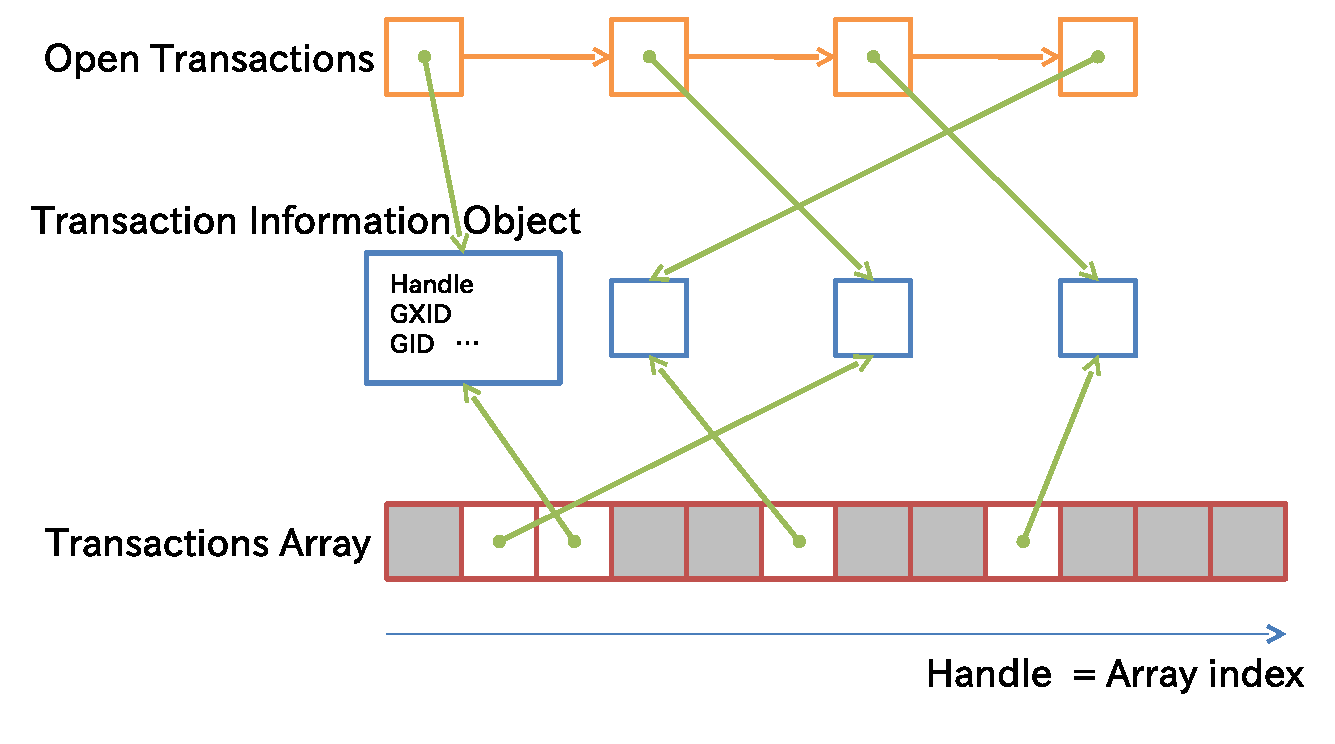
\includegraphics[width=0.8\hsize]{add_gtmtxn.eps}
		  \caption{\label{fig:addgtmtxn}Transaction management in GTM}
	  \end{center}
  \end{figure}
  
  Note: Some codes seems to be copied from \file{transam.c}.
  
  
  \FUNC{GTM\_HandleToTransactionInfo()}	%--------------------------------------
  
    Finds the corresponding transaction info structure by the transaction handle.
    %
    This is called from the following codes:
    
    \FuncRefHdr
		\FuncRef{-}{gtm_txn.c}{
		  \vspace{3pt}
		}\\
		\FuncRef{GTM_GetTransactionSnapshot}{gtm_snap.c}{
		  Used in taking the transaction snapshot to check and store information with given handles.
		}\\ \hline
    \FuncRefTrailor
  
  \FUNC{GTM_GXIDToHandle()}	%--------------------------------------
  
	Finds the transaction handle corresponding to given GXID.
    %
    This is called from the following codes:
    
    \FuncRefHdr
		\FuncRef{-}{gtm_txn.c}{
		  \vspace{3pt}
		}\\
		\FuncRef{ProcessGetSnapshotCommand}{gtm_snap.c}{
			Used in processing \file{MSG_SNAPSHOT_GET} command to obtain the handle from given
			GXID for querying the transaction information.
		}\\
		\FuncRef{ProcessGetSnapshotCommandMulti}{gtm_snap.c}{
			Used in processing \file{MSG_SNAPSHOT_GET_MULTI} command to obtain the handle from
			given GXID for querying the transaction information.
		}\\ \hline
    \FuncRefTrailor
  
  \FUNC{GTM_GIDToHandle()}	%--------------------------------------
  
	Finds the transaction handle corresponding to the 
    given the GID (for a prepared transaction).
    %
    This function is used by only the functions in the same file.
  
  \FUNC{GTM_InitTxnManager()}	%--------------------------------------
  
    Initializes global variables of the transaction manager.
    %
    This is called from the following codes:
    
    \FuncRefHdr
		\FuncRef{BaseInit}{main.c}{
		  Used in start up sequence.
		}\\ \hline
    \FuncRefTrailor
  
  \FUNC{GTM_BeginTransaction()}	%--------------------------------------
  
    Begins a new transaction and return assigned handle.
    
    This function creates new transaction object and register it into opend transaction list.
    
    This is called from the following codes:
    
	{
		\footnotesize
		\FuncRefHdr
			\FuncRef{ProcessBeginTransactionCommand}{gtm_txn.c}{
			  Used in processing \file{MSG_TXN_BEGIN} message
			}\\
			\FuncRef{ProcessBeginTransactionGetGXIDCommand}{gtm_txn.c}{
			  Used in processing \file{MSG_TXN_BEGIN_GETGXID} message
			}\\
			\FuncRef{ProcessBeginTransactionGetGXIDAutovacuumCommand}{gtm_txn.c}{
			  Used in processing \file{MSG_TXN_BEGIN_GETGXID_AUTOVACUUM} message
			}\\
			\FuncRef{ProcessGetGIDDataTransactionCommand}{gtm_txn.c}{
			  Used in processing \file{MSG_TXN_GET_GID_DATA} message
			}\\ \hline
		\FuncRefTrailor
	}
  
  
  \FUNC{GTM_BeginTransactionMulti()}	%--------------------------------------
  
    Begins a new transactions and returns number of new transactions began.
    
    This function delegates internal logic to \file{GTM_BeginTransaction}.
    
    This is called from the following codes:
    
	{
		\footnotesize
		\FuncRefHdr
			\FuncRef{GTM_BeginTransaction}{gtm_txn.c}{
			  Delegates internal logic
			}\\
			\FuncRef{ProcessBeginTransactionGetGXIDCommandMulti}{gtm_txn.c}{
			  Used in processing \file{MSG_TXN_BEGIN_GETGXID_MULTI} message
			}\\ \hline
		\FuncRefTrailor
	}
  
  \FUNC{GTM_RollbackTransaction()}	%--------------------------------------
  
	  Rolls back a transaction by handle.
	  
	  This function delegates internal logic to \file{GTM_RollbackTransactionMulti}.
	  
	  This is called from the following codes:
	  
	  {
		  \footnotesize
		  \FuncRefHdr
			  \FuncRef{GTM_RollbackTransactionGXID}{gtm_txn.c}{
				Convert GXID to handle and delegates internal logic
			  }\\
			  \FuncRef{ProcessRollbackTransactionCommand}{gtm_txn.c}{
				Used in processing \file{MSG_TXN_ROLLBACK} / \file{MSG_BKUP_TXN_ROLLBACK} message
			  }\\ \hline
		  \FuncRefTrailor
	  }
  
  \FUNC{GTM_RollbackTransactionMulti()}	%--------------------------------------
  
    Rolls back transactions by handles.
    
    This function marks transactions as ``rollback in progress'' and removes them from opend transaction list.
    
    This is called from the following codes:
    
    \FuncRefHdr
		\FuncRef{GTM_RollbackTransaction}{gtm_txn.c}{
		  Delegates internal logic
		}\\
		\FuncRef{ProcessRollbackTransactionCommandMulti}{gtm_txn.c}{
		  Used in processing \file{MSG_TXN_ROLLBACK_MULTI} or \file{MSG_BKUP_TXN_ROLLBACK_MULTI} message
		}\\
		\hline
    \FuncRefTrailor
  
  \FUNC{GTM_RollbackTransactionGXID()}	%--------------------------------------
  
    Rolls back transaction by GXID
    
    This function converts GXID to the handle and delegates internal logic to  \file{GTM_RollbackTransaction}.
    
    This function is never used.
  
  \FUNC{GTM_CommitTransaction()}	%--------------------------------------
  
    Commits a transaction by handle.
    
    This function delegates internal logic to \file{GTM_CommitTransactionMulti}.
    
    This is called from the following codes:
    
    \FuncRefHdr
		\FuncRef{GTM_CommitTransactionGXID}{gtm_txn.c}{
		  Convert GXID to handle and delegates internal logic
		}\\
		\FuncRef{ProcessCommitTransactionCommand}{gtm_txn.c}{
		  Used in processing \file{MSG_TXN_COMMIT} message
		}\\ \hline
    \FuncRefTrailor
  
  \FUNC{GTM_CommitTransactionMulti()}	%--------------------------------------
  
    Commits transactions by handles.
    
    This function marks transactions as ``commit in progress'' and removes them from opend transaction list.
    
    This is called from the following codes:

	{
		\footnotesize
		\FuncRefHdr
			\FuncRef{GTM_CommitTransaction}{gtm_txn.c}{
			  Delegates internal logic
			}\\
			\FuncRef{ProcessCommitPreparedTransactionCommand}{gtm_txn.c}{
			  Used in processing \file{MSG_TXN_COMMIT_PREPARED} / \file{MSG_BKUP_TXN_COMMIT_PREPARED} message
			}\\
			\FuncRef{ProcessCommitTransactionCommandMulti}{gtm_txn.c}{
			  Used in processing \file{MSG_TXN_COMMIT_MULTI} / \file{MSG_BKUP_TXN_COMMIT_MULTI} message
			}\\ \hline
		\FuncRefTrailor
	}
  
  \FUNC{GTM_CommitTransactionGXID()}	%--------------------------------------
  
    Commits a transaction by GXID.
    
    This function converts GXID to the handle and delegates internal logic to  \file{GTM_CommitTransaction}.
    
    This function is not used at present.
  
  \FUNC{GTM_PrepareTransaction()}	%--------------------------------------
  
    Prepares a transaction by the handle.
    
    This function marks transaction as ``prepared''.
    
    This is called from the following codes:
    
	{
		\footnotesize
		\FuncRefHdr
			\FuncRef{ProcessPrepareTransactionCommand}{gtm_txn.c}{
			  Used in processing \file{MSG_TXN_PREPARE} / \file{MSG_BKUP_TXN_PREPARE} message
			}\\ \hline
		\FuncRefTrailor
	}
  
  \FUNC{GTM_StartPreparedTransaction()}	%--------------------------------------
  
    Starts to prepare a transaction by the handle.
    
    This function save GID and marks transactions as ``prepare in progress''.
    
    This is called from the following codes:
    
	{
		\footnotesize
		\FuncRefHdr
			\FuncRef{GTM_StartPreparedTransactionGXID}{gtm_txn.c}{
			  Converts GXID to the handle and delegates internal logic
			}\\
			\FuncRef{ProcessStartPreparedTransactionCommand}{gtm_txn.c}{
			  Used in processing \file{MSG_TXN_START_PREPARED} / \file{MSG_BKUP_TXN_START_PREPARED} message
			}\\ \hline
		\FuncRefTrailor
	}
  
  \FUNC{GTM_StartPreparedTransactionGXID()}	%--------------------------------------
  
    Starts to prepare a transaction by GXID.
    
    This function converts GXID to the handle and delegates internal logic to  \file{GTM_StartPreparedTransaction}.
    
    This function is not used at present.
  
  \FUNC{GTM_GetGIDData()}	%--------------------------------------
  
    Gets information of a prepared transaction.
    %
    This is called from the following codes:
    
	{
		\footnotesize
		\FuncRefHdr
			\FuncRef{ProcessGetGIDDataTransactionCommand}{gtm_txn.c}{
			  Used in processing \file{MSG_TXN_GET_GID_DATA} message
			}\\ \hline
		\FuncRefTrailor
	}
  
  \FUNC{GTM_GetAllPrepared()}	%--------------------------------------
  
    \textbf{Not implemented yet}
  
  \FUNC{GTM_GetStatus()}	%--------------------------------------
  
    Gets transaction status.
    %
    This is called from the following codes:
    
    \FuncRefHdr
		\FuncRef{GTM_GetStatusGXID}{gtm_txn.c}{
		  Convert GXID to handle and delegates internal logic
		}\\
		\hline
    \FuncRefTrailor
  
  \FUNC{GTM_GetStatusGXID()}	%--------------------------------------
  
    Gets transaction status by GXID.
    
    This function converts GXID to handle and delegates internal logic to  \file{GTM_GetStatus}.
    
    This function is never used.
  
  \FUNC{GTM_GetAllTransactions()}	%--------------------------------------
  
    \textbf{Not implemented yet}
  
  \FUNC{GTM_RemoveAllTransInfos()}	%--------------------------------------
  
    Removes all the transaction information associated with the caller thread and the given backend.
    
    This function removes all the transaction information associated with the caller thread and the given backend from opened transaction list.
    This also calculates \texttt{latestCompletedXid}.
    
    This function is used to clear implicitly aborted transactions when a backend or a GTM proxy disconnect without committing, aborting and preparing.
    
    This is called from the following codes:
    
    \FuncRefHdr
		\FuncRef{GTM_ThreadMain}{main.c}{
		  Called when the message loop detected a backend disconnection.
		}\\
		\FuncRef{ProcessCommand}{main.c}{
		  Used in processing \file{MSG_BACKEND_DISCONNECT}
		}\\
		\hline
    \FuncRefTrailor


% - - - - subsubsection - - - - - - -  - - - - - - - - - - - - - - - - - - - - -

\subsubsection{gtm\_snap.c}

  This module supplies snapshot handling functions on GTM.
  
  \FUNC{GTM_GetSnapshotData()}	%--------------------------------------
  
    \textbf{Not implemented yet}
  
  \FUNC{GTM_GetTransactionSnapshot()}	%--------------------------------------
  
    Gets snapshot for the given transactions.
    
    This function takes transaction snapshots and saves to transaction information object.
    
    Although this function looks supporting \texttt{SERIALIZABLE} isolation level, the code is not complete.
    It doesn't a matter as long as \texttt{READ COMMITTED} isolation level is used.
    
    This is called from the following codes:
    
    \FuncRefHdr
		\FuncRef{ProcessGetSnapshotCommand}{gtm_snap.c}{
		  Used in processing \file{MSG_SNAPSHOT_GET}
		}\\
		\FuncRef{ProcessGetSnapshotCommandMulti}{gtm_snap.c}{
		  Used in processing \file{MSG_SNAPSHOT_GET_MULTI}
		}\\ \hline
    \FuncRefTrailor
  
  \FUNC{GTM_FreeCachedTransInfo()}	%--------------------------------------
  
    \textbf{Not implemented yet}
  
  \FUNC{GTM_BkupBeginTransactionMulti()}	%--------------------------------------
  
    Updates global transaction information to given ones.
    %
    This is called from the following codes:
    
    \FuncRefHdr
		\FuncRef{GTM_BkupBeginTransaction}{gtm_txn.c}{
		  Delegate internal logic
		}\\ \hline
    \FuncRefTrailor
  
  \FUNC{ProcessBeginTransactionCommandMulti()}	%--------------------------------------
  
    \textbf{Not implemented yet}
  
  
  \FUNC{GTM_SaveTxnInfo()}	%--------------------------------------
  
    Saves next GXID to the control file.
    %
    This is called from the following codes:
    
    \FuncRefHdr
		\FuncRef{GTM_MakeBackup}{gtm_backup.c}{
		  Used to save next GXID to the backup file
		}\\
		\FuncRef{ServerLoop}{main.c}{
		  Used in shutdown sequence
		}\\ \hline
    \FuncRefTrailor
  
  \FUNC{GTM_RestoreTxnInfo()}	%--------------------------------------
  
    Restores the next GXID from the control file.
    
    This function also sets \file{latestCompletedXid}.
    If the control file is not available, it uses given value
	from a \texttt{gtm} command line option.
    
    This is called from the following codes:
    
    \FuncRefHdr
		\FuncRef{gtm_standby_restore_next_gxid}{gtm_standby.c}{
		  \file{GTM_RestoreTxnInfo(NULL, next_gxid);}
		}\\
		\FuncRef{main}{main.c}{
		  Used in start up sequence
		}\\ \hline
    \FuncRefTrailor
  
  \FUNC{GTM_BkupBeginTransaction()}	%--------------------------------------
  
    Updates global transaction information to given one.
    
    This function delegates internal logic to  \file{GTM_BeginTransaction}.
    
    This is called from the following codes:
    
	{
		\footnotesize
		\FuncRefHdr
			\FuncRef{ProcessBkupBeginTransactionCommand}{gtm_txn.c}{
			  Used in processing \file{MSG_BKUP_TXN_BEGIN} message
			}\\ \hline
		\FuncRefTrailor
	}
  
  
  \FUNC{GTM_FreeSnapshotData()}	%--------------------------------------
  
    Releases the snapshot data
    
    This function releases the snapshot data.
    Please note that the snapshot itself is not freed by this function.
    
    This function is not used at present.



% - - - - subsubsection - - - - - - -  - - - - - - - - - - - - - - - - - - - - -

\subsubsection{\texttt{gtm\_seq.c}}

  This module supplies Sequence handling infrastructure.
  This is one of the most importarnt part of GTM.
  
  An instance of {\file{struct} \file{GTM_SeqInfo}} is created corresponding to a sequence in a database.
  The structure is shown in Table \ref{tab:gtmseqinfo}.
  Most of the member variables has corresponding \PG's sequence attribute.
  \file{gs_ref_count} is a GTM specific variable which manages reference to automatic
  destruction of the sequence, but there's no case that the sequence is destroyed by
  the reference count.
  
  The sequence information is stored into \file{GTMSequences} global hash table.
  Sequence information is distributed by the hash value of their name 
  so that character string comparison is not needed afterwords.
  
  \begin{table}[htp]
	  \begin{center}
		  \caption{\label{tab:gtmseqinfo}{Members of \texttt{struct GTM\_SeqInfo}}}\vspace{5pt}
		  \begin{tabular}{lp{0.6\hsize}} \hline
			Member variable & Description \\ \hline
			\file{gs_key} & Same as \file{sequence_name} of the sequence in \PG. \\
			\file{gs_value} & Same as \file{last_value} of the sequence in \PG. \\
			\file{gs_backedUpValue}
				& The last value of the sequence which is backuped to the control file. \\
			\file{gs_init_value} & Same as \file{start_value} of the sequence in \PG. \\
			\file{gs_last_value} & \textit{Updated but not used at present}. \\
			\file{gs_increment_by} & Same as \file{increment_bu} of the sequence in \PG. \\
			\file{gs_min_value} & Same as \file{min_value} of the sequence in \PG. \\
			\file{gs_max_value} & Same as \file{max_value} of the sequence in \PG. \\
			\file{gs_cycle} & Same as \file{is_cycled} of the sequence in \PG. \\
			\file{gs_called} & Same as \file{is_called} of the sequence in \PG. \\
			\file{gs_ref_count} & The reference count of the sequence object. \\
			\file{gs_state} & The state of the sequence. This variable could take
							  \file{SEQ_STATE_ACTIVE | SEQ_STATE_DELETED}.\\
			\file{gs_lock} & The lock for the sequence object.\\
			\hline
		  \end{tabular}
	  \end{center}
  \end{table}
  
  
  \FUNC{GTM_InitSeqManager()}	%--------------------------------------
  
    Initializes global variable for the sequence manager.
    %
    This is called from the following codes:
    
    \FuncRefHdr
		\FuncRef{BaseInit}{main.c}{
		  Used in start up sequence
		}\\ \hline
    \FuncRefTrailor
  
  \FUNC{GTM_SeqOpen()}	%--------------------------------------
  
    Initializes a new sequence.
    
    This function initializes a new sequence.
    Optionally set the initial value of the sequence.
    
    This is called from the following codes:
    
    \FuncRefHdr
		\FuncRef{ProcessSequenceInitCommand}{gtm_seq.c}{
		  Used in processing \file{MSG_SEQUENCE_INIT} message
		}\\ \hline
    \FuncRefTrailor
  
  \FUNC{GTM_SeqAlter()}	%--------------------------------------
  
    Alter a sequence.
    
    This function alternates current sequence parameters and given one.
    This function can't rename the sequence.
    
    This is called from the following codes:
    
    \FuncRefHdr
		\FuncRef{ProcessSequenceAlterCommand}{gtm_seq.c}{
		  Used in processing Process \file{MSG_SEQUENCE_ALTER} / \file{MSG_BKUP_SEQUENCE_ALTER} / \file{MSG_BKUP_SEQUENCE_ALTER} message
		}\\ \hline
    \FuncRefTrailor
  
  \FUNC{GTM_SeqClose()}	%--------------------------------------
  
    Destroys the given sequence depending on the type of given key
    
    This function can take a sequence name or a database name.
    If a sequence name is given, it destroys the sequence.
    If database name is given, it destroys all of the sequences belogs to the database using prefix of full quolified sequence name.
    Latter functionarity is used when dropping a database.
    
    This is called from the following codes:
    
    \FuncRefHdr
		\FuncRef{GTM_SeqRename}{gtm_seq.c}{
		  Used in renaming sequence to destroy old sequence info.
		}\\
		\FuncRef{ProcessSequenceCloseCommand}{gtm_seq.c}{
		  Used in processing \file{MSG_SEQUENCE_CLOSE} / \file{MSG_BKUP_SEQUENCE_CLOSE} / \file{MSG_BKUP_SEQUENCE_CLOSE} message
		}\\ \hline
    \FuncRefTrailor
  
  \FUNC{GTM_SeqRename()}	%--------------------------------------
  
    Rename an existing sequence with a new name
    
    This function creates a new sequence object and copies parameters from old one,
	which is destroyed then.
    
    This is called from the following codes:
    
    \FuncRefHdr
		\FuncRef{ProcessSequenceRenameCommand}{gtm_seq.c}{
		  Used in processing \file{MSG_SEQUENCE_RENAME} / \file{MSG_BKUP_SEQUENCE_RENAME} / \file{MSG_BKUP_SEQUENCE_RENAME} message
		}\\ \hline
    \FuncRefTrailor
  
  \FUNC{GTM_SeqGetNext()}	%--------------------------------------
  
    Gets the next value for the sequence.
    %
    This is called from the following codes:
    
    \FuncRefHdr
		\FuncRef{ProcessSequenceGetNextCommand}{gtm_seq.c}{
		  Used in processing \file{MSG_SEQUENCE_GET_NEXT} / \file{MSG_BKUP_SEQUENCE_GET_NEXT} / \file{MSG_BKUP_SEQUENCE_GET_NEXT} message.
		}\\ \hline
    \FuncRefTrailor
  
  \FUNC{GTM_SeqSetVal()}	%--------------------------------------
  
    Sets values for the sequence.
    %
    This is called from the following codes:
    
    \FuncRefHdr
		\FuncRef{ProcessSequenceSetValCommand}{gtm_seq.c}{
		  Used in processing \file{MSG_SEQUENCE_SET_VAL} / \file{MSG_BKUP_SEQUENCE_SET_VAL} /
		  \file{MSG_BKUP_SEQUENCE_SET_VAL} message.
		}\\ \hline
    \FuncRefTrailor
  
  \FUNC{GTM_SeqReset()}	%--------------------------------------
  
    Resets the sequence.
    %
    This is called from the following codes:
    
    \FuncRefHdr
		\FuncRef{ProcessSequenceResetCommand}{gtm_seq.c}{
		  Used in processing \file{MSG_SEQUENCE_RESET} / \file{MSG_BKUP_SEQUENCE_RESET} /
		  \file{MSG_BKUP_SEQUENCE_RESULT} message.
		}\\ \hline
    \FuncRefTrailor
  
  \FUNC{GTM_SaveSeqInfo()}	%--------------------------------------
  
    Saves all the sequence information.
    
    This is called from the following codes:
    
    \FuncRefHdr
		\FuncRef{GTM_MakeBackup}{gtm_backup.c}{
		  Used in making a backup file.
		  This function is never used.
		}\\
		\FuncRef{ServerLoop}{main.c}{
		  Used in shutting down sequence to save sequence information for next run.
		}\\ \hline
    \FuncRefTrailor
  
  \FUNC{GTM_RestoreSeqInfo()}	%--------------------------------------
  
    Restores sequence information from the control file.
    
	\begin{itemize}
		\item This function is used only by the functions in the same file.
		\item This is also called from the following codes:
	\end{itemize}
    
    \FuncRefHdr
		\FuncRef{main}{main.c}{
		  \file{GTM_RestoreSeqInfo(ctlf);}`
		}\\
		\hline
    \FuncRefTrailor
  
  \FUNC{GTM_SeqRestore()}	%--------------------------------------
  
    Restores a sequence.
    %
    This is called from the following codes:
    
    \FuncRefHdr
		\FuncRef{GTM_RestoreSeqInfo}{gtm_seq.c}{
		  Used in restoring sequences information from a file, which is typically the control file
		}\\
		\FuncRef{gtm_standby_restore_sequence}{gtm_standby.c}{
		  Used in restoring sequences information from a GTM master
		}\\ \hline
    \FuncRefTrailor
  
  \FUNC{GTM_NeedSeqRestoreUpdate()}	%--------------------------------------
  
    Tests if backup data needs update after the given sequence is touched.
    
    This function is not used at present.
  
  \FUNC{GTM_WriteRestorePointSeq()}	%--------------------------------------
  
    Writes the restoration point of all the sequences.
    
    This function saves restore point of all sequences to the file, which is typically the control file.
    The restore point is saved to deal with abnormal termination of GTM, they are advanced 2000 count to
	current value at maximum to avoid frequent disk write.
    
    This is called from the following codes:
    
    \FuncRefHdr
		\FuncRef{GTM_WriteRestorePoint}{gtm_backup.c}{
		  Used in making the control file to write sequences information
		}\\
		\FuncRef{GTM_WriteBarrierBackup}{gtm_backup.c}{
		  Used in making a barrier file to write sequences information
		}\\ \hline
    \FuncRefTrailor



% - - - - subsubsection - - - - - - -  - - - - - - - - - - - - - - - - - - - - -

\subsubsection{\texttt{gtm\_thread.c}}

  This module supplies thread handling functions.
  
  The things to note here is thread-specific data is stored in \file{GTM_ThreadInfo}
  structure.
  It is allocated in thread-local storage and we can access it using \file{GetMyThreadInfo} macro.
  \file{GetMyThreadInfo} uses pthread function to obtain the pointer and the key
  \file{threadinfo_key} is created in \file{main.c} and \file{main_proxy.c}.
  
  \file{MyPort} macro is implicitly used in libpq functions to determine what connection to use.
  This macro is redefined in GTM to refer to variables in thread-specific data.
  This change reduces much effort to port libpq into thread model.
  
  Memory contexts are similar to the case of \file{MyPort}.
  Many memory contexts such as \file{TopMemoryContext}, \file{ErrorContext}, \file{MessageContext} and
  \file{CurrentMemoryContext}, are stored in \file{GTM_ThreadInfo} for each thread and
  corresponding macros are also redefined.
  All of the memory allocated with these context are freed by thread cleanup function when the thread exits.
  
  \FUNC{GTM_ThreadAdd()}	%--------------------------------------
  
    Adds the given thrinfo structure to the global array.
    
    This function adds the given thrinfo structure to the global array.
    If the array is full, it expands it automatically.
    
    This is called from the following codes:
    
    \FuncRefHdr
		\FuncRef{GTM_ThreadCreate}{gtm_thread.c}{
		  Used in creating a new thread for a GTM client.
		}\\
		\FuncRef{BaseInit}{main.c}{
		  Used in the initialization of the main thread.
		}\\ \hline
    \FuncRefTrailor
  
  \FUNC{GTM_ThreadRemove()}	%--------------------------------------
  
    Removes given \file{GTM_ThreadInfo} structure from the global array.
    
    This is called from the following codes:
    
    \FuncRefHdr
		\FuncRef{GTM_ThreadCleanup}{gtm_thread.c}{
		  Used in cleaning up of a thread
		}\\ \hline
    \FuncRefTrailor
  
  \FUNC{GTM_ThreadJoin()}	%--------------------------------------
  
    Waits for exitting of given thread.
    
    This function is not used at present.
  
  \FUNC{GTM_ThreadExit()}	%--------------------------------------
  
    Exits this thread immediately.
    
    This function is not used at present.
  
  \FUNC{GTM_LockAllOtherThreads()}	%--------------------------------------
  
    Locks all the thread information objects of all other threads.
    
    This function is not used at present.
  
  \FUNC{GTM_UnlockAllOtherThreads()}	%--------------------------------------
  
    Unlocks all the information objects of all the other threads.
    
    This function is not used at present.
  
  \FUNC{GTM_DoForAllOtherThreads()}	%--------------------------------------
  
    Invokes callback function function for each of other thread information objects.
    %
    This is called from the following codes:
    
    \FuncRefHdr
		\FuncRef{ProcessPGXCNodeRegister}{register_gtm.c}{
		  Used in processing \file{MSG_NODE_REGISTER} message to disconnect connections to GTM slave in all threads when new GTM standby is registered.
		}\\ \hline
    \FuncRefTrailor
  
  \FUNC{GTM_ThreadCreate()}	%--------------------------------------
  
    Creates a new thread and assigns the given connection to it.
    
    This function creates a new thread, thread local memory contexts and a thread information object, and assign the given connection to the thread.
    
    This is called from the following codes:
    
    \FuncRefHdr
		\FuncRef{GTMAddConnection}{main.c}{
		  Used in adding new connection from a GTM client.
		}\\ \hline
    \FuncRefTrailor
  
  \FUNC{GTM_GetThreadInfo()}	%--------------------------------------
  
    \textit{Not implemented yet.}
  
  

% - - - - subsubsection - - - - - - -  - - - - - - - - - - - - - - - - - - - - -

\subsubsection{\texttt{gtm\_backup.c}}
  
  This module supplies backup functions on GTM.
  
  \FUNC{GTM_WriteRestorePoint()}	%--------------------------------------
  
    Writes restoration point.
    
    This function saves restoration point of GXID and sequences to the control file.
    The restore point is saved to deal with abnormal termination of GTM.
   	They are advanced 2000 count to current value at maximum.
    
    This is called from the following codes:
    
    \FuncRefHdr
		\FuncRef{main}{main.c}{
		  Used in start up sequence after all the data are restored.
		}\\
		\FuncRef{ProcessCommand}{main.c}{
		  Used in main loop when backup is needed.
		}\\
		\FuncRef{PromoteToActive}{main.c}{
		  Used in promoting to activate.
		}\\ \hline
    \FuncRefTrailor
  
  \FUNC{GTM_MakeBackup()}	%--------------------------------------
  
    Saves the next GXID and sequence information to given backup file.
    
    This function is not used at present.
  
  \FUNC{GTM_SetNeedBackup()}	%--------------------------------------
  
    Set \textbf{need backup} flag to true
    
    This function sets \textbf{need backup} flag to true.
    This flag means transaction or sequence information are need to be saved.
    
    This is called from the following codes:
    
    \begin{itemize}
      \item When the sequence value is created or jumped or removed.
      \item When the sequence value is incremented and it catches up with backed-up value.
      \item When GXID is incremented and it catches up with backed-up value.
    \end{itemize}
  
  \FUNC{GTM_NeedBackup()}	%--------------------------------------
  
    Tests \textbf{need backup} flag.
    %
    This is called from the following codes:
    
    \FuncRefHdr
		\FuncRef{ProcessCommand}{main.c}{
		  Used in message loop to decide whether do backup or not.
		}\\ \hline
    \FuncRefTrailor
  
  \FUNC{GTM_WriteBarrierBackup()}	%--------------------------------------
  
    Creates GTM restration point file corresponding to a barrier.
    %
    This is called from the following codes:
    
    \FuncRefHdr
		\FuncRef{ProcessBarrierCommand}{main.c}{
		  Used in processing \file{MSG_BARRIER} / \file{MSG_BKUP_BARRIER} message
		}\\ \hline
    \FuncRefTrailor



% - - - - subsubsection - - - - - - -  - - - - - - - - - - - - - - - - - - - - -

\subsubsection{\texttt{gtm\_standby.c}}

  This module supplies functionalities of GTM Standby.
  
  \FUNC{gtm_is_standby()}	%--------------------------------------
  
    \textbf{Not implemented yet.}
  
  \FUNC{gtm_set_standby()}	%--------------------------------------
  
    \textbf{Not implemented yet.}
  
  \FUNC{gtm_set_active_conninfo()}	%--------------------------------------
  
    \textbf{Not implemented yet.}
  
  \FUNC{gtm_standby_start_startup()}	%--------------------------------------
  
    Initializes GTM standby startup.
    
    This function connects to GTM active and initialize locks for standby mode.
    
    This is called from the following codes:
    
    \FuncRefHdr
		\FuncRef{main}{main.c}{
		  Used in start up sequence of GTM standby
		}\\ \hline
    \FuncRefTrailor
  
  \FUNC{gtm_standby_finish_startup()}	%--------------------------------------
  
    Finishes GTM standby startup
    
    This function closes connection to GTM active for connect-back from master.
    
    This is called from the following codes:
    
    \FuncRefHdr
		\FuncRef{main}{main.c}{
		  Used in start up sequence of GTM standby
		}\\ \hline
    \FuncRefTrailor
  
  \FUNC{gtm_standby_restore_next_gxid()}	%--------------------------------------
  
    Gets the next GXID value from GTM active.
    %
    This is called from the following codes:
    
    \FuncRefHdr
		\FuncRef{main}{main.c}{
		  Used in start up sequence of GTM standby
		}\\ \hline
    \FuncRefTrailor
  
  \FUNC{gtm_standby_restore_gxid()}	%--------------------------------------
  
    Restores global transaction information from GTM active.
    %
    This is called from the following codes:
    
    \FuncRefHdr
		\FuncRef{main}{main.c}{
		  Used in start up sequence of GTM standby
		}\\ \hline
    \FuncRefTrailor
  
  \FUNC{gtm_standby_restore_sequence()}	%--------------------------------------
  
    Restores sequence information from GTM active.
    %
    This is called from the following codes:
    
    \FuncRefHdr
		\FuncRef{main}{main.c}{
		  Used in start up sequence of GTM standby
		}\\ \hline
    \FuncRefTrailor
  
  \FUNC{gtm_standby_restore_node()}	%--------------------------------------
  
    Restores node information from GTM active.
    %
    This is called from the following codes:
    
    \FuncRefHdr
		\FuncRef{main}{main.c}{
		  Used in start up sequence of GTM standby
		}\\ \hline
    \FuncRefTrailor
  
  \FUNC{gtm_standby_register_self()}	%--------------------------------------
  
    Registers itself to the GTM active as a ``disconnected'' node.
    
    This function registers myself to the GTM active as a ``disconnected'' node before restore starts.
    This status would be updated later after restoring completion.
    
    This function's comment saids above, but \file{PorcessPGXCNodeRegister()} which processes \file{MSG_NODE_REGISTER} message ignores the status ``disconnected''.
    
    This is called from the following codes:
    
    \FuncRefHdr
		\FuncRef{main}{main.c}{
		  Used in start up sequence of GTM standby
		}\\ \hline
    \FuncRefTrailor
  
  \FUNC{gtm_standby_activate_self()}	%--------------------------------------
  
    Update node status of itself from "disconnected" to "connected" in GTM active.
    
    This function unregisters myself once, after that it registers myself again as ``connected'' node.
    
    This is called from the following codes:
    
    \FuncRefHdr
		\FuncRef{main}{main.c}{
		  Used in start up sequence of GTM standby
		}\\ \hline
    \FuncRefTrailor
  
  \FUNC{gtm_standby_connect_to_standby()}	%--------------------------------------
  
    Makes a connection to the GTM standby.
    
    This is called from the following codes:
    
    \FuncRefHdr
		\FuncRef{ServerLoop}{main.c}{
		  Used in GTM active accept loop when a GTM client connected.
		}\\
		\FuncRef{GTM_ThreadMain}{main.c}{
		  Used in GTM active message loop when a GTM slave newly registered.
		}\\ \hline
    \FuncRefTrailor
  
  \FUNC{gtm_standby_disconnect_from_standby()}	%--------------------------------------
  
    Disconnects connection from GTM standby.
    
    This function disconnects given connection if it is not in standby mode.
    
    This is called from the following codes:
    
    \FuncRefHdr
		\FuncRef{gtm_standby_reconnect_to_standby}{gtm_standby.c}{
		  Used in reconnection to GTM standby to close old connection.
		}\\
		\FuncRef{ServerLoop}{main.c}{
		  Used in accept loop to cancel connection to GTM standby when GTM can't accept more connection.
		}\\
		\FuncRef{GTM_ThreadMain}{main.c}{
		  Used in message loop to close existing connection to GTM standby when GTM standby is unregistered.
		}\\ \hline
    \FuncRefTrailor
  
  \FUNC{gtm_standby_reconnect_to_standby()}	%--------------------------------------
  
    Reconnects to GTM standby.
    
    This function closes old connection and reconnects to GTM standby if it is not in standby mode.
    
    This is called from the following codes:
    
    \FuncRefHdr
		\FuncRef{gtm_standby_check_communication_error}{gtm_standby.c}{
		  Used in checking communication error with standby when it detects an error.
		}\\ \hline
    \FuncRefTrailor
  
  \FUNC{gtm_standby_check_communication_error()}	%--------------------------------------
  
    Checks if communication with standby made an error.
    
    This function checks whether the communication with standby made an error.
	If an error is detected, it reconnects to GTM standby.
    
    This is called from everywhere which makes interaction with GTM standby.
  
  \FUNC{find_standby_node_info()}	%--------------------------------------
  
    Finds ``one'' GTM standby node info.
    
    This function returns node information of GTM standby.
    Please note that GTM cannot have multiple GTM standby nodes.
    
    This is called from the following codes:
    
    \FuncRefHdr
		\FuncRef{gtm_standby_connect_to_standby_int}{gtm_standby.c}{
		  Used in connecting to GTM standby
		}\\
		\FuncRef{ProcessPGXCNodeRegister}{register_gtm.c}{
		  Used in processing \file{MSG_NODE_REGISTER} message to check the standby node has not been registered yet.
		}\\ \hline
    \FuncRefTrailor
  
  \FUNC{gtm_standby_begin_backup()}	%--------------------------------------
  
    Notifies GTM standby is beginning backup of GTM active.
    %
    This is called from the following codes:
    
    \FuncRefHdr
		\FuncRef{main}{main.c}{
		  Used in start up sequence of GTM standby
		}\\ \hline
    \FuncRefTrailor
  
  \FUNC{gtm_standby_end_backup()}	%--------------------------------------
  
    Notifies GTM standby is ending backup of GTM active.
    %
    This is called from the following codes:
    
    \FuncRefHdr
		\FuncRef{main}{main.c}{
		  Used in start up sequence of GTM standby
		}\\ \hline
    \FuncRefTrailor
  
  \FUNC{gtm_standby_closeActiveConn()}	%--------------------------------------
  
    \textit{Not implemented yet.}
  
  \FUNC{gtm_standby_finishActiveConn()}	%--------------------------------------
  
    Unregisters itself from GTM active.
    
    This function is not used at present.
  
  \FUNC{ProcessGTMBeginBackup()}	%--------------------------------------
  
    Handler of \file{MSG_BEGIN_BACKUP}.
    
    This function sets thread status to \file{GTM_THREAD_BACKUP} and locks all of other thread information objects.
    This function also sends a result immediately to GTM standby.
    
    This is called from the following codes:
    
    \FuncRefHdr
		\FuncRef{ProcessCommand}{main.c}{
		  Used in processing \file{MSG_BEGIN_BACKUP}
		}\\ \hline
    \FuncRefTrailor
  
  \FUNC{ProcessGTMEndBackup()}	%--------------------------------------
  
    Processes \file{MSG_END_BACKUP}.
    
    This function resets thread status to \file{GTM_THREAD_RUNNING} from \file{GTM_THREAD_BACKUP} and unlocks all of other thread information objects.
    This function also sends a result immediately to GTM standby.
    
    This is called from the following codes:
    
    \FuncRefHdr
		\FuncRef{ProcessCommand}{main.c}{
		  Used in processing \file{MSG_END_BACKUP}
		}\\ \hline
    \FuncRefTrailor


% - - - - subsubsection - - - - - - -  - - - - - - - - - - - - - - - - - - - - -

\subsubsection{\texttt{gtm\_time.c}}

  This module supplies timestamp handling functions on GTM.
  
  \FUNC{GTM_TimestampGetCurrent()}	%--------------------------------------
  
    Gets the current timestamp.
    %
    This is called from the following codes:
    
	{
		\footnotesize
		\FuncRefHdr
			\FuncRef{ProcessBeginTransactionCommand}{gtm_txn.c}{
			  Used to get transaction start timew
			}\\
			\FuncRef{ProcessBeginTransactionGetGXIDCommand}{gtm_txn.c}{
			  Used to get transaction start timew
			}\\
			\FuncRef{ProcessBeginTransactionGetGXIDCommandMulti}{gtm_txn.c}{
			  Used to get transaction start timew
			}\\ \hline
		\FuncRefTrailor
	}



% - - - - subsubsection - - - - - - -  - - - - - - - - - - - - - - - - - - - - -

\subsubsection{\texttt{replication.c}}

  This module supplies controlling the initialization and end of replication process of GTM data.
  These function is implemented but never used in \XC, so explanations are omitted.



% - - - - subsubsection - - - - - - -  - - - - - - - - - - - - - - - - - - - - -

\subsubsection{\texttt{gtm\_stat.c}}

  This module is not implemented yet.



% - - - - subsubsection - - - - - - -  - - - - - - - - - - - - - - - - - - - - -

\subsubsection{\texttt{gtm\_stats.c}}

  This module is not implemented yet.



%------- Subsec Subsec -----------------------------------------------------

\subsection{Configuration Modules}

  Since many part of configuration related functions seem to be copied from \PG{} and these are not point of the GTM.
  The explanations of these files listed in Table \ref{tab:omitgtmconf} are omitted.
  
  \begin{table}[htp]
	  \begin{center}
	  \caption{\label{tab:omitgtmconf}Source files related to configuration}\vspace{5pt}
		  \begin{tabular}{l} \hline
			  Path \\ \hline
			  \file{src/gtm/main/gtm_opt.c} \\
			  \file{src/gtm/config/gtm_opt_handler.c} \\
			  \file{src/gtm/config/gtm_opt_scanner.l} \\
			   \hline
		  \end{tabular}
	  \end{center}
  \end{table}




%
% ---- GTM Proxy ---------------------
%

%========= SECTION SECTION ===================================================

\section{\label{sec:gtmProxy}GTM Proxy}


  This module supplies proxy function of GTM to reduce the network traffic to GTM.
  Please refer to section \ref{arch:5_2} for the functional details.
  
  GTM Proxy is implemented as a independent process to the postmaster and the GTM.
  It means that GTM Proxy has its own binary, configuration file, log file and pid file, and we need to start the process separately.
  
  Many codes are shared with GTM, and codes specific only to GTM Proxy are described here.
  

%------- Subsec Subsec -----------------------------------------------------

\subsection{Utility functions}
  

% - - - - subsubsection - - - - - - -  - - - - - - - - - - - - - - - - - - - - -

\subsubsection{\texttt{proxy\_utils.c}}
  
  This module provides utility functions in GTM Proxy.
  
  \FUNC{gtm_standby_check_communication_error()}	%--------------------------------------
  
    No operation.
    
    This function is a dummy function of GTM Proxy to avoid object link problem.
    
    Most of command processing functions are existing only in GTM, but a few are both in
	GTM and GTM Proxy, which consist of same binary objects.
    All the command processing functions require calling
    \file{gtm_standby_check_communication_error()} for GTM.



%------- Subsec Subsec -----------------------------------------------------

\subsection{Main Program}


% - - - - subsubsection - - - - - - -  - - - - - - - - - - - - - - - - - - - - -

\subsubsection{\texttt{proxy\_main.c}}

  This file contains main module to run GTM Proxy process.
  
  The GTM Proxy is initialized as following sequence in \file{main()}.
  It's very simple: Setup configuration, initialize the main thread, restore information from
  files, create worker threads and accept connections.
  
  {\newcommand{\DA}{\textdownarrow}
  	\begin{center}
  	%\ovalbox{
  	\fbox{
  		\parbox{0.6\hsize}{
  			\center
  			\file{InitializeGTMOptions()} \\ \DA\\
  			\textit{(Parse command line options and load configuration file)} \\ \DA\\
  			\file{BaseInit()} \\ \DA\\
  			\file{GTM_Recovery_RestoreRegisterInfo()} \\ \DA\\
  		    \textit{(Establish input sockets)} \\ \DA\\
  			\textit{(Setup signal handlers)} \\ \DA\\
  			\textit{(Create worker threads)} \\ \DA\\
  			\file{ServerLoop()}
  		}
  	}
  	\end{center}
  }
  
  \file{ServerLoop()} is brought from same name function of \file{postmaster.c}.
  It registers itself to GTM, waits for new connections and calls \file{GTMProxyAddConnection()}
  to assign them to worker threads.
  If it detects a signal to abort, the process just exits.
  
  \file{GTMProxy_ThreadMain()} is a main function and includes the message loop.
  This function seems to be copied from \file{postmaster.c:BackendRun()}.
  First it initializes many things such as a memory context, the connection to GTM,
  buffer strings and an exception stack.
  As in the case of \PG{}, a signal and an error in child functions is notified with long jump, so
  an exception handler is registered using \file{sigsetjmp()}.
  But the long jump is allowed in very narrow block in \file{GTMProxy_ThreadMain} because
  a worker thread handles multiple backends and handles multiple message simultaneously.
  The block allowed to jump is surrounded \file{Enable_Longjmp()} and \file{Disable_Longjmp()}
  
  \file{GTM_ThreadMain()} reads messages from backends with \file{ReadCommand()} and calls
  \file{ProcessCommand()} for each message to process the ``command'' message from GTM clients.
  \file{ProcessCommand()} dispatches the message as shown in Table \ref{tab:gtmpxyproc}.
  The processing function dispatched a command message processes the message.
  Most of the messages are passed to GTM as is, with a proxy header using
  \file{GTMProxy_ProxyCommand()}.
  Some messages are pended to pack into single message using \file{GTMProxy_CommandPending()},
  and \file{GTMProxy_ProcessPendingCommands()} called after all of the backends are read and
  handled by \file{ProcessCommand()} which handles these pended messages.
  Exceptions are messages \file{MSG_NODE_REGISTER} and \file{MSG_NODE_UNREGISTER}.
  These messages are passed to GTM with the host name of the GTM Proxy using
  \file{GTMProxy_ProxyPGXCNodeCommand()}.
  So the proxy functions just put the message into libpq buffer.
  After all messages are ready to send, GTM Proxy append \file{MSG_DATA_FLUSH} message that
  has type ``F'' and flush the buffer.
  
  The messages sent by the proxy functions are stored into a linked list, GTM Proxy handles
  the response for each message in the list.
  The response is read from GTM with \file{GTMPQgetResult()}, and it is handled by
  \file{ProcessResponse()}.
  \file{ProcessResponse()} finds appropriate connection to the sent message and sends back the
  response message.
  If the sent message is packed message, unpacks it and sends corresponding response to
  each backend.
  
  If the message loop detects disconnection of a backend, it sends \file{MSG_BACKEND_DISCONNECT}
  message to GTM with \file{GTMProxy_CommandPending()}.
  The connection information is removed from the thread after the end of the message loop.
  
  In an opposite case that a new connection is assigned to the thread, the connection handshaked and
  reading socket array is reconstructed at the beginning of the message loop.
  It means that there's no traffic in existing connection, the new connection spoils one
  second passes at maximum.
  
  {
	  \scriptsize
	  \begin{longtable}{p{0.25\hsize}ll}
		  \caption{\label{tab:gtmpxyproc}GTM Proxy message processing functions} \\
		  \hline
		  Message & Processing function & Proxy function \\ \hline
		  \file{MSG_NODE_REGISTER} & \file{ProcessPGXCNodeCommand()} & \file{GTMProxy_ProxyPGXCNodeCommand()} \\
		  \file{MSG_NODE_UNREGISTER} & & \file{GTMProxy_ProxyPGXCNodeCommand()} \\
		  \hline
		  \file{MSG_TXN_BEGIN_GETGXID} & \file{ProcessTransactionCommand()} & \file{GTMProxy_CommandPending()} \\
		  \file{MSG_TXN_COMMIT} & & \file{GTMProxy_CommandPending()} \\
		  \file{MSG_TXN_ROLLBACK} & & \file{GTMProxy_CommandPending()} \\
		  \file{MSG_TXN_BEGIN} & & {\it Not supported} \\
		  \file{MSG_TXN_GET_GXID} & & {\it Not supported} \\
		  \file{MSG_TXN_BEGIN_GETGXID_AUTOVACUUM} & & \file{GTMProxy_ProxyCommand()} \\
		  \file{MSG_TXN_PREPARE} & & \file{GTMProxy_ProxyCommand()} \\
		  \file{MSG_TXN_START_PREPARED} & & \file{GTMProxy_ProxyCommand()} \\
		  \file{MSG_TXN_GET_GID_DATA} & & \file{GTMProxy_ProxyCommand()} \\
		  \file{MSG_TXN_COMMIT_PREPARED} & & \file{GTMProxy_ProxyCommand()} \\
		  \hline
		  \file{MSG_SNAPSHOT_GET} & \file{ProcessSnapshotCommand()} & \file{GTMProxy_CommandPending()}\footnote{If the message does not allow grouping, \file{GTMProxy_ProxyCommand()} is called.} \\
		  \file{MSG_SNAPSHOT_GXID_GET} & & {\it Not supported} \\
		  \hline
		  \file{MSG_SEQUENCE_INIT} & \file{ProcessSequenceCommand()} & \file{GTMProxy_ProxyCommand()} \\
		  \file{MSG_SEQUENCE_ALTER} & & \file{GTMProxy_ProxyCommand()} \\
		  \file{MSG_SEQUENCE_GET_NEXT} & & \file{GTMProxy_ProxyCommand()} \\
		  \file{MSG_SEQUENCE_SET_VAL} & & \file{GTMProxy_ProxyCommand()} \\
		  \file{MSG_SEQUENCE_RESET} & & \file{GTMProxy_ProxyCommand()} \\
		  \file{MSG_SEQUENCE_CLOSE} & & \file{GTMProxy_ProxyCommand()} \\
		  \file{MSG_SEQUENCE_RENAME} & & \file{GTMProxy_ProxyCommand()} \\
		  \hline
		  \file{MSG_BARRIER} & \file{ProcessBarrierCommand()} & \file{GTMProxy_ProxyCommand()} \\
		  \hline
	  \end{longtable}
  }



% - - - - subsubsection - - - - - - -  - - - - - - - - - - - - - - - - - - - - -

\subsubsection{\texttt{proxy\_thread.c}}

  This module supplies thread handling function in GTM Proxy.
  This module is similar to \file{gtm_thread.c}, but please note that GTM Proxy doesn't create new thread per GTM client.
  GTM Proxy adopts worker thread model, a worker thread handles multiple backends.
  
  \FUNC{GTMProxy_ThreadAdd()}	%--------------------------------------
  
    Adds the given thrinfo structure to the global array
    
    This function adds the given thrinfo structure to the global array.
    If the array is full, it is expanded automatically.
    
    This is called from the following codes:
    
    \FuncRefHdr
		\FuncRef{GTMProxy_ThreadCreate}{proxy_thread.c}{
		  Used in creating new thread
		}\\
		\FuncRef{BaseInit}{proxy_main.c}{
		  Used in start up sequence to register the main thread.
		}\\ \hline
    \FuncRefTrailor
  
  \FUNC{GTMProxy_ThreadRemove()}	%--------------------------------------
  
    Removes the given thrinfo structure from the global array.
    
    This function is not used at present.
  
  \FUNC{GTMProxy_ThreadJoin()}	%--------------------------------------
  
    Waits given thread to exit.
    
    This function is not used at present.
  
  \FUNC{GTMProxy_ThreadExit()}	%--------------------------------------
  
    Exits this thread immediately.
    
    This function is not used at present.
  
  \FUNC{GTMProxy_ThreadCreate()}	%--------------------------------------
  
    Creates a new thread and assigns it to the given thread information slot.
    
    This function creates a new thread, thread local memory contexts and a thread information object,
	and then assigns the thread to the given thread information slot.
    
    Please note that the comment says that the function assigns connection to thread, it's bogus.
    
    This is called from the following codes:
    
    \FuncRefHdr
		\FuncRef{main}{proxy_main.c}{
		  Used in start up sequence to create worker threads.
		}\\ \hline
    \FuncRefTrailor
  
  \FUNC{GTMProxy_GetThreadInfo()}	%--------------------------------------
  
    \textit{Not implemented yet.}
  
  \FUNC{GTMProxy_ThreadAddConnection()}	%--------------------------------------
  
    Adds a connection to a worker thread.
    
    This function adds the given connection to the thread selected by a round-robin manner.
    The caller is responsible only for accepting the connection.
    Other things including the authentication is done by the worker thread when it finds a new entry in the connection list.
    
    This function also assigns the connection to the connection ID.
    It is thread local ID and it is distinct from index of the connection information array.
    
    This is called from the following codes:
    
    \FuncRefHdr
		\FuncRef{GTMProxyAddConnection}{proxy_main.c}{
		  Used in adding new connection from a GTM client.
		}\\ \hline
    \FuncRefTrailor
  
  \FUNC{GTMProxy_ThreadRemoveConnection()}	%--------------------------------------
  
    This function removes the given connection from the assignment of a worker thread.
    It chinks a gap in connection information array made by removing the connection.
    The index of connections may change.
    
    This function also releases the connection ID assigned to given connection.
    
    This is called from the following codes:
    
    \FuncRefHdr
		\FuncRef{GTMProxy_ThreadMain}{proxy_main.c}{
		  Used in the message loop when it detects disconnection of a GTM client.
		}\\ \hline
    \FuncRefTrailor



% - - - - subsubsection - - - - - - -  - - - - - - - - - - - - - - - - - - - - -

\subsection{Configuration Modules}

  Since many part of configuration related functions seem to be copied from \PG{} and these are not point of the GTM Proxy.
  The explanations of these files listed in Table \ref{tab:omitgtmpxyconf} are omitted.
  
  \begin{table}[htp]
	  \begin{center}
		  \caption{\label{tab:omitgtmpxyconf}Source files related to configuration}\vspace{5pt}
		  \begin{tabular}{l} \hline
			  Path \\ \hline
			  \file{src/gtm/proxy/gtm_proxy_opt.c} \\
			   \hline
		  \end{tabular}
	  \end{center}
  \end{table}
  


%========= SECTION SECTION ===================================================

%
% ---- pgxc_ctl ---------------------
%
\section{\label{sec:pgxcCtl}\texttt{Pgxc\_ctl} module}

%%%%%%%%%%%%%%%%%%%%%%%%%%%%%%%%%%%%%%%%%%%%%%%%%%%%%%%%%%%%%%%%%%%%%%%%%%%%%%%%
%
%  pgxc_ctl module description
%
%%%%%%%%%%%%%%%%%%%%%%%%%%%%%%%%%%%%%%%%%%%%%%%%%%%%%%%%%%%%%%%%%%%%%%%%%%%%%%%%

  This section describes internal structure of \file{pgxc_ctl} module.
  
  For the usage and tutorial of this module, see Part~\ref{part:pgxcCtl} of this report.


%------- Subsec Subsec -----------------------------------------------------

\subsection{Outline of the module}

  Source material of this module will be found in the directory \file{contrib/pgxc_ctl}
  
  This module provide the following feature:
  
  % Pgxc_ctl module feature
  \begin{itemize}
	  \item Configure \XC{} cluster including gtm master/slave, gtm\_proxies, coordinator
	  		master/slave and datanode master/slave.
	  \item Initialize \XC{} cluster based upon the configuration definition.
	  \item Start and stop \XC{} cluster.
	  \item Failover each component if the slave is configured and running.
	  \item Monitor if each component is running.
	  \item Add and remove components.
	  \item Other command interface needed for \XC{} cluster operation.
  \end{itemize}
  
  \file{pgxc_ctl} is essentially a \file{ssh} wrapper to run shell script at remote nodes
  to perform each of the above operations.
  
  The following section describes outline of \file{pgxc_ctl} source code structure, its
  general flow and each component's structure.


%------- Subsec Subsec -----------------------------------------------------

\subsection{\texttt{pgxc\_ctl} source code structure}

  Table~\ref{tab:pgxcCtl:src} (page~\pageref{tab:pgxcCtl:src}) is the list of \file{pgxc_ctl}
  source file.
  
  % pgxc_ctl source file list
  \begin{table}[htp]
	  \begin{center}
		  \caption{\label{tab:pgxcCtl:src}\texttt{pgxc\_ctl} source file list}
		  \begin{tabular}{lp{0.7\hsize}} \hline
				Source File & Description \\ \hline
				\file{bash_handler.c} & {\file{bash} script handler module of \XC{} configuration and
											operation tool.} \\
				\file{bash_handler.h} & {Header file to define \file{bash_handler.c} interface.} \\
				\file{config.c} & {Handles \file{pgxc_ctl} configuration.} \\
				\file{config.h} & {Header file to define \file{config.c} interface.} \\
				\file{coord_cmd.c} & {Coordinator operation module.} \\
				\file{coord_cmd.h} & {\file{coord_cmd.c} interface definition.} \\
				\file{datanode_cmd.c} & {Datanode operation module} \\
				\file{datanode_cmd.h} & {\file{datanode_cmd.c} interface definition.} \\
				\file{do_command.c} & {High level command handler.} \\
				\file{do_command.h} & {\file{do_command.c} interface definition.} \\
				\file{do_shell.c} & {Infrastructure for \file{ssh} command preparation and execution.} \\
				\file{do_shell.h} & {\file{do_shell.c} interface definition.} \\
				\file{gtm_cmd.c} & {GTM operation module.} \\
				\file{gtm_cmd.h} & {\file{gtm_cmd.c} interface definition.} \\
				\file{gtm_util.c} & {Command handler with GTM.} \\
				\file{gtm_util.h} & {\file{gtm_util.c} interface definition.} \\
				\file{make_signature} & {Shell script to build signature file and configuration
											file template embedded in \file{pgxc_ctl_bash.c}.} \\
				\file{mcxt.c} & {Memory handler.} \\
				\file{monitor.c} & {Monitoring \XC{} components.} \\
				\file{monitor.h} & {\file{monitor.c} interface definition.} \\
				\file{pgxc_ctl.bash} & {Original \file{pgxc_ctl} module in \file{bash} script.  This is useful to
										   understand \file{pgxc_ctl} behavior.} \\
				\file{pgxc_ctl_bash.c} & {This file contains default configuration values and
											\file{bash} script to read the configuration file.
											Generated by \file{make_signature}.} \\
				\file{pgxc_ctl.c} & {Main module.} \\
				\file{pgxc_ctl.h} & {Main module interface definition.} \\
				\file{pgxc_ctl_bash.c} & {Module holds configuration template.
											  Generated by \file{make_signature}.} \\
				\file{pgxc_ctl_bash_2} & {Original template to be embedded into \file{pgxc_ctl_bash.c}} \\
				\file{pgxc_ctl_conf_part} & {Original template to be embedded into \file{pgxc_ctl_bash.c}} \\
				\file{pgxc_ctl_log.c} & {Logging module.} \\
				\file{pgxc_ctl_log.h} & {\file{pgxc_ctl_log.c} interface definition.} \\
				\file{signature.h} & {Holds signature information to test if working environment
										matches \file{make_signature} generation.} \\
				\file{utils.c} & {Miscellaneous utility functions.} \\
				\file{utils.h} & {\file{utils.c} interface definition.} \\
				\file{variables.c} & {Variable module.} \\
				\file{variables.h} & {\file{variable.c} interface definition.} \\
				\file{varnames.h} & {Definition of variable symbol and variable name string.} \\
				\hline
		  \end{tabular}
	  \end{center}
  \end{table}


%------- Subsec Subsec -----------------------------------------------------

\subsection{Outline of {\tt pgxc\_ctl} behavior}

  The outline of \file{pgxc_ctl} is as follows:
  
  {
  	  \raggedright
	  \begin{enumerate}
		  \item Handles command line options (\file{main():pgxc_ctl.c}) and environment
				file options (\file{setup_my_env():pgxc_ctl.c}).
		  \item Begins logging (\file{startLog():pgxc_ctl.c}).
		  \item Reads and check configuration.
				\begin{enumerate}
				\item Loads default configuration file (bash script)
					(\file{prepare_pgxc_ctl_bash():pgxc_ctl.c)}.
				\item Loads configuration file (\file{build_configuration_path():pgxc_ctl.c}).
				\item Reads configuration variables (\file{read_configuration():pgxc_ctl.c}).
				\item Checks configuration variables (\file{check_configuration():config.c}).
				\end{enumerate}
		  \item Reads one line of command and handles it. (\file{do_command():do_command.c}).
	  \end{enumerate}
  }


%------- Subsec Subsec -----------------------------------------------------

\subsection{Inside each program files}

  This section describes entries in each program files.
  Header file description may not be given if it contains only function entry declarations.
  
  In each function description, you will find that sometimes execution is
  divided into two steps,
  \textbf{preparation} and \textbf{execution}.
  This allows to run similar \file{ssh} script in parallel at more than one servers.
  
  This saves much time for configuration, start and stop whole \XC{} cluster.
  
  % ==== NOTICE =====
  % Below, we use \FUNC, \FuncRecHdr, \FunRef and \FuncRefTrailor command.   They are
  % defined in additionalCoreModules.tex file.


% - - - - subsubsection - - - - - - -  - - - - - - - - - - - - - - - - - - - - -

\subsubsection{\texttt{bash\_handler.c}}

  This module consists of the following functions.
  
  \FUNC{install_pgxc_ctl_bash()}  %--------------------------------
  
      Builds shell script which contains default configuration parameters
  	  (variable \file{pgxc_ctl_conf_prototype}) and bash functions to extract configuration
  	  variables (variable \file{pgxc_ctl_bash_script}).
      
      This function is called from the following codes:
      
  	  % Function cross reference
      \FuncRefHdr
  		\FuncRef{read_configuration()}{pgxc_ctl.c}{
  			Used to read configuration variables.
  			}\\ \vspace{3pt}
  		\FuncRef{prepare_pgxc_ctl_bash()}{pgxc_ctl.c}{
  			Used to extract \file{bash} script for default configuration and bash functions.
  			}\\ \hline
      \FuncRefTrailor
  
  \FUNC{uninstall_pgxc_ctl_bash()}  %--------------------------------
  
      Removes \file{bash} script installed by \file{instal_pgxc_ctl_bash()}.
      
      This is called from the following code:
      
	  % Function cross reference
      \FuncRefHdr
		  \FuncRef{read_configuration()}{pgxc_ctl.c}{
				Used to read configuration variables.
		  		}\\ \hline
      \FuncRefTrailor
  
  
  \FUNC{read_config_file()}  %--------------------------------
  
      Runs configuration file as \file{bash} script and reads configuration variables.
      
      This is for work and is not used by other codes now.


% - - - - subsubsection - - - - - - -  - - - - - - - - - - - - - - - - - - - - -

\subsubsection{\texttt{config.c}}

  This is configuration parser module.
  
  As defined in \file{pgxc_ctl_bash_script[]} variable defined in \file{pgxc_ctl_bash.c}.
     \file{pgxc_ctl} will read one variable value in one line as
  
  \textit{varname} \textit{value} \textit{value} ...
  
  More than one value may be defined if the variable is an array.
  If the variable is defined as a scalar, only the first value will be taken.
  
  \FUNC{get_word()} %-------------------------------------------
  
      This function takes line buffer, scans it, sets a token found and returns the next scanning point.
      This function destroys input line string and returns the token address within the original line buffer.
	  The caller must must copy the found token for
      later use.
      
      This function is used in various place to parse configuration variable output.
      Macro \file{GetToken()} may be defined in several module for the shortcut to 
      this function.
  
  \FUNC{parse_line()} %-------------------------------------------
  
      Parses a line of configuration script output and sets the variable and its value
      to internal variable infrastructure.
      
      This is used only within \file{config.c} module.
  
  \FUNC{parse_line_selet()} %-------------------------------------------
  
      This function checks if the configuration script output line is one of the specified set of variable value
      and set it to internal variable infrastructure.
      Used within \file{config.c} module.
  
  \FUNC{read_vars()} %-------------------------------------------
  
      Reads configuration  script output and sets all the variables and their name
      to internal variable infrastructure.
  
  \FUNC{read_selected_vars()} %-------------------------------------------
  
      Reads configuration script output and sets variables and their values to the
      internal variable infrastructure only those matches specified set of variables.
      
      This is called from the following code:
      
	  % Function cross reference
      \FuncRefHdr
      \FuncRef{setup_my_env()}{pgxc_ctl.c}{
      	Used to setup environmental variables.
      }\\ \hline
      \FuncRefTrailor
  
  \FUNC{install_conf_prototype()} %-------------------------------------------
  
      This function builds the configuration file prototype.
      
      This is for the future usage and is not used at present.
  
  \FUNC{addServer()} %-------------------------------------------
  
      This function checks if the given server has already been in
      the server list and add it if it is new to the list.
      
      This is called from the following code:
      
	  % Function cross reference
      \FuncRefHdr
		  \FuncRef{makeServerList}{config.c}{
				Used to build list of servers of the cluster.
			  	}\\ \hline
      \FuncRefTrailor
  
  \FUNC{makeSererList()} %-------------------------------------------
  
      This function builds \XC{} server list in internal variable infrastructure.
      
      This is called from the following codes:
      
	  % Function cross reference
      % For coordinator and datanode, these check is done
      % using resource specific conflict test.
      \FuncRefHdr
		  \FuncRef{check_configuration()}{config.c}{
				Used in initial configuration check and build server list.
				}\\ \vspace{3pt}
		  \FuncRef{add_gtmSlave()}{gtm_cmd.c}{
				Used in adding gtm slave.
				}\\ \vspace{3pt}
		  \FuncRef{add_gtmProxy()}{gtm_cmd.c}{
				Used in adding gtm proxy.
				}\\ \vspace{3pt}
		  \FuncRef{remove_gtmProxy()}{gtm_cmd.c}{
				Used in removing gtm proxy.
				}\\ \hline
      \FuncRefTrailor
  
  \FUNC{is_none()} %-------------------------------------------
  
      This function is used to check if a given name (node name, server name, etc.) is \file{NULL}.
      So far, ``\file{none}'' and ``\file{N/A}'' are interrupted as \file{NULL}.
      
      This is very common function and called from various functions.
      The usage is quite obvious and no caller information is given here.
  
  \FUNC{emptyGtmSlave()} %-------------------------------------------
  
      Initializes gtm slave information to \file{NULL}.
      
      This is called from the following codes:
      
	  % Function cross reference
      \FuncRefHdr
		  \FuncRef{handle_no_slaves()}{config.c}{
				Used in initial configuration check to handle \file{NULL} values.
				}\\ \hline
      \FuncRefTrailor
  
  \FUNC{checkConfiguredAndSize()} %-------------------------------------------
  
      Checks if all the specified variable has same number of array member.
      
      Used inside \file{config.c} module.
  
  \FUNC{checkSPecificResourceConflict()} %-------------------------------------------
  
      Checks resource conflict in the configuration.
      Component name, port and work directory are checked.
      
      This is called from the following codes:
      
	  % Function cross reference
      \FuncRefHdr
		  \FuncRef{add_gtmSlave()}{gtm_cmd.c}{
				Used in adding gtm slave.
			  	}\\ \vspace{3pt}
		  \FuncRef{add_gtmProxy()}{gtm_cmd.c}{
				Used in adding a gtm proxy.
			  	}\\ \hline
      \FuncRefTrailor
  
  \FUNC{checkNameConflict()} %-------------------------------------------
  
      Tests if a given name does not conflict with others.
      
      This is called from the following codes:
      
	  % Function cross reference
      \FuncRefHdr
		  \FuncRef{add_coordinatorMaster()}{coord_cmd.c}{
				Used in adding a coordinator master.
			  	}\\ \vspace{3pt}
		  \FuncRef{checkSPecificResourceConflict()}{config.c}{
				Used in checking all the resource conflict.
			  	}\\ \vspace{3pt}
		  \FuncRef{add_datanodeMaster()}{datanode_cmd.c}{
				Used in adding a datanode master.
			  	}\\ \hline
      \FuncRefTrailor
  
  \FUNC{checkPortConflict()} %-------------------------------------------
  
      Tests if a given port at the given host conflicts with other ports in the host.
      
      This is called from the following codes:
      
	  % Function cross reference
      \FuncRefHdr
		  \FuncRef{add_coordinatorMaster()}{coord_cmd.c}{
				Used in adding a coordinator master.
				}\\ \vspace{3pt}
		  \FuncRef{add_coordinatorSlave()}{coord_cmd.c}{
				Used in adding a coordinator slave.
				}\\ \vspace{3pt}
		  \FuncRef{checkSPecificResourceConflict()}{config.c}{
				Used in checking all the resource conflict.
				}\\ \vspace{3pt}
		  \FuncRef{add_datanodeMaster()}{datanode_cmd.c}{
				Used in adding a datanode master.
				}\\ \vspace{3pt}
		  \FuncRef{add_datanodeSlave()}{datanode_cmd.c}{
				Used in adding a datanode slave.
				}\\ \hline
      \FuncRefTrailor
  
  \FUNC{checkDirConflict()} %-------------------------------------------
  
      Tests if a given directory at the given host conflicts with other directories in the host.
      
      This is called from the following codes:
      
	  % Function cross reference
      \FuncRefHdr
		  \FuncRef{add_coordinatorMaster()}{coord_cmd.c}{
			Used in adding a coordinator master.
		  	}\\ \vspace{3pt}
		  \FuncRef{add_coordinatorSlave()}{coord_cmd.c}{
			Used in adding a coordinator slave.
		  	}\\ \vspace{3pt}
		  \FuncRef{checkSPecificResourceConflict()}{config.c}{
			Used in checking all the resource conflict.
		  	}\\ \vspace{3pt}
		  \FuncRef{add_datanodeMaster()}{datanode_cmd.c}{
			Used in adding a datanode master.
		  	}\\ \vspace{3pt}
		  \FuncRef{add_datanodeSlave()}{datanode_cmd.c}{
			Used in adding a datanode slave.
		  	}\\ \hline
      \FuncRefTrailor
  
  \FUNC{checkResourceConflict()} %-------------------------------------------
  
      Tests if there's any conflict among source and destination checks duplicate in names, ports and rectories.
      
      This is called from the following codes:
      
	  % Function cross reference
      \FuncRefHdr
		  \FuncRef{verifyResource()}{config.c}{
			Used in verifying resource conflict at running.
		  	}\\ \hline
      \FuncRefTrailor
  
  \FUNC{verifyResource()} %-------------------------------------------
  
      This checks whole \XC{} resource is configured to run as a cluster.
      
	  % Function cross reference
      \FuncRefHdr
		  \FuncRef{check_configuration()}{config.c}{
			Used in checking if minimum components are configured as \XC{} cluster.
		  	}\\ \hline
      \FuncRefTrailor
  
  \FUNC{check_configuration()} %-------------------------------------------
  
      Checks if minimum components are configured as \XC{} cluster.
      
      Called from the following codes:
      
      \FuncRefHdr
		  \FuncRef{main()}{pgxc_ctl.c}{
			Used in initial configuration read.
		  	}\\ \hline
      \FuncRefTrailor
  
  \FUNC{backup_configuration()} %-------------------------------------------
  
      This function backs up configuration file to a remote site as specified.
      \file{pgxc_ctl} adds updated configuration line at the last of the configuration file when
      the cluster changes by failover, adding and removing nodes.
      This feature helps to maintain \file{pgxc_ctl} configuration file safely.
      
      It is called by the following codes:
      
	  % Function cross reference
      \FuncRefHdr
		  \FuncRef{add_coordinatorMaster()}{coord_cmd.c}{
			Used in adding a coordinator master.
		  }\\ \vspace{3pt}
		  \FuncRef{add_coordinatorSlave()}{coord_cmd.c}{
			Used in adding a coordinator slave.
		  }\\ \vspace{3pt}
		  \FuncRef{remove_coordinatorMaster()}{coord_cmd.c}{
			Used in removing a coordinator master.
		  }\\ \vspace{3pt}
		  \FuncRef{remove_coordinatorSlave()}{coord_cmd.c}{
			Used in removing a coordinator slave.
		  }\\ \vspace{3pt}
		  \FuncRef{add_datanodeMaster()}{datanode_cmd.c}{
			Used in adding a datanode master.
		  }\\ \vspace{3pt}
		  \FuncRef{add_datanodeSlave()}{datanode_cmd.c}{
			Used in adding a datanode slave.
		  }\\ \vspace{3pt}
		  \FuncRef{remove_datanodeMaster()}{datanode_cmd.c}{
			Used in adding a datanode master.
		  }\\ \vspace{3pt}
		  \FuncRef{remove_datanodeSlave()}{datanode_cmd.c}{
			Used in adding a datanode slave.
		  }\\ \vspace{3pt}
		  \FuncRef{add_gtmSlave()}{gtm_cmd.c}{
			Used in adding gtm slave.
		  }\\ \vspace{3pt}
		  \FuncRef{remove_gtmSlave()}{gtm_cmd.c}{
			Used in adding gtm slave.
		  }\\ \vspace{3pt}
		  \FuncRef{failover_gtm()}{gtm_cmd.c}{
			Used in gtm failover.
		  }\\ \vspace{3pt}
		  \FuncRef{remove_gtmProxy()}{gtm_cmd.c}{
			Used in removing a gtm proxy.
		  }\\ \hline
      \FuncRefTrailor
  
  \FUNC{getNodeType()} %-------------------------------------------
  
      Returns node type (gtm, gtm\_proxy, coordinator, datanode, or server name).
      
      It is called by the following codes:
      
	  % Function cross reference
      \FuncRefHdr
		  \FuncRef{monitor_something()}{monitor.c}{
			Used in getting the type of the given name to determine how to monitor the target.
		  }\\ \vspace{3pt}
		  \FuncRef{kill_something()}{do_command.c}{
			Used in determining what is going to be killed.
		  }\\ \vspace{3pt}
		  \FuncRef{show_config_something()}{do_command.c()}{
			Used in determining what configuration to show about.
		  }\\ \vspace{3pt}
		  \FuncRef{do_clean_command()}{do_command.c}{
			Used in determining what kind of resource going to cleanup.
		  }\\ \hline
      \FuncRefTrailor
  
  \FUNC{getDefaultWalSender()} %-------------------------------------------
  
      Determine maximum number of WAL sender process.
      
      It is called by the following codes:
      
      \FuncRefHdr
		  \FuncRef{add_coordinatorSlave()}{coord_cmd.c}{
			Used in adding coordinator slave.
		  }\\ \vspace{3pt}
		  \FuncRef{add_datanodeSlave()}{datanode_cmd.c}{
			Used in adding datanode slave.
		  }\\ \hline
      \FuncRefTrailor


% - - - - subsubsection - - - - - - -  - - - - - - - - - - - - - - - - - - - - -

\subsubsection{\texttt{coord\_cmd.c}}

  This module performs operation on coordinators and consists of the following functions.
  
  \FUNC{init_coordinator_master_all()} %-----------------------------
  
      This is a wrapper function for \file{init_coordinator_master()} to initialize all the coordinator master
      defined in the configuration file.
      
      It is called by the following codes:
      
	  % Function cross reference
      \FuncRefHdr
		  \FuncRef{init_all()}{do_command.c}{
			Used in initializing everything defined in the configuration file.
		  }\\ \vspace{3pt}
		  \FuncRef{do_init_command()}{do_command.c}{
			Used in handling \texttt{init coordinator all} command and
			\texttt{init coordinator master all} command.
		  }\\ \hline
      \FuncRefTrailor
  
  \FUNC{prepare_initCoordinatorMaster()} %-----------------------------
  
      This function prepares internal \file{cmd_t} structure to describe the step for the initialization
      of one coordinator master.
      
      The step includes the following:
      
	  % prepare_initCoordinatorMaster() steps.
      \begin{enumerate}
		  \item Checks if the target coordinator master is not running.
		  \item Cleans up the work directory.
		  \item Run \file{initdb}.
		  \item Determines which gtm\_proxy to use, or to use gtm directly.
		  \item Constructs \file{postgresql.conf}.
		  \item Constructs WAL shipping replication if the slave is configured.
		  \item Constructs \file{pg_hba.conf} file.
      \end{enumerate}.
      
      It is called from \file{init_coordinator_master} in \file{coord_cmd.c}
      to initialize one or more than one coordinator masters.
  
  \FUNC{init_coordinator_master()} %-----------------------------
  
      This function initializes specified coordinator masters, which can be one or more than one.
      
      The step is as follows:
      
	  % steps
      \begin{enumerate}
		  \item Prepares initialization steps for all the coordinator masters specified using
				\file{prepare_initCoordinatorMaster()}.
		  \item Performs the steps using \file{doCmdList()} function defined in \file{do_shell.c}
      \end{enumerate}
  
  \FUNC{init_coordinator_slave_all()} %-----------------------------
  
      This function initializes all the coordinator slaves defined in the configuration file.
      
      It is a wrapper of \file{init_coordinator_slave()} function described below.
      
      It is called from the following codes;
      
	  % Function cross reference
      \FuncRefHdr
		  \FuncRef{init_all()}{do_command.c}{
			Used in initializing everything defined in the configuration file.
		  }\\ \vspace{3pt}
		  \FuncRef{do_init_command()}{do_command.c}{
			Used in handling \texttt{init coordinator all} command and
			\texttt{init coordinator slave all} command.
		  }\\ \hline
      \FuncRefTrailor
  
  \FUNC{prepare_initCoordinatorSlave()} %-----------------------------
  
      This function prepares internal \file{cmd_t} structure to describe the step for the initialization
      of one coordinator slave.
      
      The step includes the following:
      
	  % steps
      \begin{enumerate}
		  \item Checks if corresponding coordinator master is configured.
		  \item Cleans up and reinitialize the work directory.
		  \item Checks if the coordinator master is running.
		  		It is necessary to build the base backup of the master using \file{pg_basebackup} utility.
		  \item Builds the base backup.
		  		The source code has additional codes to build the base backup with primitive way.
		  \item Builds \file{recovery.conf} file at the slave.
		  \item Configures \file{postgresql.conf} file at the slave.
      \end{enumerate}.
      
      It is called from \file{init_coordinator_slave()} in \file{coord_cmd.c}
      to initialize one or more than one coordinator slaves.
  
  \FUNC{init_coordinator_slave()} %-----------------------------
  
      This function initializes specified coordinator slaves, which can be one or more than one.
      
      The step is as follows:
      
      \begin{enumerate}
		  \item Checks if coordinator slave is configured.
		  \item Prepares initialization steps for all the coordinator slaves specified
		  		using \file{prepare_initCoordinatorSlave()}.
		  \item Performs the steps using \file{doCmdList()} function defined in \file{do_shell.c}
      \end{enumerate}
  
  \FUNC{configure_nodes_all()} %-----------------------------
  
      This is a wrapper function for \file{configure_nodes()} and is called form \file{init_all()}
      function to perform \texttt{init all} command.
  
  \FUNC{configure_nodes_all()} %-----------------------------
  
      This function issues \texttt{CREATE NODE} and \texttt{ALTER NODE} statement at all the coordinators
      to configure \XC{} cluster at each coordinator.
      
      This function is a wrapper of \file{configure_nodes()} and is called from
	  \file{init_all()} function at \file{do_command.c} module to perform
	  \texttt{init all} command.
  
  \FUNC{configure_nodes()} %-----------------------------
  
      This function runs \texttt{CREATE NODE} and \texttt{ALTER NODE} statement at give coordinators
      to configure \XC{} cluster at each coordinator.
      
      This function uses \file{prepare_configureNode()} to set up needed steps for each coordinator.
      It is called from \file{do_configure_command()} at \file{do_command.c} module.
  
  \FUNC{prepare_configureNode()} %-----------------------------
  
      This function prepares necessary step to configure one coordinator with
	  \texttt{CREATE NODE} and \texttt{ALTER NODE} statement.
      It is called from \file{configure_nodes()} at \file{coord_cmd.c}.
      
      \texttt{ALTER NODE} statement is used to update own coordinator information.
  
  \FUNC{kill_coordinator_master_all()} %-----------------------------
  
      This is a wrapper for \file{kill_coordinator_master()}.
      It is for the future usage and is not used now.
      \file{kill_coordinator_master()} is used instead.
  
  \FUNC{prepare_killCoordinatorMaster()} %-----------------------------
  
      Build necessary step to kill one coordinator master.
      It is called by \file{kill_coordinator_master()} described below.
  
  \FUNC{kill_coordinator_master()} %-----------------------------
  
      This function kills specified coordinator masters, which can be one or more than one,
	  using \file{prepare_killCoordinatorMaster()} in \file{coord_cmd.c}.
  
  \FUNC{kill_coordinator_slave_all()} %-----------------------------
  
      This is a wrapper for \file{kill_coordinator_slave()}.
      It is for the future usage and is not used now.
      \file{kill_coordinator_slave()} is used instead.
  
  \FUNC{prepare_killCoordinatorSlave()} %-----------------------------
  
      Build necessary step to kill one coordinator slave.
      It is called by \file{kill_coordinator_slave()} described below.
  
  \FUNC{kill_coordinator_slave()} %-----------------------------
  
      This function kills specified coordinator slaves, which can be one or more than one,
	  using \file{prepare_killCoordinatorSlave()} in \file{coord_cmd.c}.
  
  \FUNC{prepare_cleanCoordinatorMaster()} %-----------------------------
  
      This function prepares necessary step to cleanup the working directory of a given coordinator master.
      
      It is called from the following codes:
      
	  % Function cross reference
      \FuncRefHdr
		  \FuncRef{clean_coordinator_master()}{coord_cmd.c}{
			Used to clean the work directory of one or more than one coordinator masters.
		  }\\ \vspace{3pt}
		  \FuncRef{do_clean_command()}{docommand.c}{
			Used in performing \texttt{clean} command.
		  }\\ \hline
      \FuncRefTrailor
  
  \FUNC{clean_coordinator_master()} %-----------------------------
  
      This function cleans up working directory of one or more than one coordinator master specified.
      Necessary steps are build using \file{prepare_cleanCoordinatorMaster()} in \file{coord_cmd.c}.
      
      It is called from the following codes:
      
	  % Function cross reference
      \FuncRefHdr
		  \FuncRef{clean_coordinator_master_all()}{coord_cmd.c}{
			Used to clean the work directory of all the coordinator masters.
		  }\\ \vspace{3pt}
		  \FuncRef{do_clean_command()}{docommand.c}{
			Used in performing \texttt{clean} command.
		  }\\ \hline
      \FuncRefTrailor
  
  \FUNC{clean_coordinator_master_all()} %-----------------------------
  
      This is a wrapper for \file{clean_coordinator_master()} and is called from
	  \file{do_clean()} in \file{do_command.c} to cleanup all the coordinator master's
	  work directories.
  
  \FUNC{prepare_cleanCoordinatorSlave()} %-----------------------------
  
      This function prepares necessary step to cleanup the working directory of a given
	  coordinator slave.
      
      It is called from the following codes:
      
	  % Function cross reference
      \FuncRefHdr
		  \FuncRef{clean_coordinator_slave()}{coord_cmd.c}{
			Used to clean the work directory of one or more than one coordinator masters.
		  }\\ \vspace{3pt}
		  \FuncRef{do_clean_command()}{docommand.c}{
			Used in performing \texttt{clean} command.
		  }\\ \hline
      \FuncRefTrailor
  
  \FUNC{clean_coordinator_slave()} %-----------------------------
  
      This function cleans up working directory of one or more than one coordinator
	  master specified.
      Necessary steps are build using \file{prepare_cleanCoordinatorSlave()} in \file{coord_cmd.c}.
      
      It is called from the following codes:
      
      \FuncRefHdr
		  \FuncRef{clean_coordinator_slave_all()}{coord_cmd.c}{
			Used to clean the work directory of all the coordinator masters.
		  }\\ \vspace{3pt}
		  \FuncRef{do_clean_command()}{docommand.c}{
			Used in performing \texttt{clean} command.
		  }\\ \hline
      \FuncRefTrailor
  
  \FUNC{clean_coordinator_slave_all()} %-----------------------------
  
      This is a wrapper for \file{clean_coordinator_slave()} and is called from
	  \file{do_clean()} in \file{do_command.c} to cleanup all the coordinator slave's
	  work directories.
  
  \FUNC{add_coordinatorMaster()} %-----------------------------
  
      This function adds coordinator master to \XC{} cluster.
      
      Because coordinator master would be added one after another, handling to add more than
	  one coordinator masters may not make a good sense.
      It is done in series with separate \file{pgxc_ctl} command.
      
      For steps done, see section~\ref{pgxcCtl:addCoordMaster} in part~\ref{part:pgxcCtl} on
	  page~\pageref{pgxcCtl:addCoordMaster}.
  
  \FUNC{add_coordinatorSlave()} %-----------------------------
  
      This function adds a coordinator slave to specified coordinator master.
      
      Because a coordinator slave would be added one after another, adding more than
	  one coordinator slaves may not make a good sense.
      It is done in series with separate \file{pgxc_ctl} command.
      
      For steps done, see section~\ref{pgxcCtl:addCoordSlave} in part~\ref{part:pgxcCtl} on
	  page~\pageref{pgxcCtl:addCoordSlave}.
  
  \FUNC{remove_coordinatorMaster()} %-----------------------------
  
      This function removes one coordinator master from \XC{} cluster.
      
      For steps done, see section~\ref{pgxcCtl:removeCoordMaster} in part~\ref{part:pgxcCtl} on
	  page~\pageref{pgxcCtl:removeCoordMaster}.
  
  \FUNC{remove_coordinatorSlave()} %-----------------------------
  
      This function removes one coordinator slave from \XC{} cluster.
      
      For steps done, see section~\ref{pgxcCtl:removeCoordSlave} in part~\ref{part:pgxcCtl} on
	  page~\pageref{pgxcCtl:removeCoordSlave}.
  
  \FUNC{start_coordinator_master_all()} %-----------------------------
  
      This function is a wrapper to the function \file{start_coordinator_master()} in
	  \file{coord_cmd.c} to start all the coordinator master.
      
      This is called from the following codes:
      
	  % Function cross reference
      \FuncRefHdr
		  \FuncRef{init_all()}{do_command.c}{
			Used in starting everything after the whole cluster initialization.
		  }\\ \vspace{3pt}
		  \FuncRef{start_all()}{do_command.c}{
			Used in starting everything.
		  }\\ \vspace{3pt}
		  \FuncRef{do_start_command()}{do_command.c}{
			Used in handling \texttt{start coordinator all} command and \texttt{start coordinator master
			all} command.
		  }\\ \hline
      \FuncRefTrailor
  
  \FUNC{prepare_startCoordinatorMaster()} %-----------------------------
  
      Prepares necessary steps to start one coordinator master.
      
      This is called from \file{start_coordinator_master()} in \file{coord_cmd.c} to start one or more than
	  one coordinator master.
  
  \FUNC{start_coordinator_master()} %-----------------------------
  
      Starts one ore more than one coordinator master in parallel.
      
      This is called from the following codes;
      
	  % Function cross reference
      \FuncRefHdr
		  \FuncRef{add_coordinatorMaster()}{coord_cmd.c}{
			Used in starting added coordinator master.
		  }\\ \vspace{3pt}
		  \FuncRef{start_coordinator_master_all()}{coord_cmd.c}{
			Used in starting every coordinator master.
		  }\\ \vspace{3pt}
		  \FuncRef{do_start_command()}{do_command.c}{
			Used in handling \texttt{start coordinator master all} command and
			\texttt{start coordinator} command.
		  }\\ \hline
      \FuncRefTrailor
  
  
  \FUNC{start_coordinator_slave_all()} %-----------------------------
  
      This function is a wrapper to the function \file{start_coordinator_slave()} in
	  \file{coord_cmd.c} to start all the coordinator master.
      
      This is called from the following codes:
      
      \FuncRefHdr
		  \FuncRef{init_all()}{do_command.c}{
			Used in starting everything after the whole cluster initialization.
		  }\\ \vspace{3pt}
		  \FuncRef{start_all()}{do_command.c}{
			Used in starting everything.
		  }\\ \vspace{3pt}
		  \FuncRef{do_start_command()}{do_command.c}{
			Used in handling \texttt{start coordinator all} command and \texttt{start coordinator slave all}
			command.
		  }\\ \hline
      \FuncRefTrailor
  
  \FUNC{prepare_startCoordinatorSlave()} %-----------------------------
  
      Prepares necessary steps to start one coordinator master.
      %
      This is called from \file{start_coordinator_slave()} in \file{coord_cmd.c} to start one or more
	  than one coordinator master.
  
  \FUNC{start_coordinator_slave()} %-----------------------------
  
      Starts one or more than one coordinator slaves in parallel.
      %
      This is called from the following codes;
      
	  % Function cross reference
      \FuncRefHdr
		  \FuncRef{add_coordinatorSlave()}{coord_cmd.c}{
			Used in starting added coordinator slave.
		  }\\ \vspace{3pt}
		  \FuncRef{start_coordinator_slave_all()}{coord_cmd.c}{
			Used in starting every coordinator slave.
		  }\\ \vspace{3pt}
		  \FuncRef{do_start_command()}{do_command.c}{
			Used in handling \texttt{start coordinator slave all} command and \texttt{start coordinator}
			command.
		  }\\ \hline
      \FuncRefTrailor
  
  \FUNC{stop_coordinator_master_all()} %-----------------------------
  
      This function is a wrapper to the function \file{stop_coordinator_master()} in
	  \file{coord_cmd.c} to stop all the coordinator master.
      %
      This is called from the following codes:
      
      \FuncRefHdr
		  \FuncRef{stop_all()}{do_command.c}{
			Used in stopping everything.
		  }\\ \vspace{3pt}
		  \FuncRef{do_stop_command()}{do_command.c}{
			Used in handling \texttt{stop coordinator all} command and \texttt{stop coordinator master all}
			command.
		  }\\ \hline
      \FuncRefTrailor
  
  
  \FUNC{prepare_stopCoordinatorMaster()} %-----------------------------
  
      Prepares necessary steps to stop one coordinator master.
      %
      This is called from \file{stop_coordinator_master()} in \file{coord_cmd.c} to stop one or
	  more than one coordinator master.
  
  \FUNC{stop_coordinator_master()} %-----------------------------
  
      Stops one ore more than one coordinator masters in parallel.
      %
      This is called from the following codes;
      
	  % Function cross reference
      \FuncRefHdr
		  \FuncRef{stop_coordinator_master_all()}{coord_cmd.c}{
			Used to stop every coordinator master.
		  }\\ \vspace{3pt}
		  \FuncRef{do_stop_command()}{do_command.c}{
			Used in handling \texttt{stop coordinator master all} command and \texttt{stop coordinator}
			command.
		  }\\ \hline
      \FuncRefTrailor
      
  
  \FUNC{stop_coordinator_slave_all()} %-----------------------------
  
      This function is a wrapper to the function \file{stop_coordinator_slave()} in
	  \file{coord_cmd.c} to stop all the coordinator slaves.
      %
      This is called from the following codes:
      
	  % Function cross reference
      \FuncRefHdr
		  \FuncRef{stop_all()}{do_command.c}{
			Used in stopping everything.
		  }\\ \vspace{3pt}
		  \FuncRef{do_stop_command()}{do_command.c}{
			Used in handling \texttt{stop coordinator all} command and \texttt{stop coordinator slave all}
			command.
		  }\\ \hline
      \FuncRefTrailor
  
  
  \FUNC{prepare_stopCoordinatorSlave()} %-----------------------------
  
      Prepares necessary steps to stop one coordinator slave.
      %
      This is called from \file{stop_coordinator_slave()} in \file{coord_cmd.c} to stop one or more than
	  one coordinator slave.
  
  \FUNC{stop_coordinator_slave()} %-----------------------------
  
      Stops one ore more than one coordinator slaves in parallel.
      %
      This is called from the following codes;
      
      \FuncRefHdr
		  \FuncRef{stop_coordinator_slave_all()}{coord_cmd.c}{
			Used to stop all the coordinator slaves.
		  }\\ \vspace{3pt}
		  \FuncRef{do_stop_command()}{do_command.c}{
			Used in handling ``\texttt{stop coordinator slave all}'' command and
			``\texttt{stop coordinator}''
			command.
		  }\\ \hline
      \FuncRefTrailor
  
  
  \FUNC{failover_coordinator()} %-----------------------------
  
      This function promotes specified coordinator slave to master.
      This can handle more than one coordinator failover but is done in series, not in parallel.
      
      \file{failover_oneCoordinator()} takes care of each coordinator failover as described next.
      
      This is called from \file{do_failover_command()} in \file{do_command.c} to handle
	  \texttt{failover coordinator} command.
  
  \FUNC{failover_oneCoordinator()} %-----------------------------
  
      Performs one coordinator slave promotion to master.
      %
      This is called from \file{failover_coordinator()} in \file{do_command.c}.
      
      The steps done in this function is described in section~\ref{pgxcCtl:promoteCoordSlave} of
	  part~\ref{part:pgxcCtl} on page~\pageref{pgxcCtl:promoteCoordSlave}.
  
  \FUNC{show_config_coordMasterSlaveMulti()} %-----------------------------
  
      Shows coordinator master and slave configuration for given names.
      
      This is called from \file{show_configuration} in \file{do_command.c} to handle
      \texttt{show configuration} command.
  
  \FUNC{show_config_coordMasterMulti()} %-----------------------------
  
      Shows configuration of one or more than one coordinator master.
      %
      This is called by the following codes:
      
	  % Function cross reference
      \FuncRefHdr
		  \FuncRef{show_config_coordMasterSlaveMulti()}{coord_cmd.c}{
			Used to stop every coordinator slave.
		  }\\ \vspace{3pt}
		  \FuncRef{show_configuration()}{do_command.c}{
			Used in handling \texttt{show configuration} command.
		  }\\ \hline
      \FuncRefTrailor
  
  \FUNC{show_config_coordMaster()} %-----------------------------
  
      Shows configuration of given coordinator master.
      %
      This is called from the following codes:
      
	  % Function cross reference
      \FuncRefHdr
		  \FuncRef{show_config_coordMasterSlaveMulti()}{coord_cmd.c}{
		  
		  }\vspace{-10pt} \\
		  \FuncRef{show_config_coordMasterMulti()}{coord_cmd.c}{
		  
		  }\vspace{-10pt} \\
		  \FuncRef{show_config_something()}{do_command.c}{
		  
		  }\vspace{-10pt} \\
		  \FuncRef{show_config_host()}{do_command.c}{
		  
		  }\vspace{-10pt} \\ \hline
      \FuncRefTrailor
  
  \FUNC{show_config_coordSlave()} %-----------------------------
  
      Shows configuration of given coordinator slave.
      %
      This is called from the following codes:
      
	  % Function cross reference
      \FuncRefHdr
		  \FuncRef{show_config_coordMasterSlaveMulti()}{coord_cmd.c}{
		  
		  }\vspace{-10pt} \\
		  \FuncRef{show_config_coordSlaveMulti()}{coord_cmd.c}{
		  
		  }\vspace{-10pt} \\
		  \FuncRef{show_config_something()}{do_command.c}{
		  
		  }\vspace{-10pt} \\
		  \FuncRef{show_config_host()}{do_command.c}{
		  
		  }\vspace{-10pt} \\ \hline
      \FuncRefTrailor
  
  
  \FUNC{check_AllCoordRunning()} %-----------------------------
  
      Checks if all the coordinator masters are running.
      %
      This is called from \file{add_coordinatorMaster()} in \file{coord_cmd.c} to check if
	  coordinator master can be added to \XC{} cluster.



% - - - - subsubsection - - - - - - -  - - - - - - - - - - - - - - - - - - - - -

\subsubsection{\texttt{datanode\_cmd.c}}

  \file{datanode_cmd.c} structure is very similar to \file{coord_cmd.c}.
  There will be no difficulty to understand the implementation with the last section's description.
  

% - - - - subsubsection - - - - - - -  - - - - - - - - - - - - - - - - - - - - -

\subsubsection{\texttt{do\_command.c}}
  
  \file{do_command.c} performs most of \file{pgxc_ctl} command.
  
  \FUNC{do_echo_command()}
  
      Performs \texttt{echo} command.
      This is called from \file{do_singleLine()} in \file{do_command.c}.
  
  \FUNC{do_prepareConfFile()}
  
      Builds template of \file{pgxc_ctl} configuration file.
      This is called from \file{do_singleLine()} in \file{do_command.c} to perform \file{prepare} command.
  
  \FUNC{do_deploy()}
  
      Performs \texttt{deploy} command.
      %
      This is called from \file{do_singleLine()} in \file{do_comamnd.c} to perform \texttt{deploy} command.
  
  \FUNC{deploy_xc()}
  
      Performs \texttt{deploy} command.
      %
      This is called from \file{do_deploy()} in \file{do_command.c}.
  
  \FUNC{do_set()}
  
      Sets (set of) value to specified variable.
      This functions sets up any variable even if it is not pre-defined in the configuration file.
      %`
      This is called from \file{do_singleline()} in \file{do_command.c} to perform \texttt{set} command.
  
  \FUNC{do_failover_command()}
  
      Performs \file{failover} command and called from \file{do_singleline()} in \file{do_command.c}
  
  \FUNC{do_reconnect_command()}
  
      Performs \texttt{reconnect} command and called from \file{do_singleline()} in \file{do_command.c}.
  
  \FUNC{do_kill_command()}
  
      Performs \texttt{kill} command and called from \file{do_singleline()} in \file{do_command.c}.
  
  \FUNC{init_all()}
  
      Performs \texttt{init all} command and called from \file{do_init()} command in \file{do_command.c}.
  
  \FUNC{do_init_command()}
  
      Performs \texttt{init} command and called from \file{do_singleline()} in \file{do_command.c}.


% - - - - subsubsection - - - - - - -  - - - - - - - - - - - - - - - - - - - - -

\subsubsection{\texttt{do\_shell.c}}

  This module is a basic infrastructure to run various shell script.
  
  Many functions in this module use two structures called \file{cmd_t} and \file{cmdList_t} as interfaces
  to the caller.
  
  \file{cmd_t} defines series of shell script which can run either locally or at remote servers.
  Shell commands defined in this structure are executed in series.
  
  \file{cmdList_t} consists of one or more than one \file{cmd_t} structures, which are executed in parallel.
  
  Definition of these structures are given in \file{do_shell.h}.
  
  Functions in this module are as follows:
  
  \FUNC{do_shell_SigHandler()}
  
      Signal handler during command execution.
  
  \FUNC{createLocalFileName()}
  
      Creates path to stdin, stdout, or stderr file for each piece of local shell command.
      %
      This is called from the following codes;
      
      \FuncRefHdr
		  \FuncRef{doImmediate()}{do_shell.c}{
		  }\vspace{-10pt} \\ 
		  \FuncRef{prepareStdout()}{do_shell.c}{
		  }\vspace{-10pt} \\ 
		  \FuncRef{show_Resource()}{do_command.c}{
		  }\vspace{-10pt} \\
		  \FuncRef{do_stop_command()}{do_command.c}{
			Used in performing ``\texttt{show resource}'' command.
		  }\\ \hline
      \FuncRefTrailor
  
  \FUNC{createRemoteFileName()}
  
      Creates path to stdin, stdout, or stderr file for each piece of remote shell command.
      %
      This is called from the following codes;
      
      \FuncRefHdr
		  \FuncRef{doImmediate()}{do_shell.c}{
		  }\vspace{-10pt} \\ 
		  \FuncRef{prepareStdout()}{do_shell.c}{
		  }\vspace{-10pt} \\ \hline
      \FuncRefTrailor
  
  \FUNC{doImmediateRaw()}
  
      This function runs any command foreground locally.
      %
      Argument to this function is same as \texttt{printf()} so that caller do not have to prepare
      command string using \texttt{spirntf()}.
      
      This is called from the following codes:
      
      \FuncRefHdr
		  \FuncRef{add_coordinatorMaster()}{coord_cmd.c}{
		  }\vspace{-10pt} \\ 
		  \FuncRef{doImmediate()}{do_shell.c}{
		  }\vspace{-10pt} \\ 
		  \FuncRef{touchStdout()}{do_shell.c}{
		  }\vspace{-10pt} \\ 
		  \FuncRef{doCmdEl()}{do_shell.c}{
		  }\vspace{-10pt} \\ 
		  \FuncRef{doCmdList()}{do_shell.c}{
		  }\vspace{-10pt} \\ 
		  \FuncRef{do_cleanCmdEl()}{do_shell.c}{
		  }\vspace{-10pt} \\ 
		  \FuncRef{doConfigBackup()}{do_shell.c}{
		  }\vspace{-10pt} \\ 
		  \FuncRef{show_Resource()}{do_command.c}{
		  }\vspace{-10pt} \\ 
		  \FuncRef{do_singleLine()}{do_command.c}{
		  }\vspace{-10pt} \\ 
		  \FuncRef{add_datanodeMaster()}{datanode_cmd.c}{
		  }\vspace{-10pt} \\ \hline
      \FuncRefTrailor
  
  \FUNC{pgxc_popen_wRaw()}
  
      Begins local shell command using \file{popen()} so that the caller can write data to
	  the shell as \file{stdin}.
      
      Argument to this function is same as \file{printf()} so that caller do not have to prepare
      command string using \file{spirntf()}.
      
      This is a utility function called from various codes.
  
  \FUNC{pgxc_popen_w()}
  
      Begins remote shell command using \file{popen()} so that the caller can write data to
	  the shell as \file{stdin}.
      
      Argument to this function is same as \file{printf()} with remote host name so that
	  caller do not have to prepare command string using \file{spirntf()}.
      
      This is a utility function called from various codes.
  
  \FUNC{doImmediate()}
  
      This function executes one remote shell command at foreground.
      
      Argument to this function is same as \file{printf()} with additional host name and
	  \file{stdin} file name.
      Caller must prepare the contents of \file{stdin} file before calling.
      
      This is a utility function called from various codes.
  
  \FUNC{initCmdList()}
  
      Allocates and initializes \file{cmdList_t} structure.
      
      This is a utility function called from various codes.
  
  \FUNC{initCmd()}
  
      Allocates and initializes \file{cmd_t} structure.
      
      This is a utility function called from various codes.
  
  \FUNC{clearStdin()}
  
      Removes \file{stdin} file defined in \file{cmd_t} structure and cleans its entry in \file{cmd_t} structure.
      
      This is a utility function called from various codes.
  
  \FUNC{doCmd()}
  
      Executes shell commands defined in \file{cmd_t} structure one after another.
      
      This is a utility function called from various codes.
  
  \FUNC{allocActualCmd()}
  
      Allocates a buffer to store actual shell command to run into \file{cmd_t} structure.
      This is used to launch actual shell command with redirection of \file{stdin},
	  \file{stdout} and \file{stderr} as needed.
      
      This is a utility function called from various codes.
  
  \FUNC{doCmdEl()}
  
      Executes one remote or local shell command defined in \file{cmd_t} structure.
      This function resolves \file{stdin}, \file{stdout} and \file{stderr} redirection as needed.
      
      This is a utility function called from various codes.
  
  \FUNC{doCmdList()}
  
      Executes shell commands defined in \file{cmdList_t} structure in parallel.
      
      This is a utility function called from various codes.
  
  \FUNC{appendCmdEl()}
  
      Appends given \file{cmd_t} structure at the end of specified \file{cmd_t} structure.
      
      This is a utility function called from various codes.
  
  \FUNC{do_cleanCmdEl()}
  
      Releases given \file{cmd_t} structure.
      Please note that this function does not take care of internal \file{cmd_t} structure chain.
      This is handled by \file{do_cleanCmd()} function described below.
      Before freeing all the memory allocated, this removes \file{stdin} and \file{stdout} file
	  defined in this structure.
      
      This is a utility function called from various codes.
  
  \FUNC{do_cleanCmd()}
  
      Releases all the shell command chain in the given \file{cmd_t} structure.
      Each command chain element is released by \file{do_cleanCmdEl()}.
      
      This is a utility function called from various codes.
  
  \FUNC{do_cleanCmdList()}
  
      Releases all the shell command defined in the given \file{cmdList_t} structure.
      Each \file{cmd_t} structure defined in it is released by \file{do_cleanCmd()} function
	  described above.
      
      This is a utility function called from various codes.
  
  \FUNC{addCmd()}
  
      Adds \file{cmd_t} structure to \file{cmdList_t} structure.
  
  \FUNC{cleanLastCmd()}
  
      Releases the mast \file{cmd_t} structure in the given \file{cmd_t} shell command chain.
      
      This is a utility function and is called from various codes.
  
  \FUNC{nextSize()}
  
      Calculates new buffer size when it is enlarged.
      
      This is a utility function and is called from various codes.
  
  \FUNC{getCleanHostname()}
  
      Gets host name without domain qualification.
      
      This is a utility function and is called from various codes.
  
  \FUNC{prepareStdout()}
  
      Scans each shell command defined in \file{cmdList_t} structure.
      If \file{stdout} is not set, set it.
      
      This is a utility function and is called from various codes.
  
  \FUNC{makeConfigBackupCmd()}
  
      Builds \file{cmd_t} structure to perform configuration file backup.
      
      This is for future use and is not used yet.
  
  \FUNC{doConfigBackup()}
  
      Backs up configuration file.
      
      This is called from \file{failover_oneDatanode()} in \file{datanode_cmd.c}  to promote one datanode.
  
  \FUNC{dump_cmdList()}
  
      Prints content of given \file{cmdList_t} structure.
      This is for debug and is called from \file{doCmdList()} in \file{do_shell.c}.
  

% - - - - subsubsection - - - - - - -  - - - - - - - - - - - - - - - - - - - - -

\subsubsection{\texttt{gtm\_cmd.c}}
  
  This module performs configuration, initialization and operation of gtm and gtm\_proxy.
  
  Functions defined in this module are as follows:
  
  \FUNC{prepare_initGtmMaster()}
  
      Builds \file{cmd_t} structure to initialize gtm master.
      %
      This is called from \file{init_gtm_master()} in \file{gtm_cmd.c} to initialize gtm master.
  
  \FUNC{init_gtm_master()}
  
      Initializes gtm master.
      %
      This is called from \file{init_all()} and \file{do_init_command()} in \file{do_command.c}.
  
  \FUNC{add_gtmSlave()}
  
      Adds gtm slave.
      This is called from \file{do_add_command()} in \file{do_command.c}.
  
  \FUNC{remove_gtmSlave()}
  
      Removes gtm slave.
      This is called from \file{do_remove_command()} in \file{do_command.c}.
  
  \FUNC{prepare_initGtmSlave()}
  
      Builds \file{cmd_t} structure to initialize gtm slave.
      This is called from \file{init_gtm_slave()} in \file{gtm_cmd.c}.
  
  \FUNC{init_gtm_slave()}
  
      Initializes gtm slave.
      %
      This is called from the following codes:
      
      \FuncRefHdr
		  \FuncRef{init_all()}{do_command.c}{
		  }\vspace{-10pt} \\ 
		  \FuncRef{do_init()}{do_command.c}{
		  }\vspace{-10pt} \\ 
		  \FuncRef{add_gtmSlave()}{gtm_cmd.c}{
		  }\vspace{-10pt} \\ \hline
      \FuncRefTrailor
  
  \FUNC{prepare_startGtmMaster()}
  
      Builds \file{cmd_t} structure to start gtm master.
      %
      This is called from \file{start_gtm_master()} in \file{gtm_cmd.c}.
  
  
  \FUNC{start_gtm_master()}
  
      Starts gtm master.
      This is called from the following codes:
      
      \FuncRefHdr
		  \FuncRef{init_all()}{do_command.c}{
		  }\vspace{-10pt} \\ 
		  \FuncRef{start_all()}{do_command.c}{
		  }\vspace{-10pt} \\ 
		  \FuncRef{add_gtmSlave()}{gtm_cmd.c}{
		  }\vspace{-10pt} \\ 
		  \FuncRef{init_all()}{do_command.c}{
		  }\vspace{-10pt} \\ 
		  \FuncRef{start_all()}{do_command.c}{
		  }\vspace{-10pt} \\ 
		  \FuncRef{do_start()}{do_command.c}{
		  }\vspace{-10pt} \\ \hline
      \FuncRefTrailor
  
  \FUNC{prepare_startGtmSlave()}
  
      Builds \file{cmd_t} structure to start gtm slave.
      This is called from \file{start_gtm_slave()} in \file{gtm_cmd.c}.
  
  \FUNC{start_gtm_slave()}
  
      Starts gtm slave.
      This is called from the following codes:
      
      \FuncRefHdr
		  \FuncRef{init_all()}{do_command.c}{
		  }\vspace{-10pt} \\ 
		  \FuncRef{start_all()}{do_command.c}{
		  }\vspace{-10pt} \\ 
		  \FuncRef{do_start()}{do_command.c}{
		  }\vspace{-10pt} \\ 
		  \FuncRef{add_gtmSlave()}{gtm_cmd.c}{
		  }\vspace{-10pt} \\ \hline
      \FuncRefTrailor
  
  \FUNC{prepare_stopGtmMaster()}
  
      Builds \file{cmd_t} structure to stop gtm master.
      This is called from \file{stop_gtm_master()} in \file{gtm_cmd.c}.
  
  \FUNC{stop_gtm_master()}
  
      Stops gtm master.
      %
      This is called from the following codes:
      
      \FuncRefHdr
		  \FuncRef{stop_all()}{do_command.c}{
		  }\vspace{-10pt} \\ 
		  \FuncRef{do_stop_command()}{do_command.c}{
		  }\vspace{-10pt} \\ \hline
      \FuncRefTrailor
  
  \FUNC{prepare_stopGtmSlave()}
  
      Builds \file{cmd_t} structure to stop gtm slave.
      This is called from \file{stop_gtm_slave} in \file{gtm_cmd.c}.
  
  \FUNC{stop_gtm_slave()}
  
      Stops gtm slave.
      This is called from \file{stop_all()} and \file{do_stop_command()} in \file{do_command.c}.
  
  \FUNC{prepare_killGtmMaster()}
  
      Builds \file{cmd_t} structure to kill gtm master.
      This is called from \file{kill_gtm_master} in \file{gtm_cmd.c}.
  
  \FUNC{kill_gtm_master()}
  
      Kills gtm master process.
      This is called from \file{do_kill_command()} in \file{do_command.c}.
  
  \FUNC{prepare_killGtmSlave()}
  
      Builds \file{cmd_t} structure to kill gtm master.
      This is called from \file{kill_gtm_master()} in \file{gtm_cmd.c}.
  
  
  \FUNC{kill_gtm_master()}
  
      Kills gtm master.
      This is called from \file{do_kill_command()} in \file{do_command.c}.
  
  \FUNC{prepare_killGtmSlave()}
  
      Builds \file{cmd_t} structure to kill gtm slave.
      This is called from \file{kill_gtm_slave()} in \file{gtm_cmd.c}.
  
  \FUNC{kill_gtm_slave()}
  
      Kills gtm slave.
      This is called from \file{do_kill_command()} in \file{do_command.c}.
  
  \FUNC{failover_gtm()}
  
      Promotes a gtm slave and run it as the new master.
      This is called from \file{do_failover_command()} in \file{do_command.c}.
  
  \FUNC{prepare_cleanGtmMaster()}
  
      Builds \file{cmd_t} structure to cleanup gtm master resources.
      This is called from \file{clean_gtm_master()} in \file{gtm_cmd.c}.
  
  \FUNC{clean_gtm_master()}
  
      Cleans up gtm master resources.
      This is called from \file{do_clean_command()} in \file{do_command.c}
  
  \FUNC{prepare_cleanGtmSlave()}
  
      Build \file{cmd_t} structure to cleanup gtm slave resources.
      %
      This is called from the following codes:
      
      \FuncRefHdr
		  \FuncRef{do_clean_command()}{do_command.c}{
		  }\vspace{-10pt} \\ 
		  \FuncRef{clean_gtm_slave()}{gtm_cmd.c}{
		  }\vspace{-10pt} \\ \hline
      \FuncRefTrailor
  
  \FUNC{clean_gtm_slave()}
  
      Cleans up gtm slave resources.
      
      \FuncRefHdr
		  \FuncRef{do_clean_command()}{do_command.c}{
		  }\vspace{-10pt} \\ 
		  \FuncRef{remove_gtmSlave}{gtm_cmd.c}{
		  }\vspace{-10pt} \\ \hline
      \FuncRefTrailor
  
  \FUNC{add_gtmProxy()}
  
      Adds gtm proxy.
      Please note that \file{postgresql.conf} of affected coordinator and datanode will be
	  updated and they will be restarted.
      
      This is called from \file{do_add_command()} in \file{do_command.c}.
  
  \FUNC{remove_gtmProxy()}
  
      Removes gtm proxy.
      Please note that \file{postgresql.conf} of affected coordinator and datanode will be
	  updated and they will be restarted.
      
      This is called from \file{do_remove_command()} in \file{do_command.c}.
  
  \FUNC{prepare_initGtmProxy()}
  
      Builds \file{cmd_t} structure to initialize gtm proxy.
      This is called from \file{init_gtm_proxy()} in \file{gtm_cmd.c}.
  
  \FUNC{init_gtm_proxy()}
  
      Initializes gtm proxy.
      This is called from \file{add_gtmProxy()} and \file{init_gtm_proxy_all()} in \file{gtm_cmd.c}.
  
  \FUNC{init_gtm_proxy_all()}
  
      Initializes all the gtm proxies defined in the configuration file.
      This is called from \file{init_all()} and \file{do_init_command()} in \file{do_command.c}.
  
  \FUNC{prepare_startGtmProxy()}
  
      Builds \file{cmd_t} structure to start gtm proxy.
      This is called form \file{start_gtm_proxy()} in \file{gtm_cmd.c}.
  
  \FUNC{start_gtm_proxy()}
  
      Starts gtm proxy.
      This is called from the following codes:
      
      \FuncRefHdr
		  \FuncRef{do_start_command()}{do_command.c}{
		  }\vspace{-10pt} \\ 
		  \FuncRef{rdd_gtmProxy()}{gtm_cmd.c}{
		  }\vspace{-10pt} \\ 
		  \FuncRef{start_gtm_proxy_all()}{gtm_cmd.c}{
		  }\vspace{-10pt} \\ \hline
      \FuncRefTrailor
  
  \FUNC{start_gtm_proxy_all()}
  
      Starts all the gtm proxies.
      This is called from \file{init_all()}, \file{start_all()} and \file{do_start_command()} in
	  \file{do_command.c}.
  
  \FUNC{prepare_stopGtmProxy()}
  
      Builds \file{cmd_t} structure to stop gtm proxy.
      This is called from \file{stop_gtm_proxy()} in \file{gtm_cmd.c}.
  
  \FUNC{stop_gtm_proxy()}
  
      Stops gtm proxies.
      This is called from the following codes:
      
      \FuncRefHdr
		  \FuncRef{do_stop_command()}{do_command.c}{
		  }\vspace{-10pt} \\ 
		  \FuncRef{stop_gtm_proxy_all()}{gtm_cmd.c}{
		  }\vspace{-10pt} \\ \hline
      \FuncRefTrailor
  
  \FUNC{stop_gtm_proxy_all()}
  
      Stops all the gtm proxies.
      This is called from \file{stop_all()} and \file{do_stop_command()} in \file{do_command.c}.
  
  \FUNC{prepare_killGtmProxy()}
  
      Builds \file{cmd_t} structure to kill a gtm proxy.
      This is called from \file{kill_gtm_proxy()} in \file{gtm_cmd.c}.
  
  \FUNC{kill_gtm_proxy()}
  
      Kills gtm proxies.
      This is called from the following codes:
      
      \FuncRefHdr
		  \FuncRef{do_kill_command()}{do_command.c}{
		  }\vspace{-10pt} \\ 
		  \FuncRef{kill_something()}{do_command.c}{
		  }\vspace{-10pt} \\ 
		  \FuncRef{kill_gtm_proxy_all()}{gtm_cmd.c}{
		  }\vspace{-10pt} \\ \hline
      \FuncRefTrailor
  
  \FUNC{kill_gtm_proxy_all()}
  
      Kills all the gtm proxies.
      It is for the future use and is not used now.
  
  \FUNC{prepare_reconnectGtmProxy()}
  
      Builds \file{cmd_t} structure to perform \texttt{reconnect} command.
      This is called from \file{reconnect_gtm_proxy()} in \file{gtm_cmd.c}.
  
  \FUNC{reconnect_gtm_proxy()}
  
      Reconnects gtm proxies to new gtm master.
      This is called from the following codes:
      
      \FuncRefHdr
		  \FuncRef{do_reconnect_command()}{do_command.c}{
		  }\vspace{-10pt} \\ 
		  \FuncRef{reconnect_gtm_proxy_all()}{gtm_cmd.c}{
		  }\vspace{-10pt} \\ \hline
      \FuncRefTrailor
  
  \FUNC{prepare_cleanGtmProxy()}
  
      Builds \file{cmd_t} structure to clean up gtm proxy resources.
      This is called from \file{clean_gtm_proxy()} in \file{gtm_cmd.c}.
  
  \FUNC{clean_gtm_proxy()}
  
      Cleans up gtm proxy resources.
      This is called from the following codes:
      
      \FuncRefHdr
		  \FuncRef{do_clean_command()}{do_command.c}{
		  }\vspace{-10pt} \\ 
		  \FuncRef{remove_gtmProxy()}{gtm_cmd.c}{
		  }\vspace{-10pt} \\ 
		  \FuncRef{clean_gtm_proxy_all()}{gtm_cmd.c}{
		  }\vspace{-10pt} \\ \hline
      \FuncRefTrailor
  
  \FUNC{show_config_gtmMaster()}
  
      Shows gtm master configuration.
      This is called from the following codes:
      
      \FuncRefHdr
		  \FuncRef{show_config_something()}{do_command.c}{
		  }\vspace{-10pt} \\ 
		  \FuncRef{show_configuration()}{do_command.c}{
		  }\vspace{-10pt} \\ 
		  \FuncRef{show_config_host()}{do_command.c}{
		  }\vspace{-10pt} \\ \hline
      \FuncRefTrailor
  
  \FUNC{show_config_gtmSlave()}
  
      Shows gtm slave configuration.
      This is called from the following codes:
      
      \FuncRefHdr
		  \FuncRef{show_config_something()}{do_command.c}{
		  }\vspace{-10pt} \\ 
		  \FuncRef{show_configuration()}{do_command.c}{
		  }\vspace{-10pt} \\ 
		  \FuncRef{show_config_host()}{do_command.c}{
		  }\vspace{-10pt} \\ \hline
      \FuncRefTrailor
  
  \FUNC{show_config_gtmProxies()}
  
      Shows configuration of gtm proxies..
      This is called from \file{show_configuration()} from \file{do_command.c}.
  
  \FUNC{show_config_gtmProxy()}
  
      Shows configuration of a gtm proxy.
      This is called from the following codes:
      
      \FuncRefHdr
		  \FuncRef{show_config_something()}{do_command.c}{
		  }\vspace{-10pt} \\ 
		  \FuncRef{show_config_host()}{do_command.c}{
		  }\vspace{-10pt} \\ 
		  \FuncRef{show_config_gtmProxies()}{gtm_cmd.c}{
		  }\vspace{-10pt} \\ \hline
      \FuncRefTrailor



% - - - - subsubsection - - - - - - -  - - - - - - - - - - - - - - - - - - - - -

\subsubsection{\texttt{gtm\_util.c}}

  This module handles direct communication with gtm and gtm proxies internally.
  
  Functions defined in this module are as follows:
  
  \FUNC{inputError()}
  
      Internal input error handler.
      This is a utility function and called from various codes inside \file{gtm_util.c}.
  
  \FUNC{unregisterFromGtm()}
  
      Handles \texttt{unregister} command to unregister specified node from GTM.
      This is called from \file{do_singleLine()} in \file{do_command.c}.
  
  \FUNC{connectGTM()}
  
      Establish connection to gtm.
      This is a utility function and called from various codes inside \file{gtm_util.c}.
  
  \FUNC{process_unregister_command()}
  
      Handles unregistration from GTM.
      This code uses gtm module from \file{src/gtm}.
      
      This function is called from \file{unregisterFromGtm()} in \file{gtm_util.c} and also used
      inside macros \file{unregister_gtm_proxy()}, \file{unregister_coordinator()} and
	  \file{unregister_detanode()} defined in \file{gtm_util.h}.


% - - - - subsubsection - - - - - - -  - - - - - - - - - - - - - - - - - - - - -

\subsubsection{\texttt{make\_signature}}

  This is a bash script which creates signature file to build following files:
  
  \begin{itemize}
	  \item Signature file used to check if runtime bash script matches \file{pgxc_ctl} binary.
	  \item Source code which contains runtime bash script to provide default configuration
	  		values and to read predefined configuration variable values.
  \end{itemize}


% - - - - subsubsection - - - - - - -  - - - - - - - - - - - - - - - - - - - - -

\subsubsection{\texttt{mcxt.c}}

  This is abstract memory handling module.
  Some \XC{} modules depend upon \file{palloc()}, \file{pfree()} and other postmaster-specific
  memory allocation, which should be replaced with bare malloc() and free() in \file{pgxc_ctl}.
  This modules handles such difference.
  
  Implementation is straightforward and the detailed description of functions are not given
  here, except for major function interfaces.
  
  It is for the future use and is not used at present.


% - - - - subsubsection - - - - - - -  - - - - - - - - - - - - - - - - - - - - -

\subsubsection{\texttt{monitor.c}}

  This module monitors if specified component is running.
  Structure of the module is very straightforward and detailed description of all
  the functions will not be given, except for important ones.
  
  Monitoring itself for gtm/gtm proxy and coordinator/datanode are done in different manners.
  
  Monitoring gtm and gtm proxy is implemented in the function \file{do_gtm_ping()}, which
  establishes connection to specified gtm or gtm proxy by using \file{PQconnectGTM()} function
  provided at \file{src/gtm}.
  
  Monitoring coordinator and datanode is done by the function \file{pingNode()} function in \file{utils.c}.
  In this function, \file{PQPing()} is used to check if the target coordinator or datanode is running.


% - - - - subsubsection - - - - - - -  - - - - - - - - - - - - - - - - - - - - -

\subsubsection{\texttt{pgxc\_ctl.bash}}

  This is the original bash script used to write current \file{pgxc_ctl}.
  The script is helpful to learn what steps are taken in \file{pgxc_ctl} and is here
  because of this reason.


% - - - - subsubsection - - - - - - -  - - - - - - - - - - - - - - - - - - - - -

\subsubsection{\texttt{pgxc\_ctl.c}}

  This is the main \file{pgxc_ctl} utility.
  
  This handles bash command option when \file{pgxc_ctl} is invoked, reads configuration file,
  sets up working environment and handles each command line by line.
  
  This section will give general steps how \file{pgxc_ctl} runs.
  
  % pgxc_ctl general steps
  \begin{enumerate}
	  \item \file{main()} handles its own command line options.
	  		If help or version printing is specified, do them and quit.
	  \item  Reads environment file from \file{/etc/pgxc_ctl} and \file{$HOME/.pgxc_ctl} using
			\file{setup_my_env()} in \file{pgxc_ctl.c}.
	  		This function reads environment parameters from these files such as \file{pgxc_ctl} home
			directory, prompt, verbosity, log directory, log file name, and configuration file name
			among others.
	  \item Starts logging with \file{sgtartLog()} in \file{pgxc_ctl.c}.
	  \item \label{pgxcCtl:step:4}Installs \file{bash} script file which contains bash scripts to read
	  		final bash variables defining \XC{} configuration, as well as default value of the configuration.
			\file{prepare_pgxc_ctl_bash()} in \file{pgxc_ctl.c} handles this.
	  		All the scripts will be found in \file{pgxc_ctl_bash.c}.
	  \item Builds a path to the configuration file using \file{build_configuration_path()} in \file{pgxc_ctl.c}.
	  \item Reads configuration variable values using \file{read_configuration()} in \file{pgxc_ctl.c}.
	  		This function invokes the bash script installed in the step~ \ref{pgxcCtl:step:4} with
			options to read the configuration file.
	  		The script will read all the predefined bash script variables to construct \XC{} cluster
			configuration.
	  		This way, DBAs can write any bash shortcuts for their needs to make configuration more
			comprehensible.
	  \item Checks the configuration.
	  		If there's no conflict, then \file{pgxc_ctl} begins to read a command line by line by
			\file{do_command()} in \file{do_command.c}.
  \end{enumerate}
  
  \file{pgxc_ctl} accepts its command as \file{pgxc_ctl} command arguments.
  In this case, only these commands are handled and \file{pgxc_ctl} exists then.


% - - - - subsubsection - - - - - - -  - - - - - - - - - - - - - - - - - - - - -

\subsubsection{\texttt{pgxc\_ctl\_bash.c}}

  This module holds configuration template.
  It is generated by \file{make_signature}.


% - - - - subsubsection - - - - - - -  - - - - - - - - - - - - - - - - - - - - -

\subsubsection{\texttt{pgxc\_ctl\_bash.c}}

  This module contains default configuration values and bash script to read the configuration file.
  It is generated by \file{make_signature}.


% - - - - subsubsection - - - - - - -  - - - - - - - - - - - - - - - - - - - - -

\subsubsection{\texttt{pgxc\_ctl\_bash\_2}}

  This module is \file{bash} script which holds bash functions to read \file{pgxc_ctl} configuration file.
  This is read by \file{make_signature} and included into \file{pgxc_ctl_bash.c}.


% - - - - subsubsection - - - - - - -  - - - - - - - - - - - - - - - - - - - - -

\subsubsection{\texttt{pgxc\_ctl\_conf\_part}}

  This module is \file{bash} script which holds default configuration variables.
  This is read by \file{make_signature} and included into \file{pgxc_ctl_bash.c}.


% - - - - subsubsection - - - - - - -  - - - - - - - - - - - - - - - - - - - - -

\subsubsection{\texttt{pgxc\_ctl\_log.c}}

  This is \file{pgxc_ctl}'s logging module.
  Functions in this modules are simplified version of \file{elog} module in the postmaster and gtm.
  
  Detailed description of this module will not be given here.


% - - - - subsubsection - - - - - - -  - - - - - - - - - - - - - - - - - - - - -

\subsubsection{\texttt{signature.h}}

  This holds signature information generated by \file{make_signature} script used to check if
  internal bash script matches \file{pgxc_ctl} binary.
  It is for the future use and is not used at present.


% - - - - subsubsection - - - - - - -  - - - - - - - - - - - - - - - - - - - - -

\subsubsection{\texttt{utils.c}}

  This module contains miscellaneous utility functions.
  
  Most of them are wrapper function for general library.
  Non-wrapper function description will be given.
  Because they are general utility functions, their caller may no be given unless needed.
  
  \FUNC{appendFiles()}
  
      Appends contents of the specified file path to specified file descriptor.
      It is used to collect more than one optional files.
  
  \FUNC{prepareLocalStdin()}
  
      Collects contents of one or more than one file into a single one as \file{stdin} and returns its
      file descriptor.
  
  \FUNC{makeActualNodeList()}
  
      Checks list of the node, suppress \file{NULL} value (as the string ``\file{none}'' or ``\file{N/A}'')
      and return the list with valid node list.
  
  \FUNC{gtmProxyIdx()}
  
      Finds gtm proxy local to the given component.
  
  \FUNC{coordIdx()}
  
      Finds internal index of the given coordinator.
  
  \FUNC{datanodeIdx()}
  
      Finds internal index of the given datanode.
  
  \FUNC{getEffectiveGtmProxyIdxFromServerName()}
  
      Finds gtm proxy available at given server.
  
  \FUNC{get_prog_pid()}
  
      Finds the process ID of given component.
  
  \FUNC{pingNode()}
  
      Monitors if specified coordinator or datanode is running.
      It uses \file{PQPing()} API of libpq.
  
  \FUNC{getChPidList()}
  
      Gets a list of child processes of given PID at given host.
  
  \FUNC{getIpAddress()}
  
      Finds IP address of the given host.
  
  \FUNC{myUsleep()}
  
      Sleeps in microsecond.


% - - - - subsubsection - - - - - - -  - - - - - - - - - - - - - - - - - - - - -

\subsubsection{variables.c}

  \file{pgxc_ctl} depends upon \file{bash} variable values read from the configuration file.
  To make source code more comprehensible and maintain clear relation to the original
  configuration file, most of \file{pgxc_ctl} modules depends upon variable system
  provided by this module.
  
  \file{varnames.h} defines macros to translate C language symbols into real parameter values.
  See below for details.
  
  \file{variables.h} gives some internal structure of the variable system, as well as
  convenient macros.
  
  First of all, \file{pgxc_ctl}'s variable system does not distinguish arrays from scalars.
  Each variable is internally treated as an array.
  
  If application (other code in \file{pgxc_ctl}) need to handle some variable as scalar, it
  just takes first member of the array.
  Shortcut macros are provided to handle this simply.
  
  All the variables are represented as single list, as defined in \file{pgxc_ctl_var} structure
  in \file{variables.h}, as well as the head and tail defined as \file{var_head} and \file{var_tail}
  respectively.
  
  To improve the performance, variables are organized into hash index.
  Hash bucket structure is defined as \file{pgxc_var_hash} structure in \file{variables.h}.
  
  External functions and macros defined in \file{variable.c} and \file{variable.h} are as follows:
  
  \FUNC{init_var_hash()}
  
      Initializes has table.
  
  \FUNC{add_var_hash()}
  
      Adds new variable to the hash.
  
  \FUNC{new_var()}
  
      Adds new variable.
  
  \FUNC{remove_var()}
  
      Removes the variable from the list and hash table, then free it.
  
  \FUNC{add_val()}
  
      Adds a value to the variable as a new array element.
  
  \FUNC{add_val_name()}
  
      Adds a value to the variable with a given name.
  
  \FUNC{find_var()}
  
      Finds variable structure with a given name.
  
  \FUNC{svar()} 
  
      Returns the value of the variable as a scalar.
  
  \FUNC{aval()}
  
      Returns the value of the variable as an array.
  
  \FUNC{reset_value()}
  
      Resets the value of the variable to NULL.
  
  \FUNC{assign_val()}
  
      Copys the source variable values to the destination.
  
  \FUNC{reset_var()}
  
      Similar to \file{reset_value()} but variable is specified by name, not structure address.
  
  \FUNC{reset_var_val()}
  
      Resets specified variable value and assign specified value to it.
  
  \FUNC{confirm_var()}
  
      Finds the address of specified variable.
      If not found, allocate it.
  
  \FUNC{pirnt_vars()}
  
      Prints all the variables.
  
  \FUNC{print_var()}
  
      Prints specified variable.
  
  \FUNC{log_var()}
  
      Prints specified variable to the log.
  
  \FUNC{arraySizeName()}
  
      Returns array size of the variable specified by name.
  
  \FUNC{arraySize()}
  
      Returns array size of the variable specified by address.
  
  \FUNC{add_member()}
  
      Appends the specified array value to specified variable array.
  
  \FUNC{clean_array()}
  
      Frees specified array value.
  
  \FUNC{var_assign()}
  
      Frees the destination and assign the source to the destination.
  
  \FUNC{listValue()}
  
      Returns string representation of the variable value.
  
  \FUNC{ifExists()}
  
      Returns if the variable exists and valid value is assigned to it.
  
  \FUNC{extendVar()}
  
      Extends the size of the array of the variable and add specified value to it.
      Extended array element value is initialized with specified padding string.
  
  \FUNC{assign_arrayEl()}
  
      Assigns a string scalar value to specified element of the array.
      If specified element index is larger than existing value, then
      the size will be extended and additional element is initialized
      with the padding string before the specified element value is set.
  
  \FUNC{doesExist()}
  
      Tests if specified array element of the specified variable name exists.
  
  \FUNC{AddMember(a, b)}
  
      This is a macro defined in \file{variables.h}.
      Appends specified array \file{a} to the variable specified by the name \file{b} and replace
	  the value \file{a}  with the new array.
  
  \FUNC{CleanArray(a)}
  
      Cleans the array \file{a} and assign \file{NULL} to \file{a}.
  
  \FUNC{VAR(a)}
  
      Returns address of the variable with the name \file{a}.


% - - - - subsubsection - - - - - - -  - - - - - - - - - - - - - - - - - - - - -

\subsubsection{\texttt{varnames.h}}

  Defines variable symbol for the name.
  The symbol \texttt{VAR\_}\textit{name} is defined as the variable name ``\textit{name}.''
  
  % {Variable module.} \\
  	%{\tt variables.h} & {{\tt variable.c} interface definition.} \\
  	%{\tt varnames.h} & {Definition of variable symbol and variable name string.} \\



%========= SECTION SECTION ===================================================

%
% ---- pgxc_clean ---------------------
%
\section{\label{sec:pgxcClean}Pgxc\_clean module}

%%%%%%%%%%%%%%%%%%%%%%%%%%%%%%%%%%%%%%%%%%%%%%%%%%%%%%%%%%%%%%%%%%%%%%%%%%%%%%%
%
% Description of pgxc_clean module.
%
%%%%%%%%%%%%%%%%%%%%%%%%%%%%%%%%%%%%%%%%%%%%%%%%%%%%%%%%%%%%%%%%%%%%%%%%%%%%%%%

  \file{pgxc_clean} is \XC{} utility to cleanup transaction commit state inconsistency due to
  the crash of any coordinator or datanode.
  
  \file{pgxc_clean} visits all two-phase commit (2PC, afterwords) transactions of all the
  nodes and check if there's any outstanding 2PC transactions, which are not
  prepared/committed/aborted, and see if the status is consistent.
  If there's any conflict, \file{pgxc_clean} cleans up the status.
  For 2PC transactions which need application intervention or cannot resolve conflict,
  \file{pgxc_clean} prints a message so that DBA can determine how to fix these conflicts.
  
  Reference document of \file{pgxc_clean} will be found at
  \url{http://postgres-xc.sourceforge.net/docs/1_2_1pgxcclean.html}.
  
  Source code is located at \file{contrib/pgxc_clean}.


%------- Subsec Subsec -----------------------------------------------------

\subsection{Two-Phase Commit Transactions in \XC}

  \XC{} has two kinds of 2PC transactions as follows:
  
  \paragraph*{{\bf Implicit 2PC}:}
    	Implicit 2PC transaction is the one where more than one nodes are updated.
    	2PC commit protocol is needed
    	to maintain transaction integrity.
    	When to commit, ``\texttt{PREPARE TRANSACTION}'' statement is issued to all the involved node and then
    	``\texttt{COMMIT PREPARED}'' statement is issued immediately.
    	When to abort, no ``\texttt{PREPARE TRANSACTION}'' statement is needed.
    	\texttt{ABORT} statement is issued to all the target node instead.
    	Implicit 2PC should not survive a session and if its
    	status is ``{\bf PREPARED}'', this transaction is intended to be committed.
    
    	Transaction id for implicit 2PC transaction is ``\file{__XC[0-9]+}''.
  	
  \paragraph*{{\bf Explicit 2PC}:}
    	Explicit 2PC transaction is the one where \texttt{PREPARE TRANSACTION} statement is
    	issued by the application.
    	When more than one node are involved in the transaction,
    	\texttt{PREPARE TRANSACTION}, \texttt{COMMIT PREPARED} and \texttt{ABORT} command are propagated to all
    	the involved node\footnote{
    		In implementation, \XC{} needs to maintain involved nodes in 2PC information, which has not been done yet.
    		\XC{} needs extension so that \file{pg_prepared_xacts} includes a set of nodes involved
		}.
    	Explicit 2PC transaction survives a session and node restart, that is,
    	even if 2PC transaction's status is ``{\bf PREPARED}'', we cannot determine
    	if it should be committed or aborted.
    	Only application can tell this.


%------- Subsec Subsec -----------------------------------------------------

\subsection{Transaction Commit Steps}

  In \XC, if a transaction is involved by more than one node, successful implicit 2PC transaction are handled as follows:
  
  % Implicit 2PC flow
  {\newcommand{\DA}{\textdownarrow}
  	\begin{center}
  	%\ovalbox{
  	\fbox{
  		\parbox{0.6\hsize}{
  			\center
  			Handles SQL statement from application \\ \DA\\
  			Receives {\tt COMMIT} or end of transaction block \\ \DA\\
  			Issues {\tt PREPARE TRANSACTION} to all the involved nodes \\ \DA\\
  			Issues {\tt COMMIT PREPARED} to all the involved nodes \\[8pt]
  		}
  	}
  	\end{center}
  }
  
  Successful explicit 2PC transaction are handled as follows:
  
  % Explicit 2PC flow
  {\newcommand{\DA}{\textdownarrow}
  	\begin{center}
  	%\ovalbox{
  	\fbox{
  		\parbox{0.8\hsize}{
  			\center
  			Handles SQL statement from application \\ \DA\\
  			Receives {\tt PREPARE TRANSACTION} from application \\ \DA\\
  			Propagates {\tt PREPARE TRANSACTION} to all the involved nodes \\ \DA\\
  			Receives {\tt COMMIT PREPARED} and propagate it to involved nodes.\\[8pt]
  		}
  	}
  	\end{center}
  }
  
  Please note that final {\tt COMMIT PREPARED} is not included in explicit 2PC transaction handling.
  This has to be done when \XC{} receives {\tt COMMIT PREPARED} statement.


%------- Subsec Subsec -----------------------------------------------------

\subsection{Possible Transaction Status Conflicts}

  Transaction status conflict may occur only with system failure, including node crash or
  hardware crash.
  
  Here, we analyze possible crash/failure point and transaction status conflict among nodes.
  
  In this section, we may use a term {\bf root transaction}, which is the one taking care of
  connection form an application directly.
  Other piece of transaction created by the root transaction may be called {\bf child transaction}.


% - - - - subsubsection - - - - - - -  - - - - - - - - - - - - - - - - - - - - -

\subsubsection{Implicit 2PC}

  \paragraph*{Before receiving \texttt{COMMIT}}
  
    If root transaction fails, connections to all the child transactions fail.
    In this case, when transaction recovery is done, all the transactions are
    marks as ``aborted'' in CLOG and we don't need to do any more cleanup work.
  
  \paragraph*{While handling \texttt{PREPARE TRANSACTION}}
  
    If any failure occurs in each \texttt{PREPARE TRANSACTION} handling, \texttt{ABORT} will be issued to all the node.
    If any node crashes and cannot receive \texttt{ABORT}, transaction will remain {\bf prepared} in failed nodes
    while it is aborted in other nodes.
    This is one possible conflict visible when this node recovers and joins the cluster again.
  
  \paragraph*{While handling \texttt{COMMIT PREPARED}}
  
    Because {\tt PREPARE TRANSACTION} is successful in all the involved nodes, subsequent
    {\tt COMMIT PREPARED} must be successful to if there's no system failure, such as crash
    storage failure.
    
    After failed node is back, their transaction status is ``prepared'' while others are ``committed''.


% - - - - subsubsection - - - - - - -  - - - - - - - - - - - - - - - - - - - - -

\subsubsection{Explicit 2PC}

  \paragraph*{Before receiving \texttt{PREPARE TRANSACTION}}
  
    Same as implicit 2PC before receiving \texttt{COMMIT}.
    All the transaction at all nodes fail and they are marked ``aborted'' in each local CLOG.
  
  \paragraph*{While propagating \texttt{PREPARE TRANSACTION}}
  
    If some node crashes before \texttt{PREPARE TRANSACTION} is propagated, their status will
	eventually become ``aborted'', while others are ``prepared''.
  
  \paragraph*{While propagating \texttt{COMMIT PREPARED}}
  
    If some of the involved node fail, their transaction status will remain ``prepared'',
	while others are ``committed''.


% - - - - subsubsection - - - - - - -  - - - - - - - - - - - - - - - - - - - - -

\subsubsection{Possible status conflicts and their cleaning-up}

  Possible status will be summarized as follows:
  
  \begin{itemize}
	  \item ``Committed'' at some node, ``prepared'' at others.
	  		In both implicit and explicit 2PC,  it is obvious that this transaction is
			to be committed.
	  \item ``Aborted'' at some node, ''prepared'' at others.
		In both implicit and explicit 2PC, it is obvious the transaction should be aborted.
	  \item All ``prepared''.
		In implicit 2PC, it is obvious that it should be committed.
		In explicit 2PC, application should determine if this is to be aborted or committed.
  \end{itemize}
  
  \file{pgxc_clean} visits datanodes/coordinators and obtains any piece of transactions which
  remain ``prepared'', then test this transaction at other nodes to find the above conflicts and
  cleans them up.
  
  To obtain all the prepared transaction information, \file{pgxc_clean} uses \texttt{EXECUTE DIRECT}
  statement to read \file{pg_prepared_xacts} system view.
  
  To obtain status of prepared transaction at other nodes, it visits \file{pg_prepared_xacts} to
  obtain locally prepared transaction.
  It uses \file{pgxc_is_committed()} system function to obtain committed or aborted
  transaction status.
  
  In cleaning-up, \file{pgxc_clean} need to issue \texttt{COMMIT PREPARED} or
  \texttt{ROLLBACK PREPARED} statement to target node using \texttt{EXECUTE DIRECT} statement.
  Usually \texttt{EXECUTE DIRECT} statement allow only read operation.
  To override this, \file{pgxc_clean} turns on \file{xc_maintenance_mode} connection parameter to ON.
  This is \XC-specific GUC parameter only DBA can turn it on to allow \texttt{EXECUTE DIRECT} to
  perform update operation as well.
  This is actually a GUC parameter which cannot turn on in \file{postgresql.conf}.




%========= SECTION SECTION ===================================================

%
% ---- pgxc_monitor ---------------------
%
\section{\label{sec:pgxcMonitor}Pgxc\_monitor module}

%%%%%%%%%%%%%%%%%%%%%%%%%%%%%%%%%%%%%%%%%%%%%%%%%%%%%%%%%%%%%%%%%%%%%%%%%%%%%%%%
%
% pgxc_monitor module description
%
%%%%%%%%%%%%%%%%%%%%%%%%%%%%%%%%%%%%%%%%%%%%%%%%%%%%%%%%%%%%%%%%%%%%%%%%%%%%%%%%

  {\tt pgxc\_monitor} is \XC{} utility to check if specified node is running.
  
  Reference document will be found at
  \url{http://postgres-xc.sourceforge.net/docs/1_2_1/pgxcmonitor.html}.
  
  Its source code is located at \file{contrib/pgxc_monitor}.
  
  General description how to monitor each component is given below.
  Please note that \file{pgxc_monitor} does not include retry if it couldn't determine
  the target is running.
  Applications should do it.


%------- Subsec Subsec -----------------------------------------------------

\subsection{Monitoring GTM and GTM Proxy}

  It is performed by connecting to specified GTM and GTM proxy using GTM client library
  function \file{PQconnectGTM()}.
  It determines that specified GTM or GTM Proxy is running if connection is established.


%------- Subsec Subsec -----------------------------------------------------

\subsection{Monitoring Coordinator and Datanode}

  It is performed by issuing ``\texttt{SELECT 1;}'' SQL statement through \file{psql}.





%========= SECTION SECTION ===================================================

%
% ---- pgxc_ddl ---------------------
%
\section{\label{sec:pgxcDdl}Pgxc\_ddl module}

%%%%%%%%%%%%%%%%%%%%%%%%%%%%%%%%%%%%%%%%%%%%%%%%%%%%%%%%%%%%%%%%%%%%%%%%%%%%%%%%
%
% pgxc_ddl description
%
%%%%%%%%%%%%%%%%%%%%%%%%%%%%%%%%%%%%%%%%%%%%%%%%%%%%%%%%%%%%%%%%%%%%%%%%%%%%%%%%

  \file{pgxc_ddl} is \XC{} utility to propagate coordinator's catalog update to other nodes.
  
  Reference document will be found at
  \url{http://postgres-xc.sourceforge.net/docs/1_2_1/pgxcddl.html} and the code,
  it is a \file{bash} script in fact,
  is found at \file{src/contrib/pgxc_ddl}.
  
  
  
  \file{pgxc_ddl} was needed when \XC{} didn't propagate its DDL handling automatically,
  version 0.9 or earlier, and it is not needed at present releases later than 1.0.

